\chapter{Software Design}

\section{Introduction to Software Design}

This chapter presents the detailed software design of the proposed system. It translates the requirements identified in Chapter 3 into structured architectural, behavioral, and data models. The purpose of this chapter is to provide a clear blueprint for system implementation, ensuring maintainability, scalability, and modular development.

This chapter includes architectural design, UML models, data flow models, and database design applicable to machine learning systems, web/mobile applications, and other software engineering domains.

%%%%%%%%%%%%%%%%%%%%%%%%%%%%%%%%%%%%%%%%%%%%%%%%%%%%%%
\section{Design Methodology and Software Process Model}

\subsection{Design Methodology}

This project does not follow a single design philosophy. Instead, it combines several
complementary patterns, each chosen because it solves a specific problem in the system.
The sections below describe each approach, why it was selected, and how it connects to
the others.

\begin{itemize}
    \item \textbf{Agile Development Process}
The project runs in two-week sprints. Sprint~1 covered authentication and role setup.
Sprint~2 built the fee module. Sprint~3 handled complaints. This rhythm was chosen
because the requirements were not fully settled at the start — conversations with the
HOD, students, and the accounts office kept surfacing new edge cases (e.g., whether a
BA should see all department complaints or only their batch's). Short cycles
let the team absorb that feedback without throwing away large amounts of work.

\textbf{Why it fits:} University system is client-facing and evolve
with institutional policy. A fixed-plan waterfall process would have locked in
decisions before the team understood how leave approval should chain from BA to
HOD to admin. Agile keeps those decisions open until they are actually understood.

    \item \textbf{Monolithic Architecture}
The system is a single Next.js application backed by one PostgreSQL database on Neon
DB, deployed as one unit. There are no separate microservices.

\textbf{Why it fits this domain:} For a team of two developers at an early stage, this is the correct call. Microservices introduce deployment pipelines, inter-service networking, distributed tracing, and contract versioning. None of those problems need solving yet. The codebase is one repository, the database is one schema, the deployment is one command. The architecture is internally modular — Leave, Fee, Complaint, and Announcement logic live in separate directories with their own API routes and database queries.

% %%%%%%%%%%%%%%%%%%%%%%%%%%%%%%%
    \item \textbf{Role-Based Access Control (RBAC)}
% %%%%%%%%%%%%%%%%%%%%%%%%%%%%%%%

    The system defines six roles: Student, Proffessor, BA, HOD, Admin, and Accountant. Every API route and UI component checks the user's
role before running. A teacher cannot approve a complaint; an accountant cannot
approve leave.

\textbf{Why it fits:} RBAC was chosen because each role has a different set of permissions. A simpler boolean \texttt{isAdmin} flag would not capture the distinction between a
teacher (marks attendance, views leave) and a BA (reviews leave, sees batch-level reports). Defining permissions at the role level, not the user level, also makes the system auditable and maintainable.\

% %%%%%%%%%%%%%%%%%%%%%%%%%%%%%%%
    \item \textbf{Domain-Driven Design (DDD)}
% %%%%%%%%%%%%%%%%%%%%%%%%%%%%%%%

The codebase is organized around the core concepts of the university domain rather than around technical layers. The primary features are: \texttt{LeaveApplication}, \texttt{FeeStructure}, \texttt{Complaint}, and \texttt{Announcement}. Each feature owns its own state and implements its own business rules.

For example, the rule that a fee structure may have at most three installments lives inside the \texttt{FeeStructure} feature — not in a controller, not in a UI validation function. The rule that a leave requires BA approval before reaching
the HOD is enforced by the \texttt{LeaveApplication} feature's methods, not by an \texttt{if} statement scattered across multiple API routes.

\textbf{Why:} This matters in a university system because the domain has real, non-trivial rules (80\% attendance for exam eligibility, leave dates must fall within the academic calendar, complaint categories are predefined). Putting those rules in the domain layer, close to the data they govern, keeps the codebase honest.

% %%%%%%%%%%%%%%%%%%%%%%%%%%%%%%%
    \item \textbf{State Machine Pattern}
% %%%%%%%%%%%%%%%%%%%%%%%%%%%%%%%

    Several entities in the system have a lifecycle that must follow strict, defined
    transitions. Allowing arbitrary status updates would produce invalid states — a
    complaint marked \texttt{RESOLVED} before it was \texttt{ASSIGNED}, or a fee
    installment moved directly from \texttt{PENDING} to \texttt{OVERDUE} without passing
    through \texttt{LATE}.

    The three main state machines in this system are:

    \begin{itemize}
      \item \textbf{Leave Application:} \texttt{PENDING} $\to$ \texttt{HOD\_PENDING} $\to$
            \texttt{APPROVED} / \texttt{REJECTED}.
            Only after reaching \texttt{APPROVED} does the admin update attendance
            records.

      \item \textbf{Complaint:} \texttt{BA\_PENDING} $\to$ \texttt{HOD\_PENDING} $\to$
            \texttt{HOD\_ACCEPTED} / \texttt{HOD\_REJECTED} / \texttt{ASSIGNED}.
            A batch advisor can also reject it early (\texttt{BA\_REJECTED}).

      \item \textbf{Fee Installment:} \texttt{PENDING} $\to$ \texttt{LATE} $\to$
            \texttt{OVERDUE} $\to$ \texttt{PAID}. Transitions are time-driven; the
            system auto-advances status based on due dates.
    \end{itemize}

    Each transition is guarded by a permission check. A student cannot advance a leave from
    \texttt{PENDING\_HOD} to \texttt{APPROVED} — only the HOD can do that. These guards
    are defined once in the domain layer and enforced on every relevant API route.

% %%%%%%%%%%%%%%%%%%%%%%%%%%%%%%%
        \item \textbf{Design Principles}
% %%%%%%%%%%%%%%%%%%%%%%%%%%%%%%%

\textbf{SOLID Principles}

\begin{itemize}
  \item \textbf{Single Responsibility.} Each module (Leave, Fee, Complaint,
        Announcement) handles one domain concern. The attendance update logic
        lives in its own function, not mixed into the leave approval action.

  \item \textbf{Open/Closed.} New announcement audience types (e.g., targeting a
        specific department) can be added without modifying existing announcement
        queries. The audience field accepts structured values that the query layer
        filters on.

\end{itemize}

\textbf{DRY (Don't Repeat Yourself)}

Role-check middleware, date validation, and PDF generation are each written once and
reused across all modules. The fee voucher generation function handles both
individual installment vouchers and full semester vouchers from the same code path,
parameterized by a flag. Announcement creation and update share the same validation
logic.

\textbf{Separation of Concerns}

The system separates presentation (React components), application logic (Next.js API
routes), domain logic (actions), and data access layer (Prisma queries) into
distinct layers. A change to the fee voucher PDF layout does not touch the database
schema. A change to the installment state machine logic does not touch the UI. This
separation is what makes the modular delivery strategy viable — each layer can evolve
at its own pace.

\end{itemize}

\textbf{Why This Combination Suits a Web-Based Academic system:}

A university system has a small, well-defined user base (students and staff at one
campus), strict business rules (attendance thresholds, fee deadlines, approval chains),
and real institutional accountability requirements (who approved what and when).

The monolith keeps the deployment simple for a two-person team. RBAC enforces
institutional hierarchy without complexity. State machines prevent invalid record states
in a system where an incorrect attendance record or fee status has real consequences for
a student. DDD keeps the business rules — which come from university policy, not
software preference — in one place where they can be read, tested, and updated. The
append-only log satisfies accountability without requiring specialized infrastructure.

Agile delivery with modular increments let the team build and validate one feature at
a time with actual users (students and the HOD assistant) rather than delivering
everything at once and discovering misunderstandings at the end. That feedback loop is
what shaped the final design — the BA approval step, for instance, was added
after an early demo revealed that the HOD was being overwhelmed with low-priority leave
requests.

%%%%%%%%%%%%%%%%%%%%%%%%%%%%%%%%%%%%%%%%%%%%%%%%%%%%%%
\subsection{Software Process Model}

The project follows the \textbf{Incremental-Iterative} model with \textbf{Agile} practices.

% -----------------------------------------------------------
\subsubsection{Why This Process Model Was Selected}
% -----------------------------------------------------------

The incremental-iterative model was chosen for three concrete reasons.

First, the system enhances an \textit{existing} system. The student database and
authentication layer were already in production. A waterfall approach would have
required designing all four modules upfront before any of them could be tested against
real users. That is the wrong sequence when the existing system has undocumented
constraints that only appear when you start connecting to it.

Second, the requirements were genuinely unstable at project start. Early conversations
with the HOD assistant and project supervisor revealed that the leave approval chain was not settled. A spiral model would have added risk-analysis overhead on a team of two.
A waterfall model would have frozen the wrong decision. Short iterations kept the
decision open until it was understood.

Third, the system has six distinct user roles, each with their own workflow
expectations. Getting feedback from a student about the fee page tells you nothing
about what the accountant needs on the same data. Incremental delivery let the team
demo each module to the relevant role holder before moving on, catching role-specific
misunderstandings early rather than at the end.

The Agile practices layered on top --- two-week sprints, a shared backlog, end-of-sprint
demos --- gave that feedback a structure. Without the sprint rhythm, ad-hoc feedback
from stakeholders tends to arrive late and in bulk, which is expensive to absorb.

% -----------------------------------------------------------
\subsubsection{Iteration Cycles and Development Phases}
% -----------------------------------------------------------

Development ran across four sprints, each targeting one module. The sprint boundary
was also the integration boundary: a module was not considered done until it was
merged, deployed to the staging environment, and reviewed by at least one stakeholder
from the relevant role.

Each sprint followed the same internal sequence: requirements review and task
breakdown on day one; implementation across days two through eight; integration and
peer review on days nine and ten; demo and retrospective on the final day. Unfinished
tasks were re-estimated and moved to the next sprint's backlog rather than extending
the current sprint.

One decision that came directly from this rhythm: the BA approval step in
the leave workflow was not in the original requirements. It was added after the
Sprint~3 demo, when the HOD noted that low-priority leave requests were reaching his
queue without any prior filtering. Adding it required one additional state
PENDING\_BA and one additional role check --- a change absorbed in a single
sprint rather than a change request against a frozen specification.

\begin{table}[H]
\centering
\caption{Sprint breakdown and deliverables}
\begin{tabular}{|c|l|p{7cm}|}
\hline
\textbf{Sprint} & \textbf{Module} & \textbf{Key Deliverables} \\
\hline
1 & Authentication \& Roles &
 Login, session management, RBAC setup, role-based dashboard routing \\
\hline
2 & Fee Installments &
 Fee structure creation (Accountant), installment view and PDF voucher (Student) \\
\hline
3 & Leave Request &
 Leave submission (Student), two-level approval (BA $\to$ HOD), attendance update (Admin) \\
\hline
4 & Complaints \& Announcements &
 Complaint submission and assignment workflow, announcement CRUD with audience targeting \\
\hline
\end{tabular}
\end{table}


% -----------------------------------------------------------
\subsubsection{Testing and Validation Integration}
% -----------------------------------------------------------

Testing was not a phase at the end. It ran in parallel with each sprint, at three
levels.

\textbf{Unit testing} covered individual service functions: the leave date validator,
the installment total checker (installments must sum to the fee structure total), and
the attendance percentage calculator. These were written alongside the functions they
test. Any function that enforces a business rule has a corresponding unit test.

\textbf{Integration testing} verified that API routes and database queries worked
together correctly. Each module's endpoints were tested against a seeded test database
before the module was marked complete. The test database contained realistic data:
students across multiple departments, subjects with existing attendance records, and
fee structures at various installment counts.

\textbf{User acceptance testing (UAT)} happened at the sprint demo. The HOD assistant
reviewed the leave approval flow. A student representative walked through fee voucher
generation and complaint submission. The accountant verified installment creation and
status tracking. Feedback from these sessions was logged directly into the next
sprint's backlog.

The state machine transitions received particular attention during integration testing.
Each entity --- leave application, complaint, fee installment --- has a defined set of
valid transitions. Tests confirmed that attempting an invalid transition (for example,
a student calling the HOD approval endpoint) returned a \texttt{403 Forbidden} and
left the record unchanged. The audit log was verified to record every state change
with the correct actor ID and timestamp.

No module was merged to the main branch without passing all unit and integration tests.
The CI pipeline ran the test suite on every pull request, keeping the main branch
deployable at all times --- which mattered when the HOD assistant requested an
unscheduled demo mid-sprint.

%%%%%%%%%%%%%%%%%%%%%%%%%%%%%%%%%%%%%%%%%%%%%%%%%%%%%%
\section{System Overview}

This section provides a high-level overview of system components and interactions with external entities.

\begin{figure}[H]
  \centering
  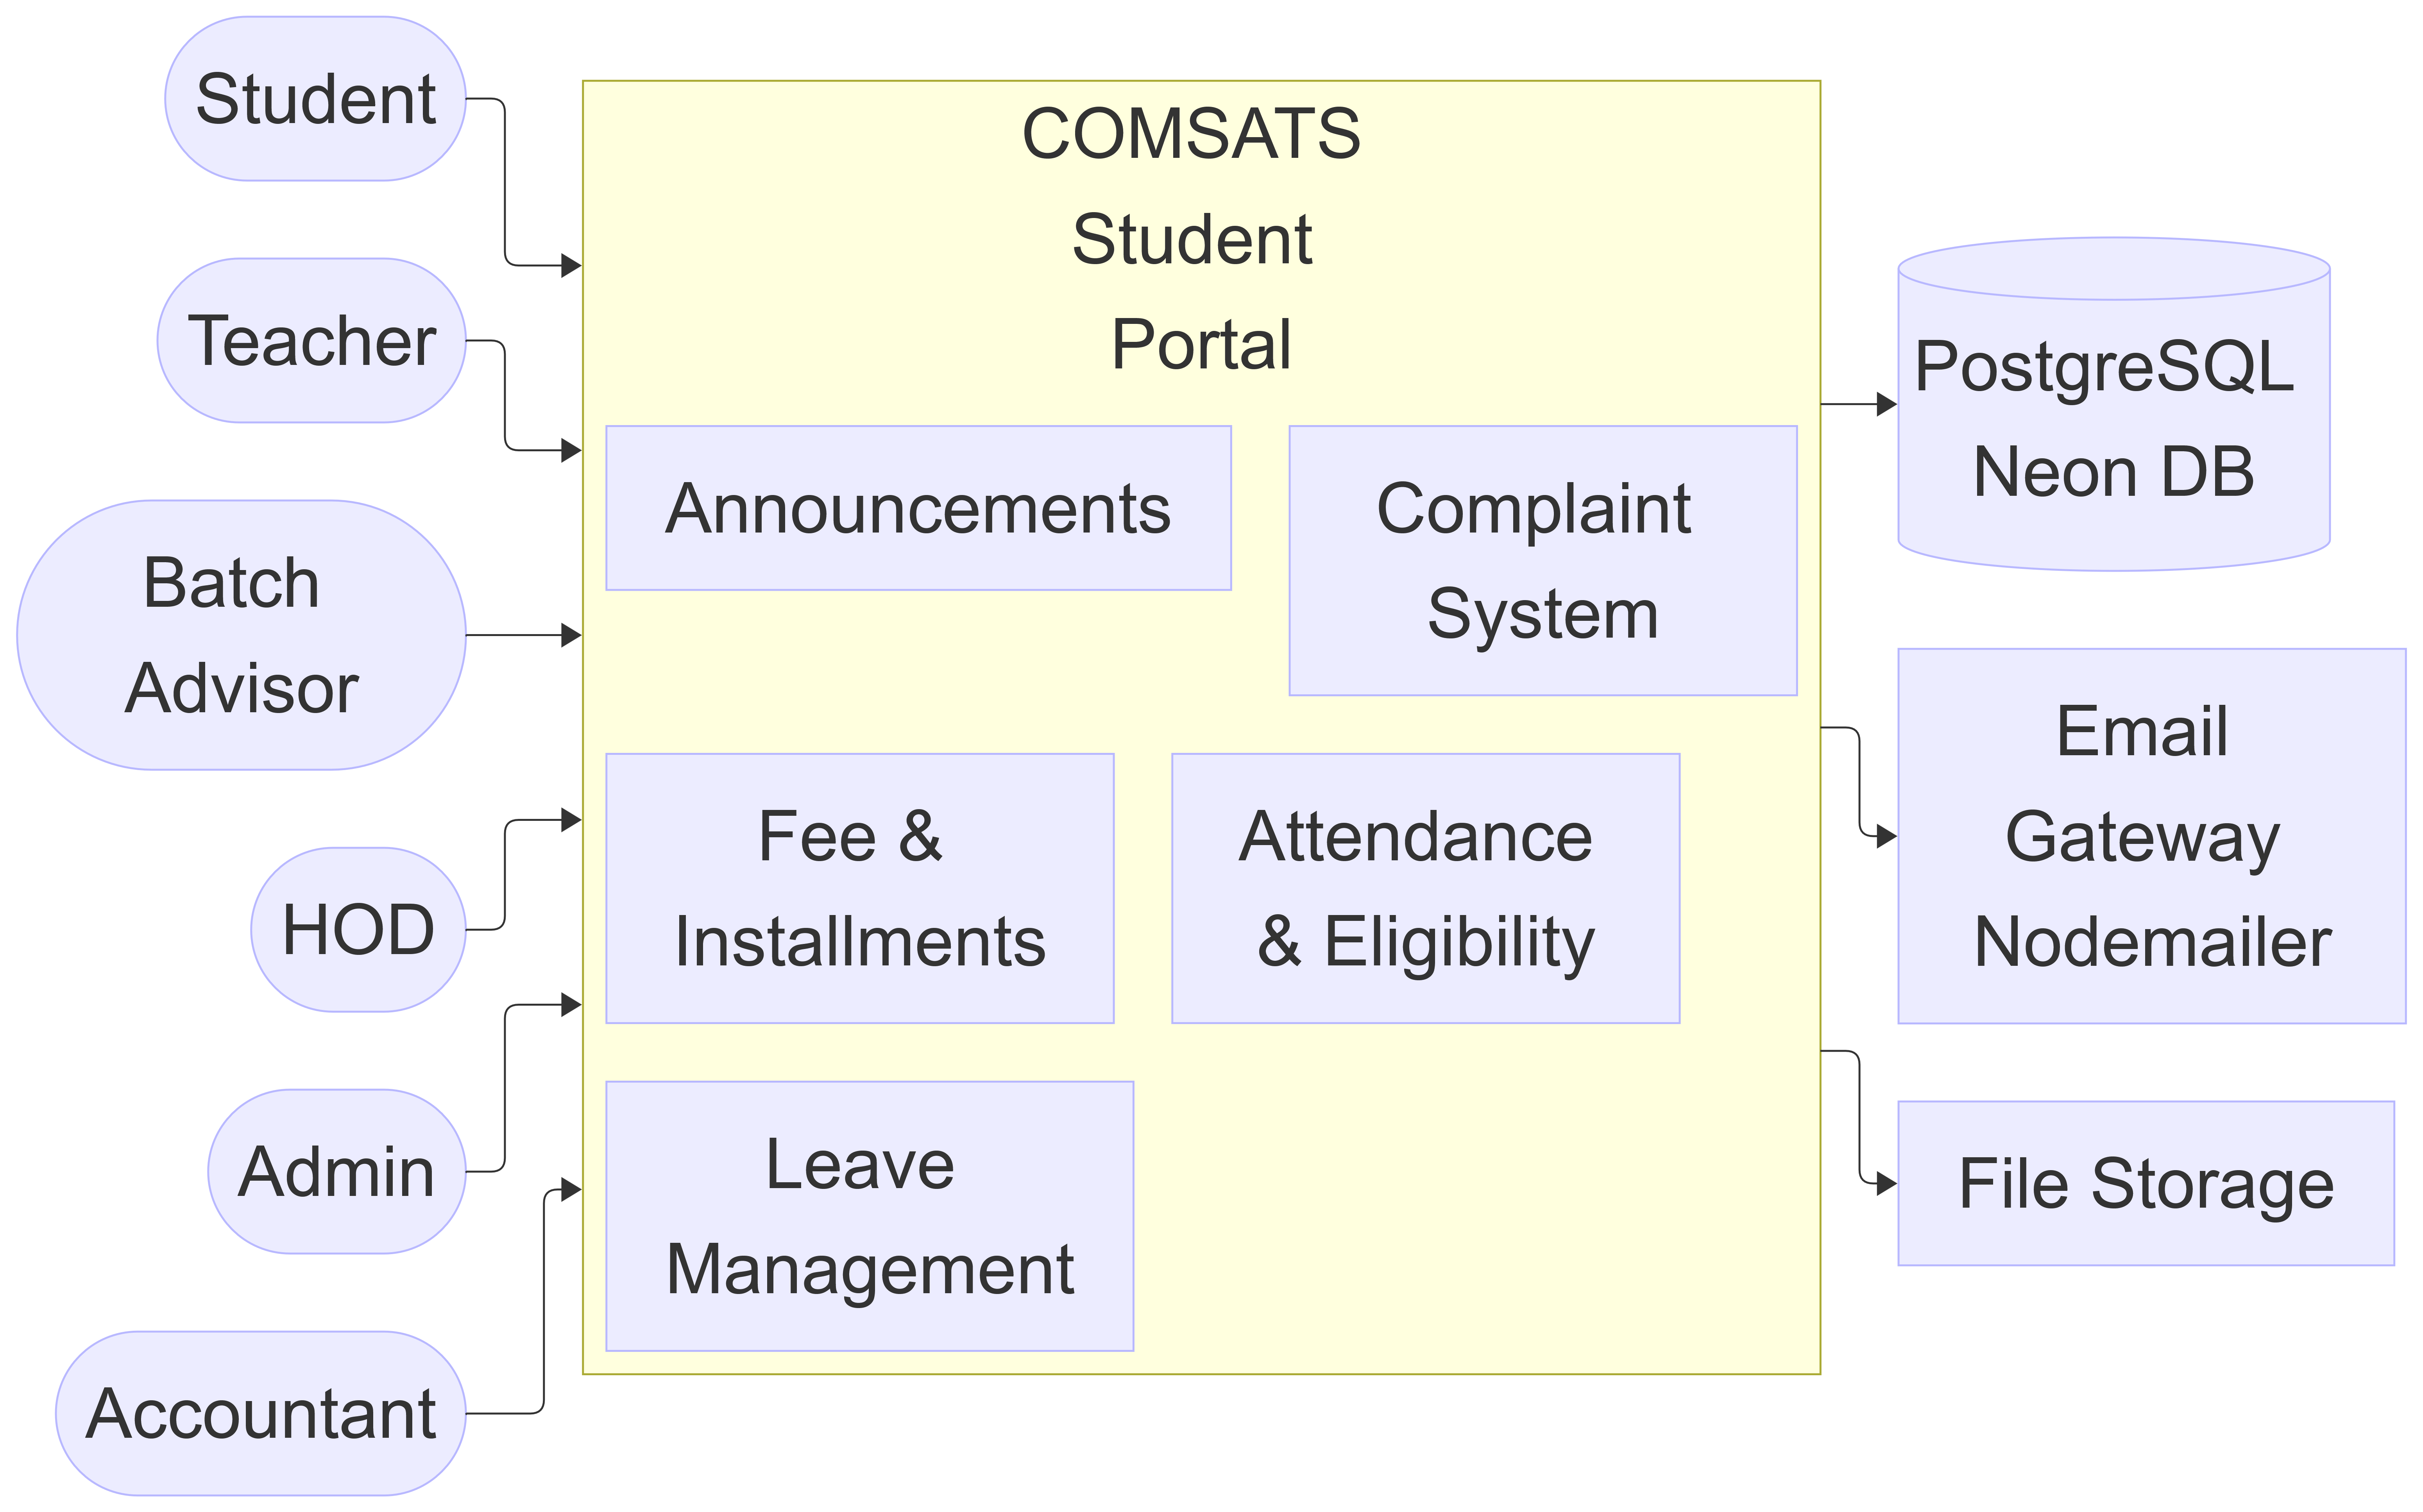
\includegraphics[width=\linewidth]{Figures/diagrams/system-overview.png}
  \caption{System overview}
  \label{fig:system-overview}
\end{figure}


%%%%%%%%%%%%%%%%%%%%%%%%%%%%%%%%%%%%%%%%%%%%%%%%%%%%%%
\section{Architectural Design}

This section describes the high-level architecture of the system.

\begin{figure}[H]
  \centering
  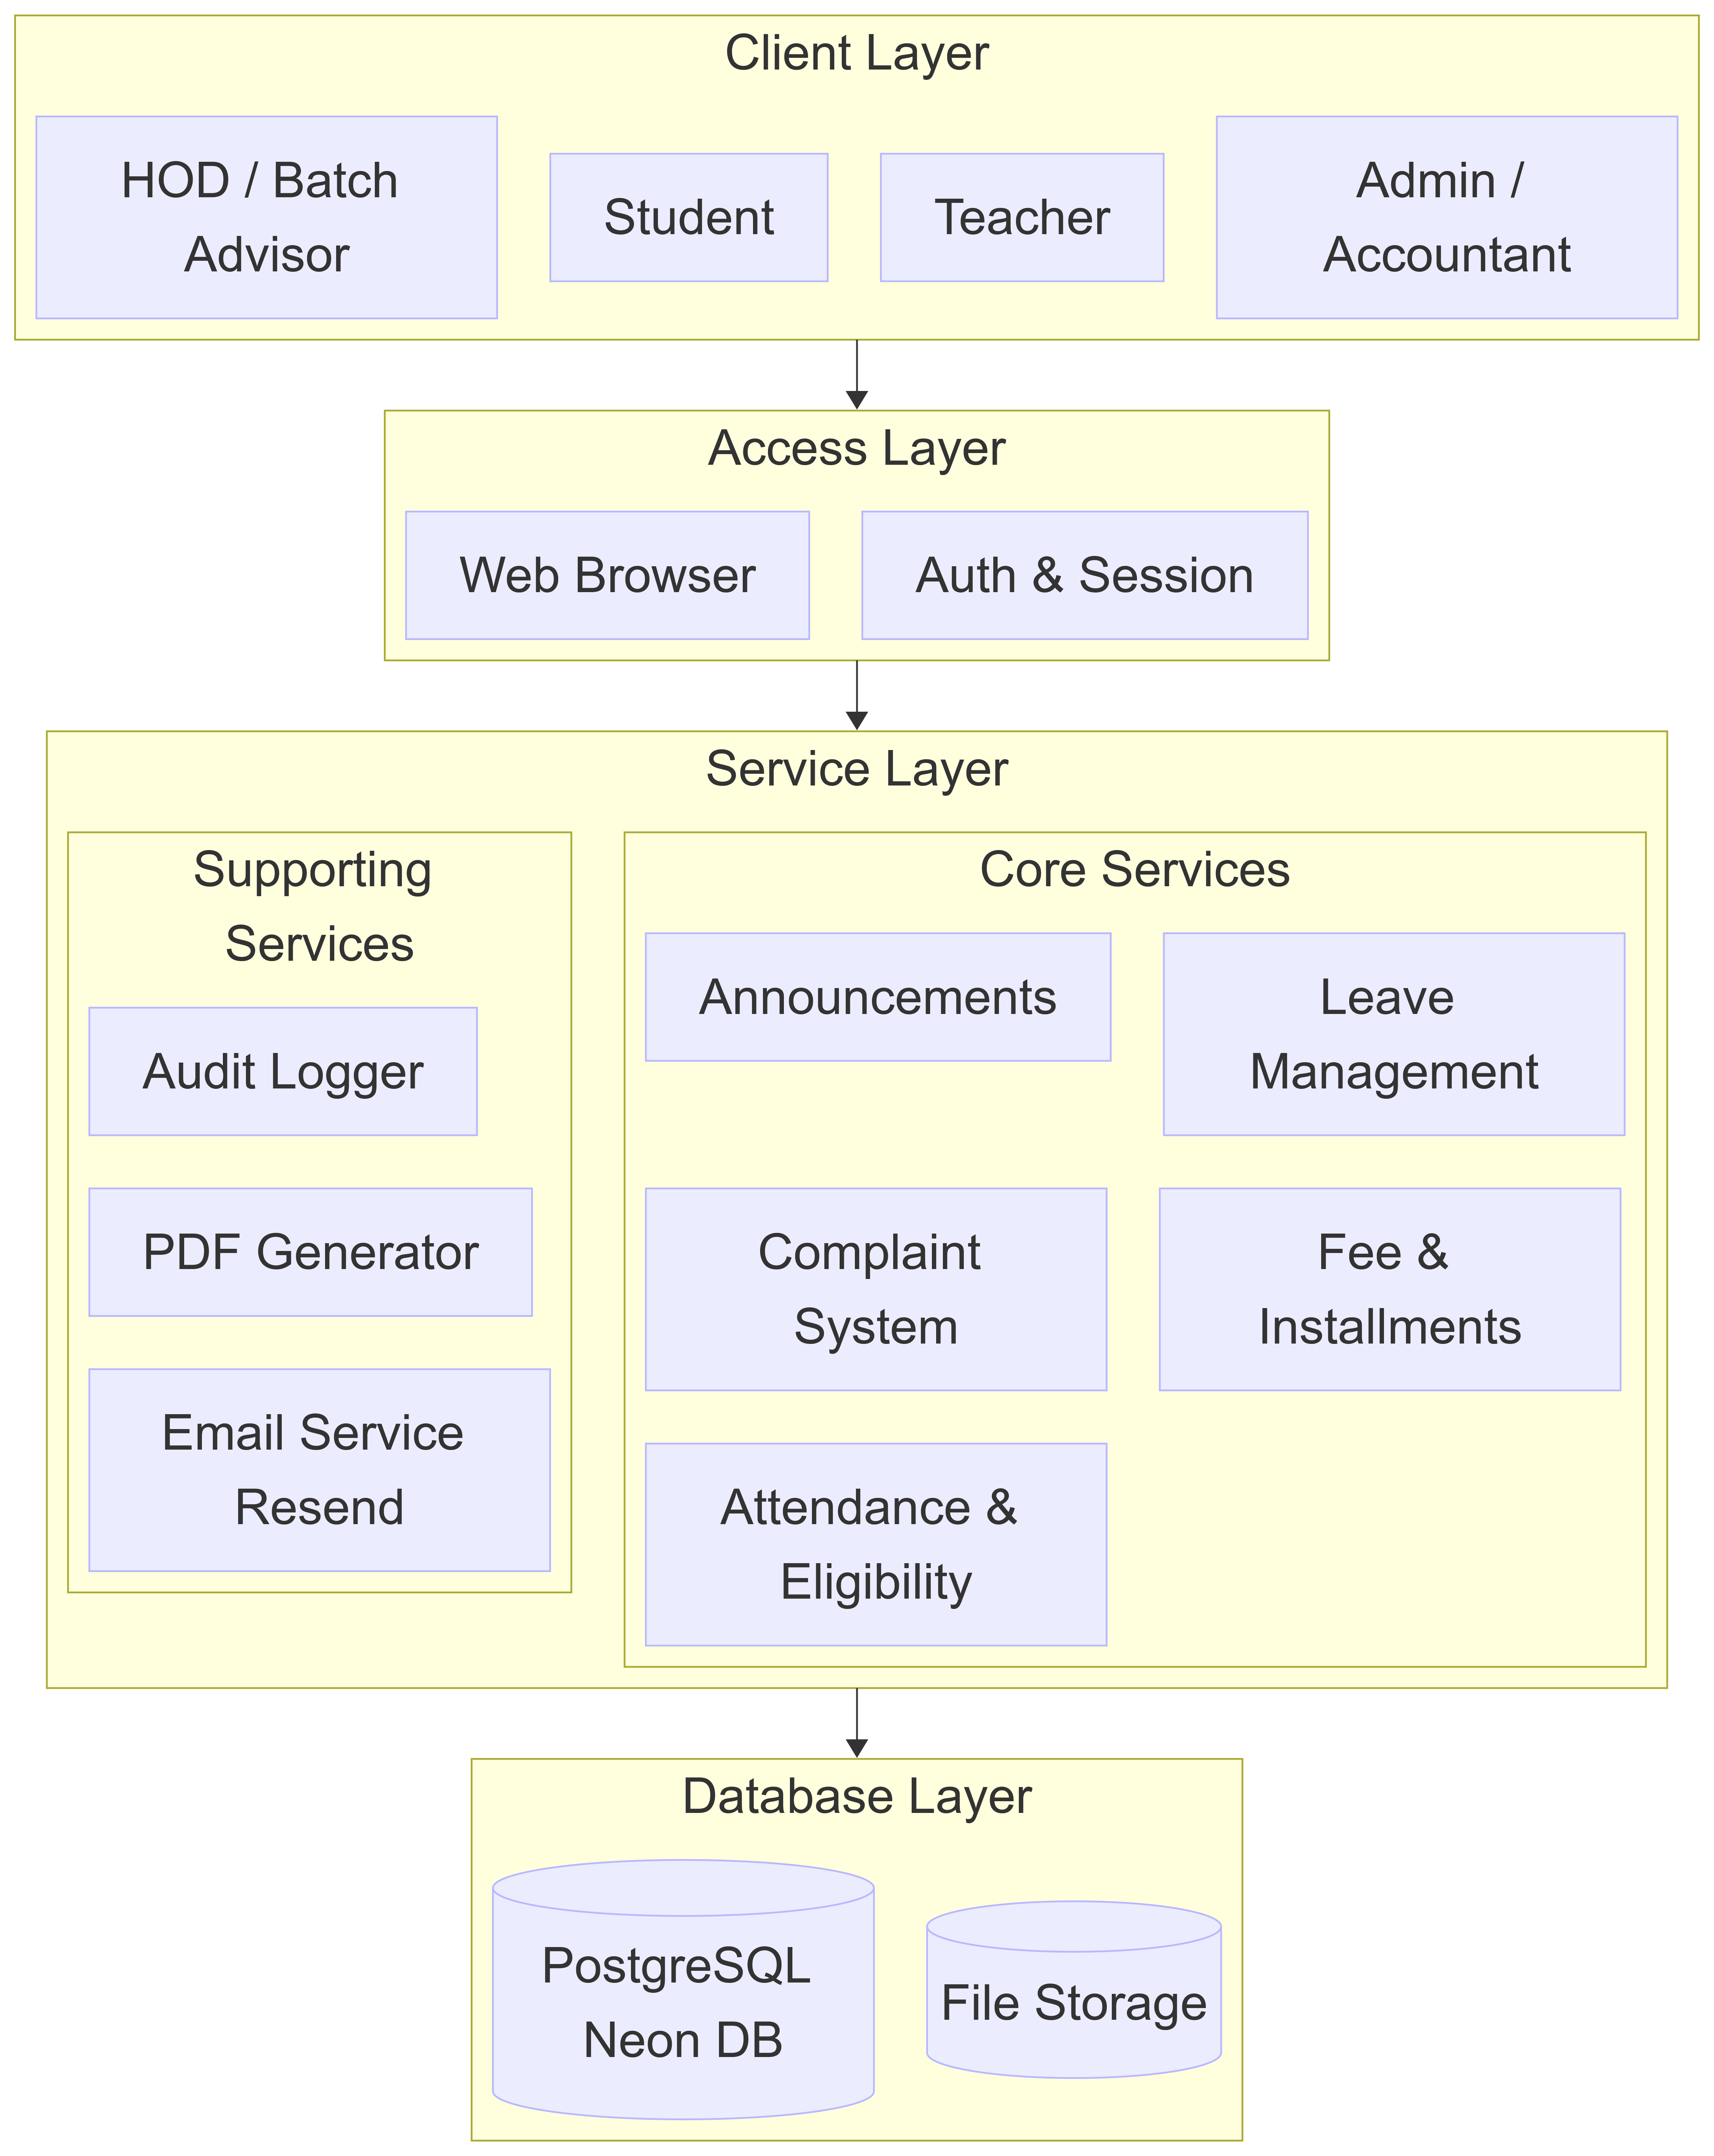
\includegraphics[width=\linewidth]{Figures/diagrams/arch-diagram.png}
  \caption{System overview}
  \label{fig:arch-diagram}
\end{figure}


%%%%%%%%%%%%%%%%%%%%%%%%%%%%%%%%%%%%%%%%%%%%%%%%%%%%%%
\section{Design Models}

This section presents detailed design models of the system. These models describe system behavior, structure, and interactions using UML diagrams. The models help developers understand system workflow before implementation.

%%%%%%%%%%%%%%%%%%%%%%%%%%%%%%%%%%%%%%%%%%%%%%%%%%%%%%
\subsection{Activity Diagrams}

Activity diagrams represent the workflow of different modules of the system.

%%%%%%%%%%%%%%%%%%%%%%%%%%%%%%%%%%%%%%%%%%%%%%%%%%%%%%
\subsubsection{Module 1: Student Leave Request:}

\textbf{Description:}
This diagram how students submit leave request along with validations and approval flow.

\textbf{Start State:} Student is authenticated and navigates to the "Request Leave" page.

\begin{itemize}

    \item \textbf{User Interaction:} Student selects a specific Subject Offering and a Date for the leave request and submits the form.
    \item \textbf{Validation Check:} System performs a concurrency check to ensure no duplicate request exists for the same studentId, subjectOfferingId, and date.
    \item \textbf{Database Interaction:} System creates a new record in the Leave Request table with status as PENDING.
    \item \textbf{Model Interaction:} BA can login and view pending LR and accept or reject LR.
    \begin{itemize}
        \item If accepted status updates to HOD\_PENDING.
        \item If rejected, LR is discarded. End status to rejected.
    \end{itemize}

    \item \textbf{User Interaction Review Phase 2:} HOD logs in and views the HOD\_PENDING LRs. 
    \begin{itemize}
        \item \textbf{Reject:} Update DB status to REJECTED. (End State: Rejected)
        \item \textbf{Accept:} Update DB status to APPROVED. (End State: Approved)
    \end{itemize}

\end{itemize}

\begin{figure}[H]
  \centering
  \includegraphics[width=\linewidth]{Figures/diagrams/act-lr.png}
  \caption{Student Leave Request}
  \label{fig:act-lr}
\end{figure}

%%%%%%%%%%%%%%%%%%%%%%%%%%%%%%%%%%%%%%%%%%%%%%%%%%%%%%

\subsubsection{Module 2: Student Create Complaint:}

\textbf{Description:}
This diagram how students submit complaints along with validations and approval flow.

\begin{itemize}
    \item \textbf{Start State:} Student is authenticated and opens the "File Complaint" form.
    \item \textbf{Creation \& Validation:} Student submits title, details, and category. After validating required fields, the system creates a Complaint record in the database with status BA\_PENDING, defaulting to the student's department.
    \item \textbf{BA Decision:} The BA reviews the queue and decides to either Reject or Accept.
    \item \textbf{HOD Final Action:} The HOD reviews HOD\_PENDING complaints. Decisions include:
    HOD\_ACCEPTED, HOD\_REJECTED, or ASSIGNED (to another department).
    
    \item \textbf{End State:} Status is finalized as HOD\_ACCEPTED, HOD\_REJECTED, ASSIGNED, or BA\_REJECTED.
\end{itemize}


\begin{figure}[H]
  \centering
  \includegraphics[width=\linewidth]{Figures/diagrams/act-compl.png}
  \caption{Student Create Complaint}
  \label{fig:act-compl}
\end{figure}


%%%%%%%%%%%%%%%%%%%%%%%%%%%%%%%%%%%%%%%%%%%%%%%%%%%%%%
\subsubsection{Module 3: HOD/ACC announcemnt}

\textbf{Description:}
HOD creates for their department students. Accountant can select specific departments to create announcements. Ann can be published and scheduled for specific date.

Start State: Author (HOD or Accountant) is authenticated and opens the ``Create Announcement'' form.

\begin{itemize}
    \item \textbf{User Interaction}: Author enters title, content, announcement type, and sets optional audience filters (Department, Program, Batch, Year).

    \item \textbf{Validation Check}: System validates that required fields are present and that any scheduledFor date is in the future (within a 2-day limit).

    \item \textbf{Decision (Publish Mode)}: Author selects one of three modes:
    \begin{itemize}
        \item \textit{Immediate}: Proceed to step 4.
        \item \textit{Draft}: Skip to Step 5 (Status: DRAFT).
        \item \textit{Scheduled}: Proceed to step 4 with a target date time.
    \end{itemize}

    \item \textbf{Database/Model Interaction}: System creates/updates the Ann:
    \begin{itemize}
        \item \textit{Immediate}: Status PUBLISHED.
        \item \textit{Scheduled}: Status SCHEDULED, target date.
        \item \textbf{Background Interaction}: For SCHEDULED, system queues an Inngest job to wake up at the target date time.
    \end{itemize}

    \item \textbf{Decision (Inngest Execution)}:
    \begin{itemize}
        \item When scheduled For is reached, Inngest wakes up and updates DB status to PUBLISHED and sets published At.
    \end{itemize}

    \item \textbf{End State (Visibility)}:
    \begin{itemize}
        \item \textit{Draft}: Announcement saved in DB; End State: Hidden/Draft.
        \item \textit{Published}: Announcement is visible to students matching the audience filters; End State: Live.
    \end{itemize}
\end{itemize}

\begin{figure}[H]
  \centering
  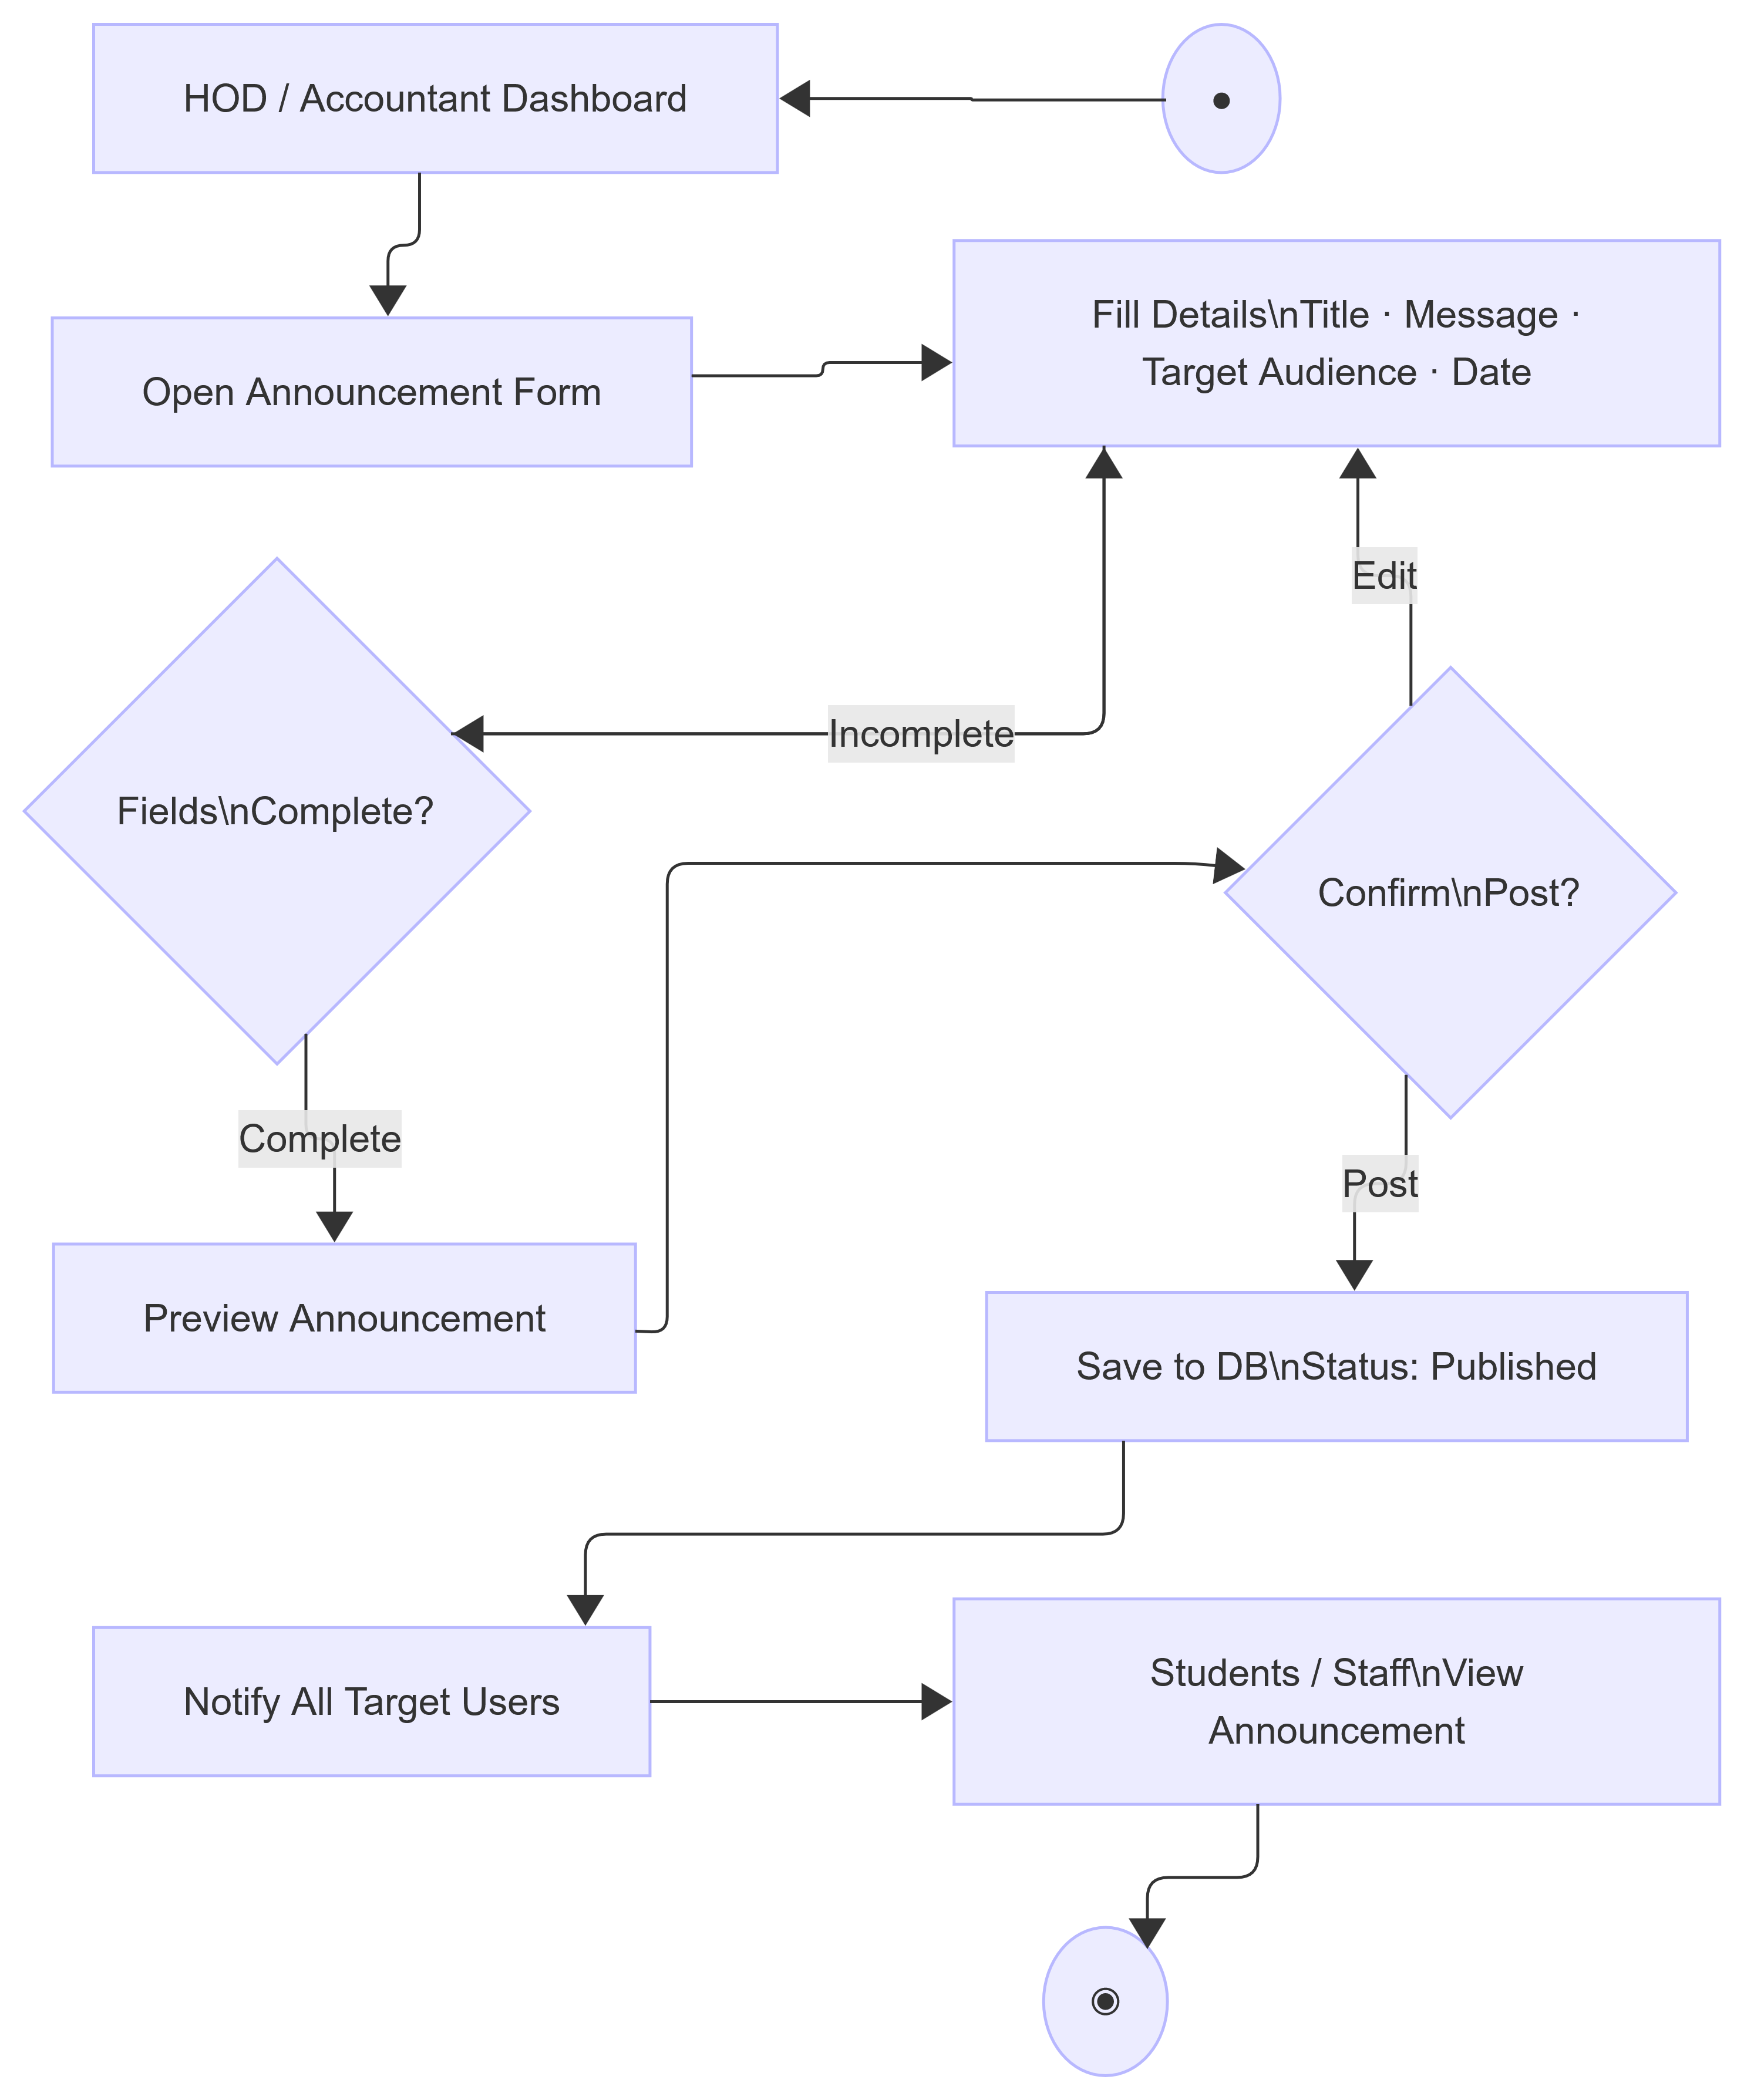
\includegraphics[width=\linewidth]{Figures/diagrams/act-ann.png}
  \caption{Announcement}
  \label{fig:act-ann}
\end{figure}

%%%%%%%%%%%%%%%%%%%%%%%%%%%%%%%%%%%%%%%%%%%%%%%%%%%%%%

\textbf{Figure 4: Fee Installments}

\subsubsection{Module 4: Fee Installment Request}
\textbf{Description:}
Students can request to split their due fee into installments. The accountant pre-defines the base installment structure (e.g., 70+30 of 100). A student may further split any due installment, subject to a maximum of 3 total installments. Each request goes through a two-level approval chain: HOD reviews first, then the Accountant confirms.

\textbf{Start State:} Student is authenticated, views the current fee structure and outstanding balance, and opens the ``Request Installment'' form.

\begin{itemize}
    \item \textbf{User Interaction}: Student enters the amount they wish to pay now against an outstanding installment (e.g., pay 50 of a 70 due amount).
    \item \textbf{Validation Check}: System validates two conditions:
    \begin{itemize}
        \item \textit{Amount Valid}: Requested amount must be greater than zero and less than or equal to the outstanding installment amount.
        \item \textit{Count Check}: Total number of installment requests for this fee cycle must be fewer than 3. If the limit is reached, the request is blocked and the student is notified.
    \end{itemize}
    \item \textbf{Database/Model Interaction}: On passing both checks, a new installment request record is saved with status \texttt{PENDING}, and the remaining balance is split accordingly (e.g., 50 paid now, remaining 20+30 deferred).
    \item \textbf{Decision (HOD Review)}: HOD is notified and reviews the request.
    \begin{itemize}
        \item \textit{Reject}: Request is marked \texttt{REJECTED}; student is notified. End State: Rejected.
        \item \textit{Approve}: Request is forwarded to the Accountant.
    \end{itemize}
    \item \textbf{Decision (Accountant Review)}: Accountant reviews the HOD-approved request.
    \begin{itemize}
        \item \textit{Reject}: Request is marked \texttt{REJECTED}; student is notified. End State: Rejected.
        \item \textit{Approve}: Request is marked \texttt{APPROVED} and balance records are updated.
    \end{itemize}
    \item \textbf{Post-Approval}: System generates a fee voucher for the approved amount and notifies the student.
    \item \textbf{Decision (Balance Check)}: System checks whether the remaining balance is zero.
    \begin{itemize}
        \item \textit{Balance Remaining}: Student may submit another installment request (loop back to step 1), provided the count limit has not been reached.
        \item \textit{Balance Zero}: No further requests possible. End State: Account fully settled.
    \end{itemize}
\end{itemize}

\begin{figure}[H]
  \centering
  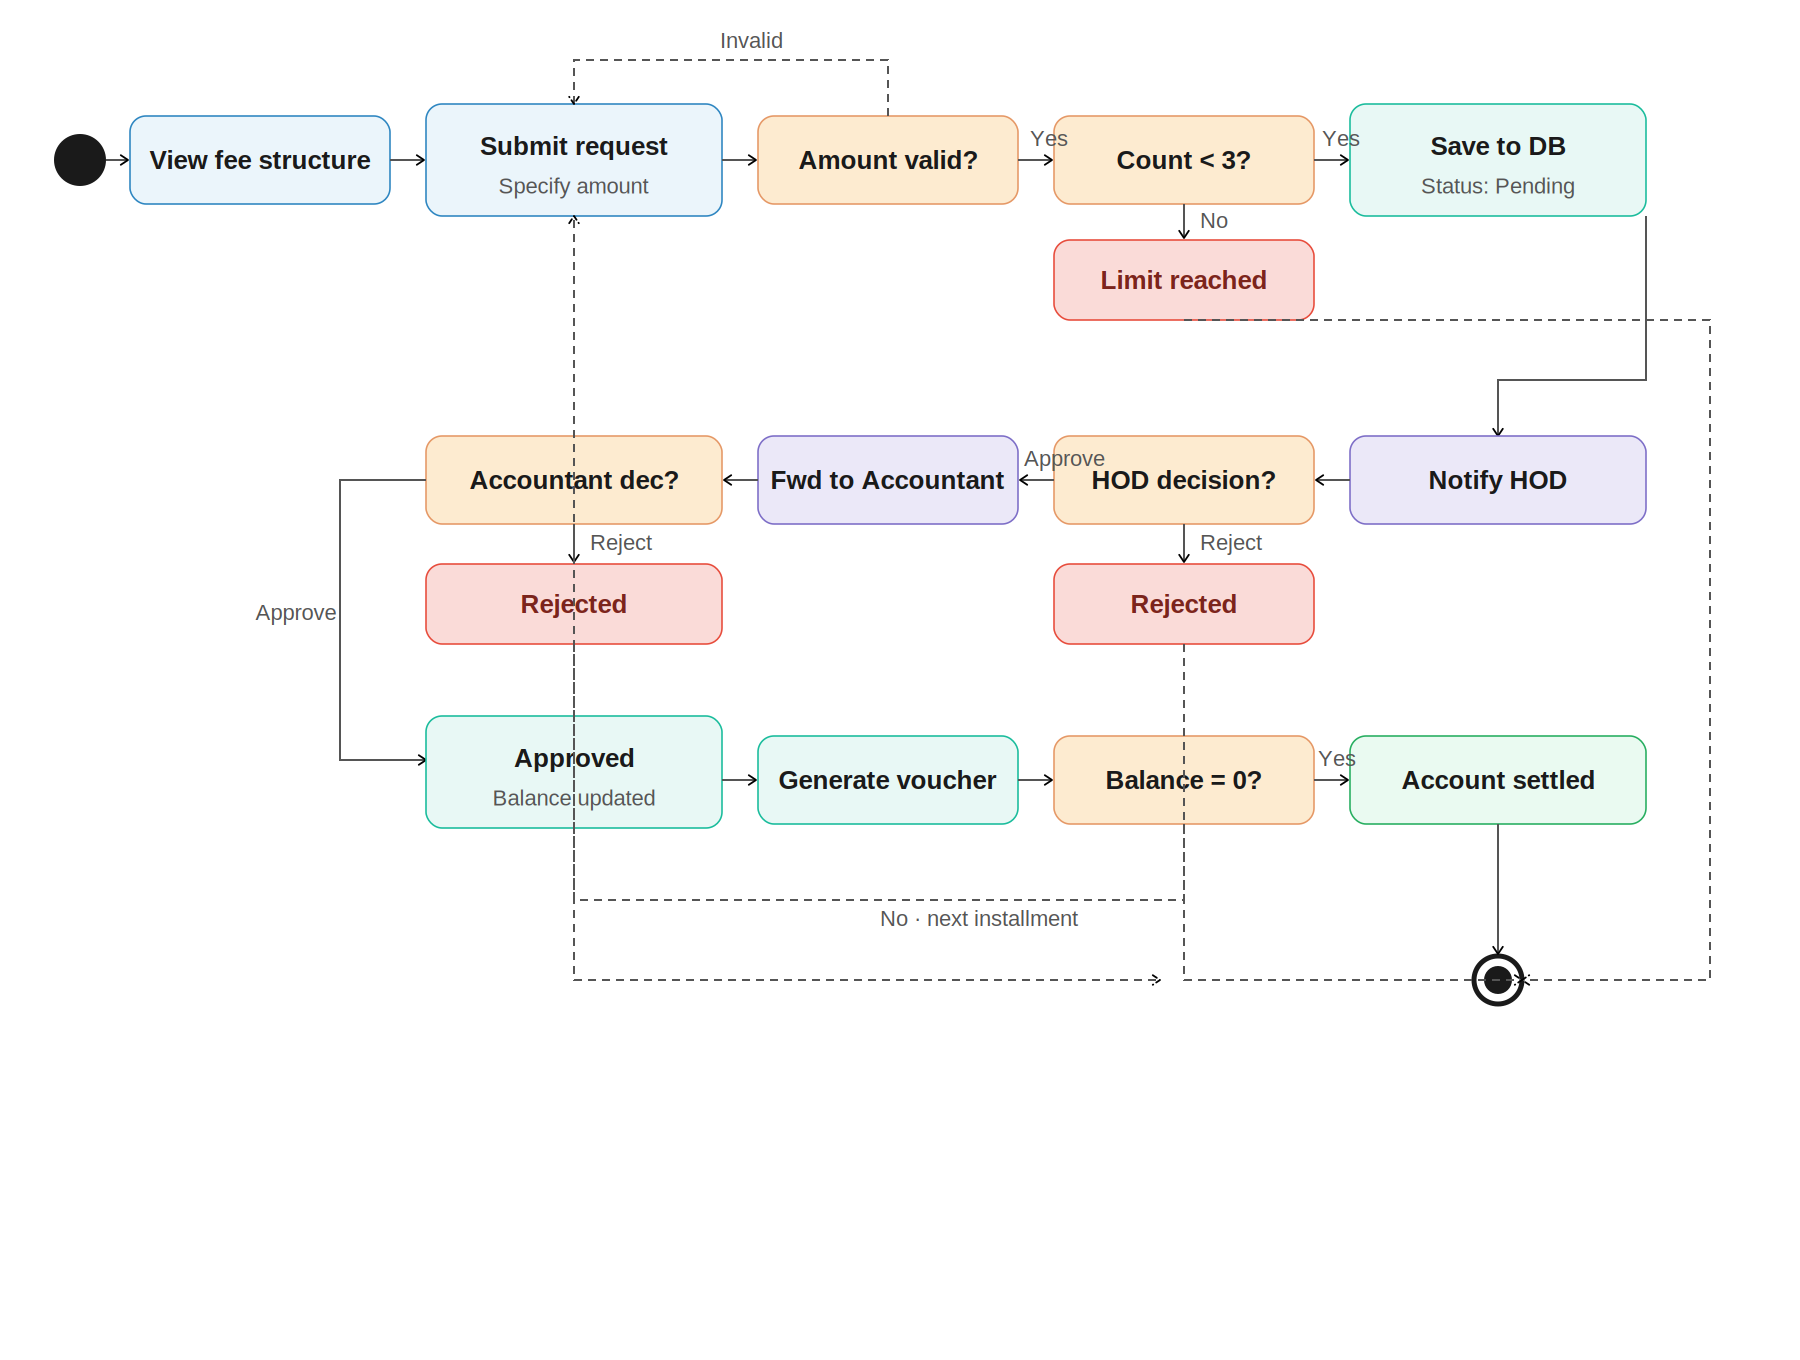
\includegraphics[width=\linewidth]{Figures/diagrams/act-fee.png}
  \caption{Fee Installments}
  \label{fig:act-fee}
\end{figure}

%%%%%%%%%%%%%%%%%%%%%%%%%%%%%%%%%%%%%%%%%%%%%%%%%%%%%%
\subsection{Class Diagram}

The class diagram shows the static structure of the system.

\subsubsection{User Roles and Permissions Overview}

The system implements a Role-Based Access Control (RBAC) model with a central User entity extended by role-specific profiles.

Inheritance and composition:
\begin{itemize}
    \item Every specialized role (Student, Professor, BA, HOD, Accountant) is linked to exactly one \texttt{User} (1-to-0..1 relationship).
    \item A Professor can be promoted to BA (additional 1-to-0..1 link).
\end{itemize}

This structure enables fine-grained access control while maintaining a single authentication entry point and allowing role escalation within the same department.

\begin{figure}[H]
  \centering
  \includegraphics[width=\linewidth]{Figures/diagrams/class/class-user-role.png}
  \caption{Class diagram - user roles}
  \label{fig:class-user-role}
\end{figure}

%%%%%%%%%%%%%%%%%%%%%%%%%%%%%%%%%%%%%%%%%%%%%%%%%%%%%%
\subsubsection{Leave Request and Attendance Synchronization}

The leave management module enables students to request absences with automatic impact on attendance records.

A \texttt{Student} submits a \texttt{LeaveRequest} for a specific date, providing a reason title, details, and linking it to the relevant \texttt{SubjectOffering} (course instance defined by semester, year, and department).

The request follows departmental approval workflow:
- First reviewed and forwarded by the \texttt{BA} of the student's department.
- Then finally approved or rejected by the \texttt{HOD}.

\begin{figure}[H]
  \centering
  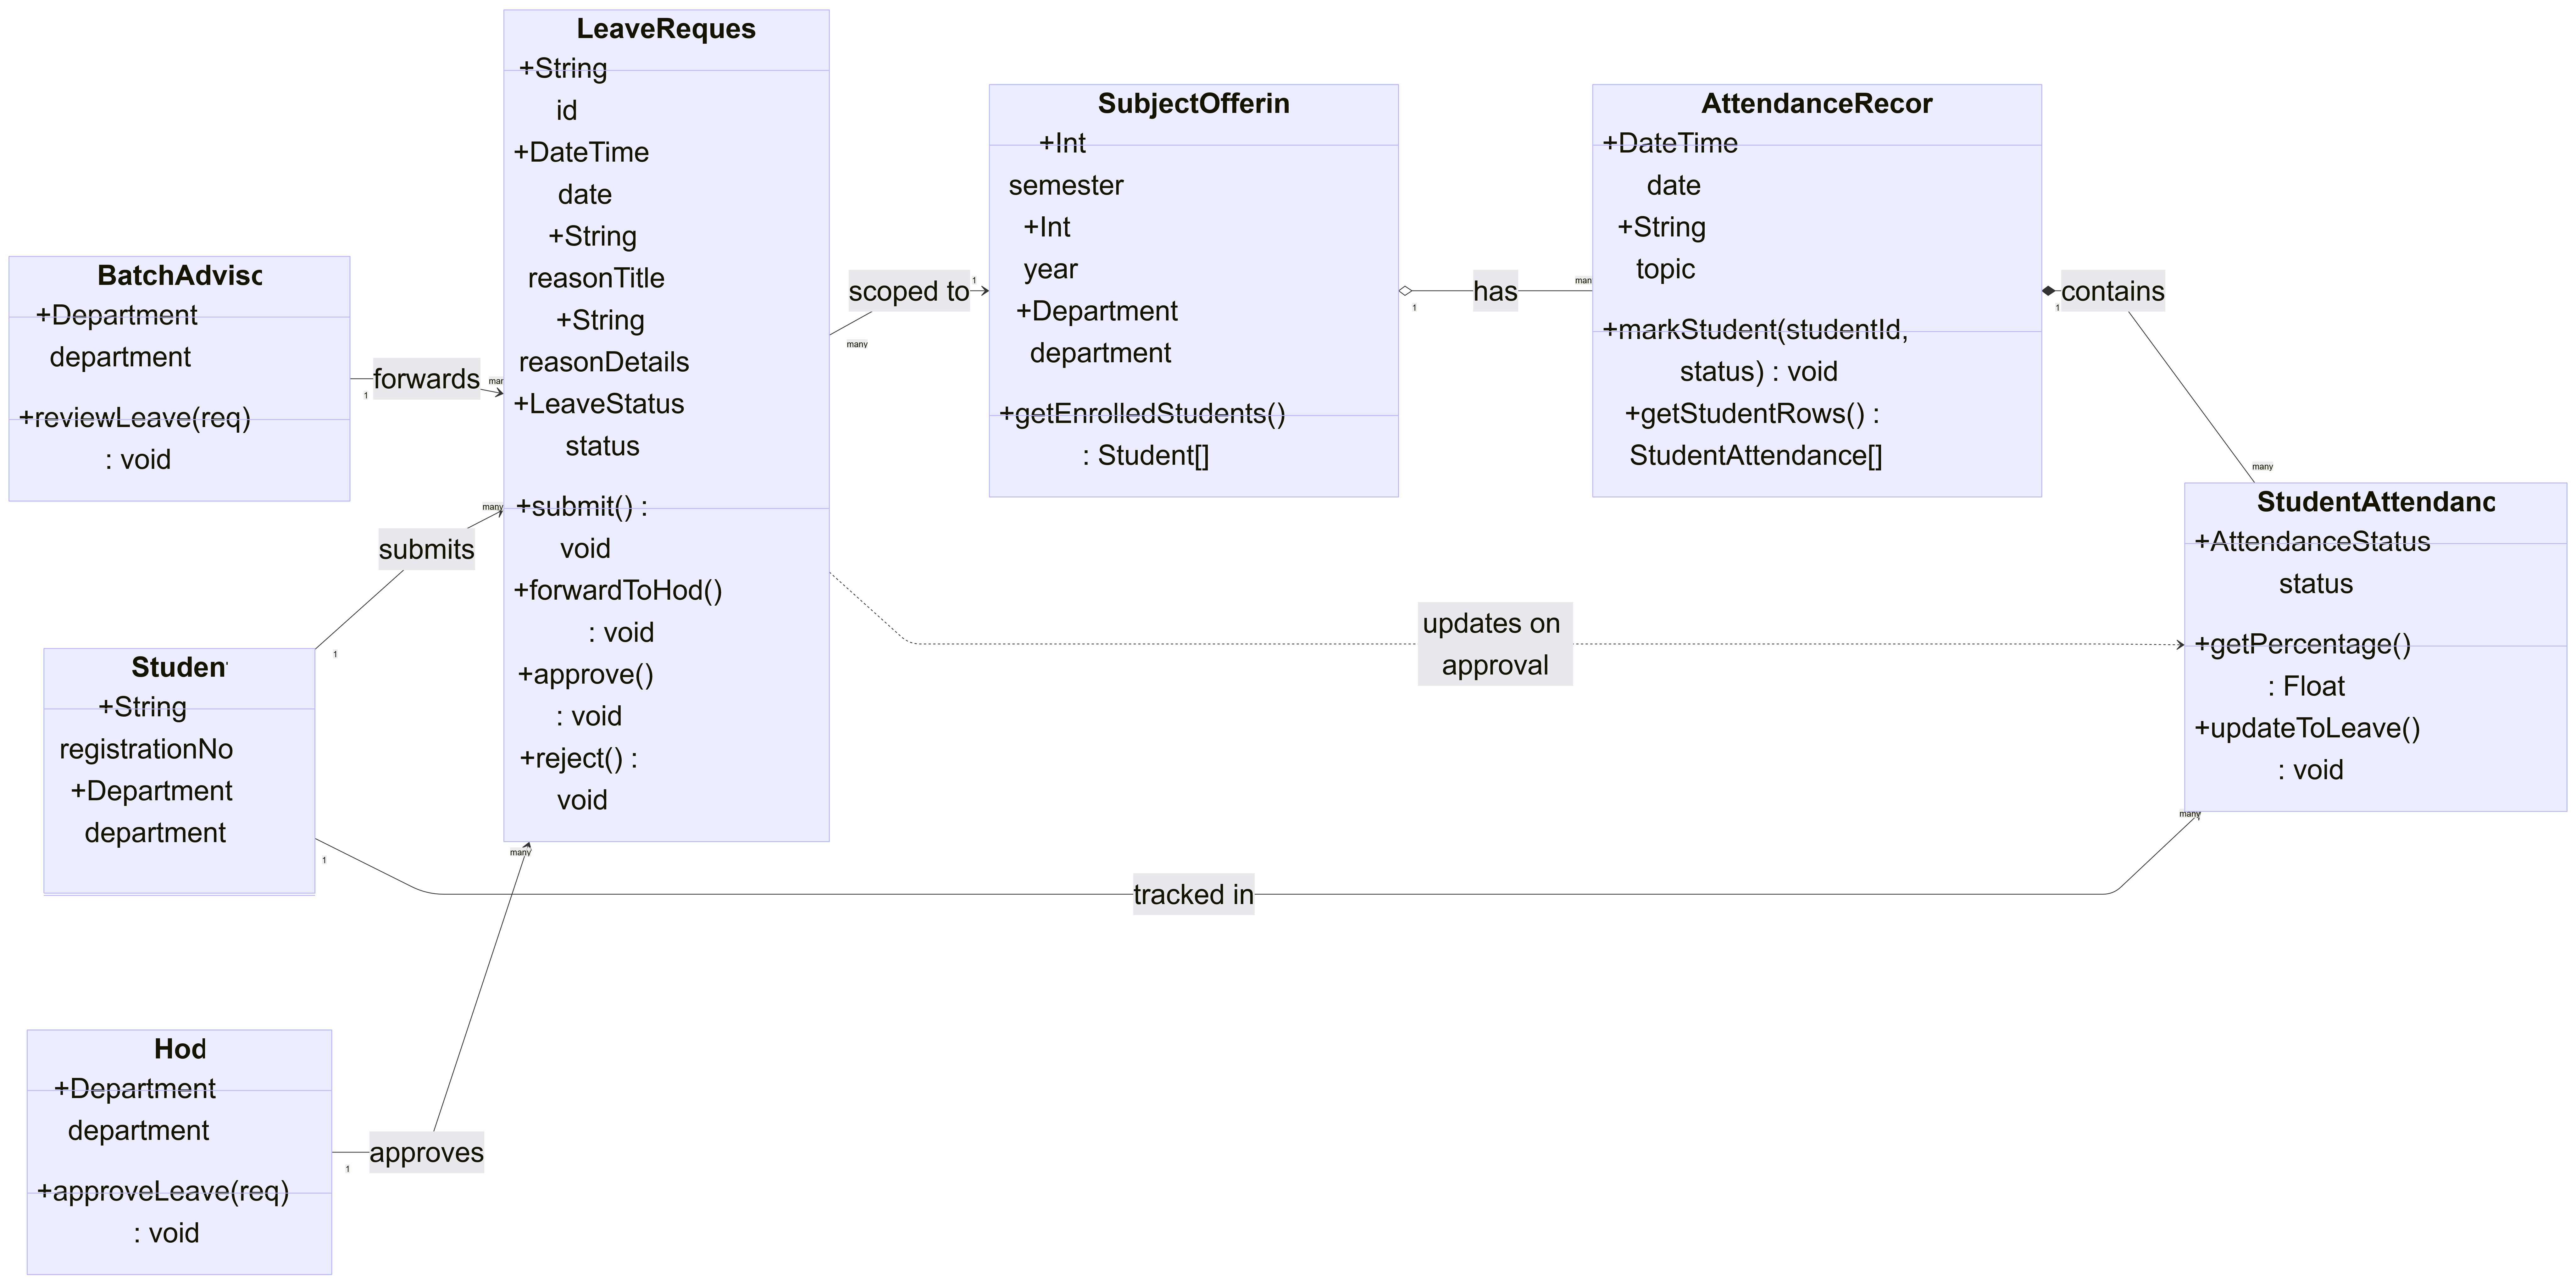
\includegraphics[width=\linewidth]{Figures/diagrams/class/class-lr.png}
  \caption{Class diagram - Leave requests}
  \label{fig:class-lr}
\end{figure}

%%%%%%%%%%%%%%%%%%%%%%%%%%%%%%%%%%%%%%%%%%%%%%%%%%%%%%
\subsubsection{Complaint Submission and Resolution Process}

The complaint system provides a structured mechanism for students to report issues, with departmental review, reassignment capability, and complete action auditing.

A \texttt{Student} submits a \texttt{Complaint} specifying the category, title, target department, and description. The complaint enters a lifecycle with status tracking.

Tracking and transparency features:
\begin{itemize}
    \item Every review, status transition, or remark is logged in \texttt{ComplaintReview} entries.
\end{itemize}

Key entities:
\begin{itemize}
    \item \textbf{Student} files complaints tied to their registration number and department.
    \item \textbf{Complaint} holds core data (category, title, status, target department, BA/HOD remarks) and controls the submission–review–resolution workflow.
    \item \textbf{ComplaintReview} maintains an immutable history of all actions performed on a complaint.
    \item \textbf{BatchAdvisor} conducts initial departmental review.
    \item \textbf{Hod} holds final decision authority (resolve, reject, reassign).
\end{itemize}

\begin{figure}[H]
  \centering
  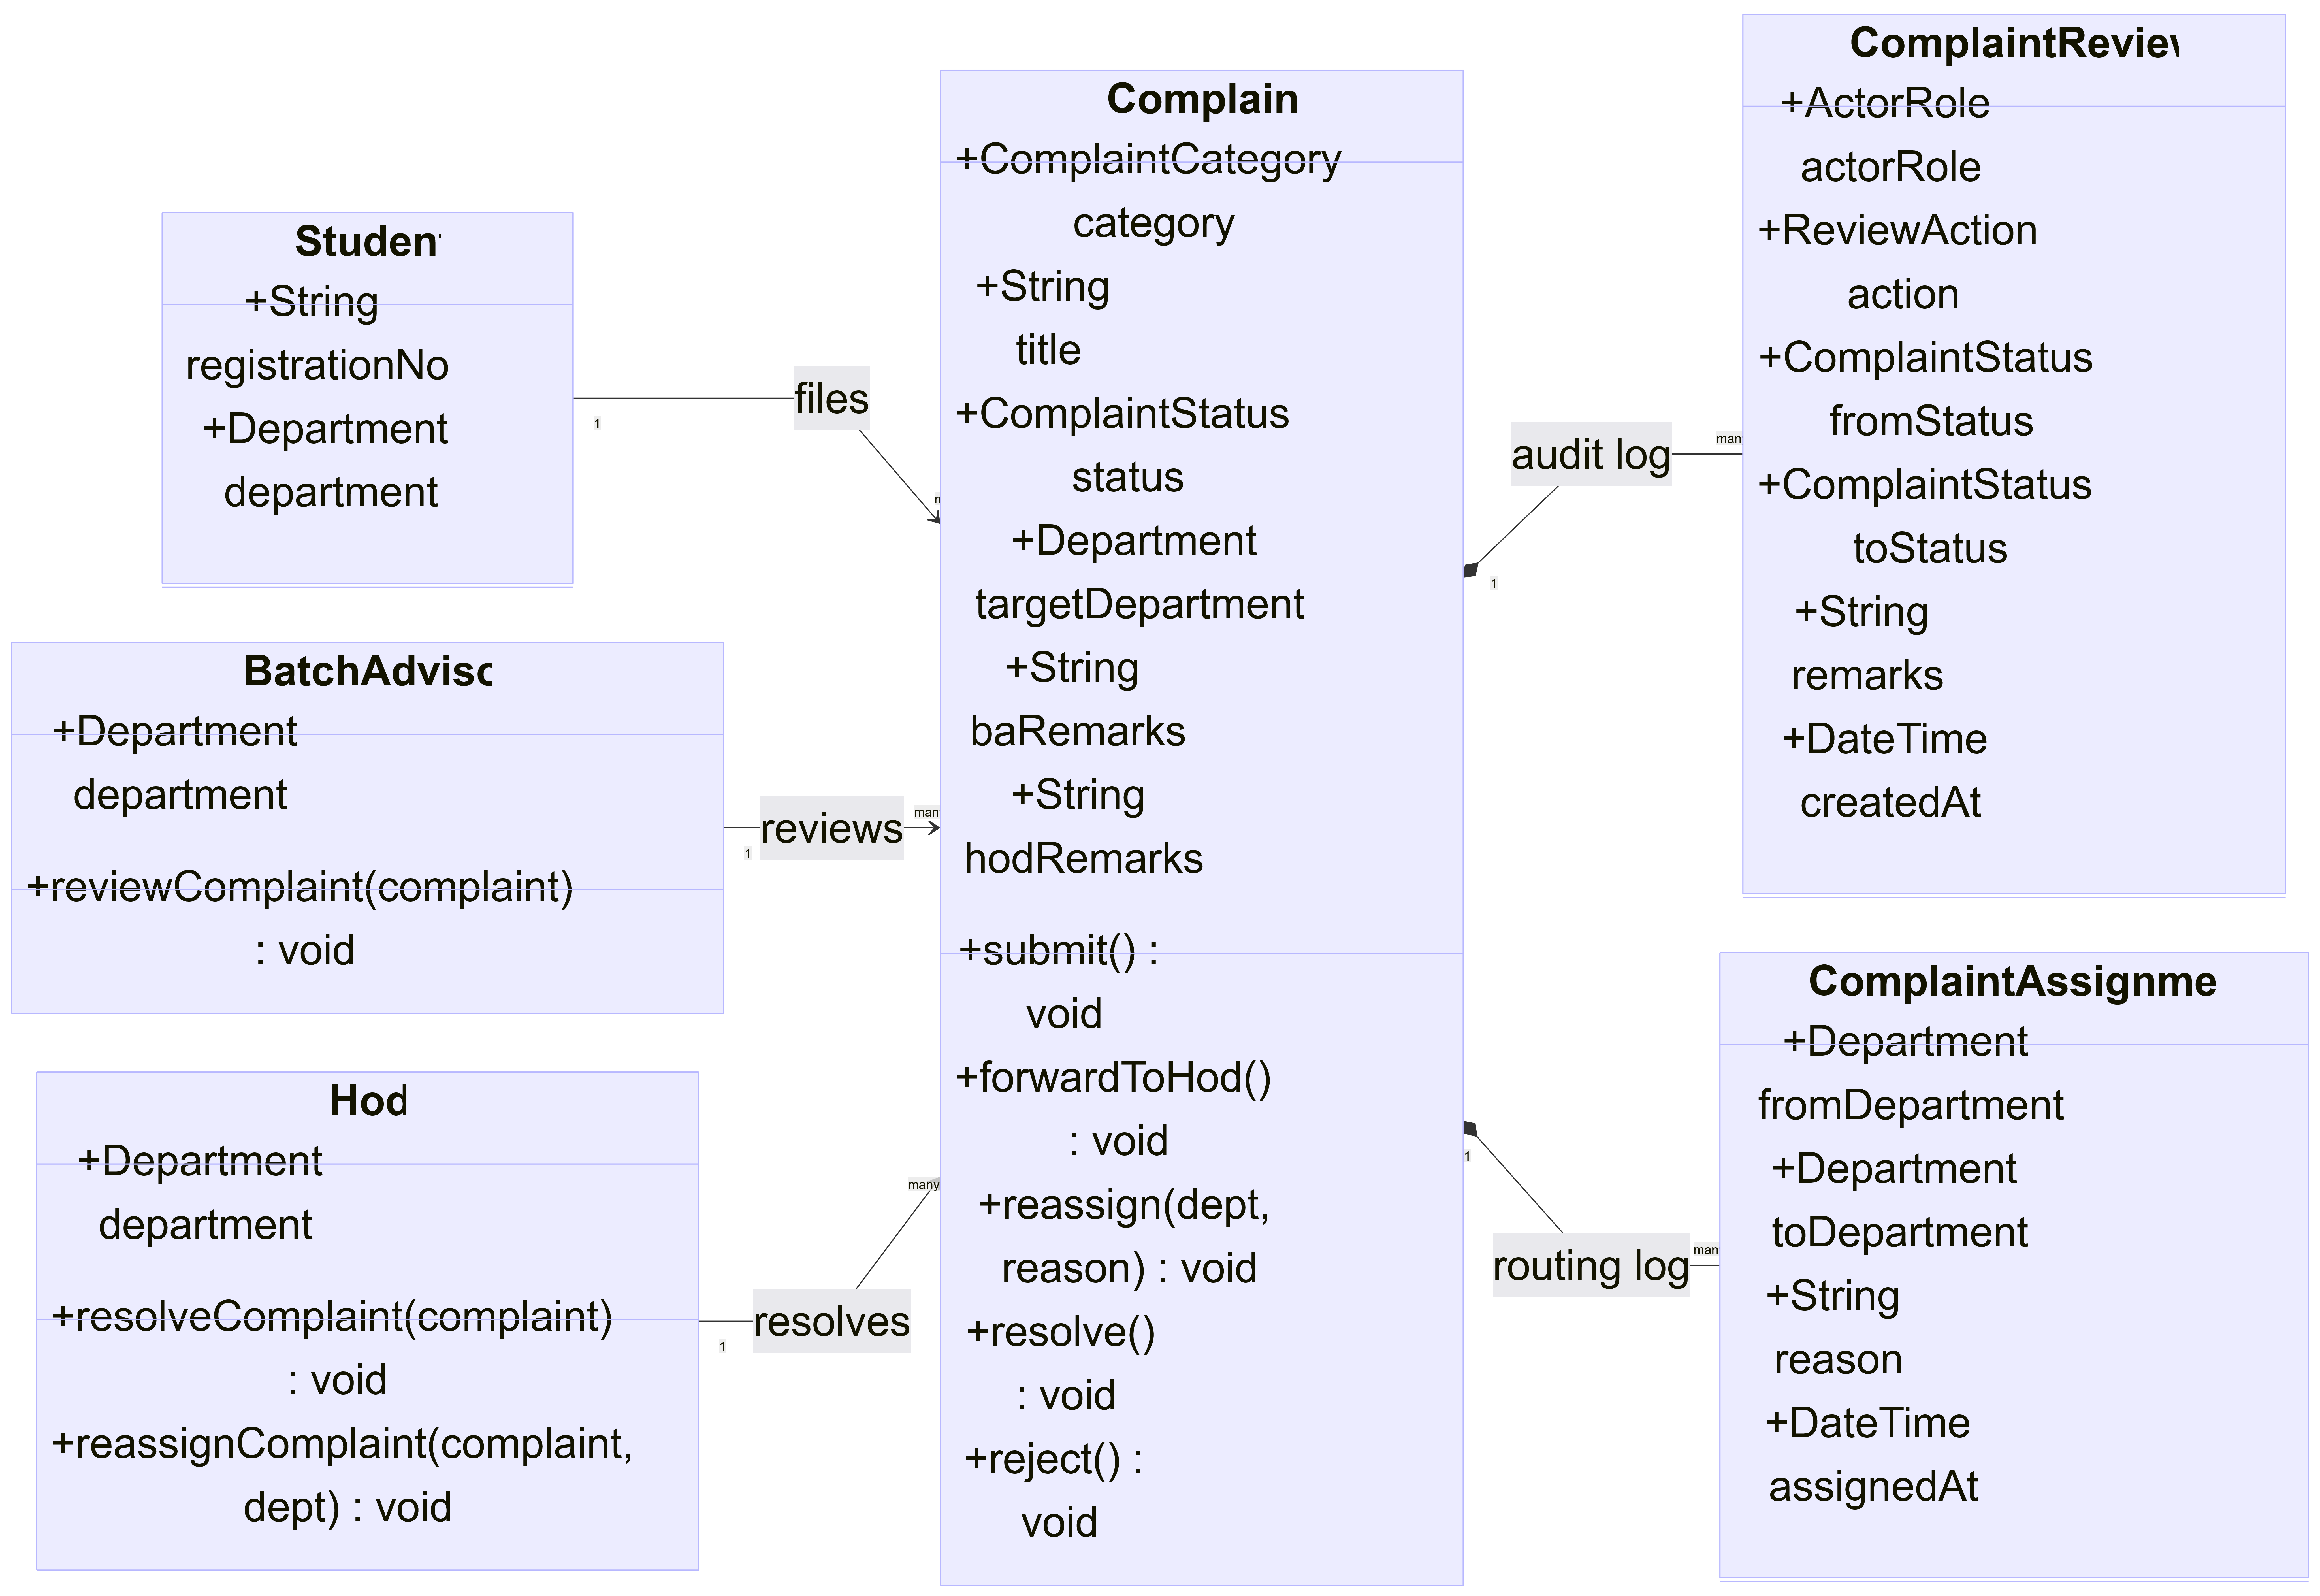
\includegraphics[width=\linewidth]{Figures/diagrams/class/class-compl.png}
  \caption{Class diagram - Complaint}
  \label{fig:class-compl}
\end{figure}

%%%%%%%%%%%%%%%%%%%%%%%%%%%%%%%%%%%%%%%%%%%%%%%%%%%%%%
\subsection{Sequence Diagrams}

Sequence diagrams show interaction between objects over time.

%%%%%%%%%%%%%%%%%%%%%%%%%%%%%%%%%%%%%%%%%%%%%%%%%%%%%%
\subsubsection{Sequence Diagram – User Login}

The authentication process follows a standard credential-based login with session/token management.

\begin{itemize}
    \item User submits email/password via the login form.
    \item Next.js form forwards credentials to the better-auth auth service.
    \item Auth service verifies credentials in the database.
    \item On success:
    \begin{itemize}
        \item A secure session/token is created and stored.
        \item Token is returned to Next.js.
        \item Next.js sets an HttpOnly cookie and redirects to the user dashboard.
    \end{itemize}
    \item On failure:
    \begin{itemize}
        \item 401 Unauthorized response is sent back.
        \item Browser displays error message (invalid credentials).
    \end{itemize}
\end{itemize}

\begin{figure}[H]
  \centering
  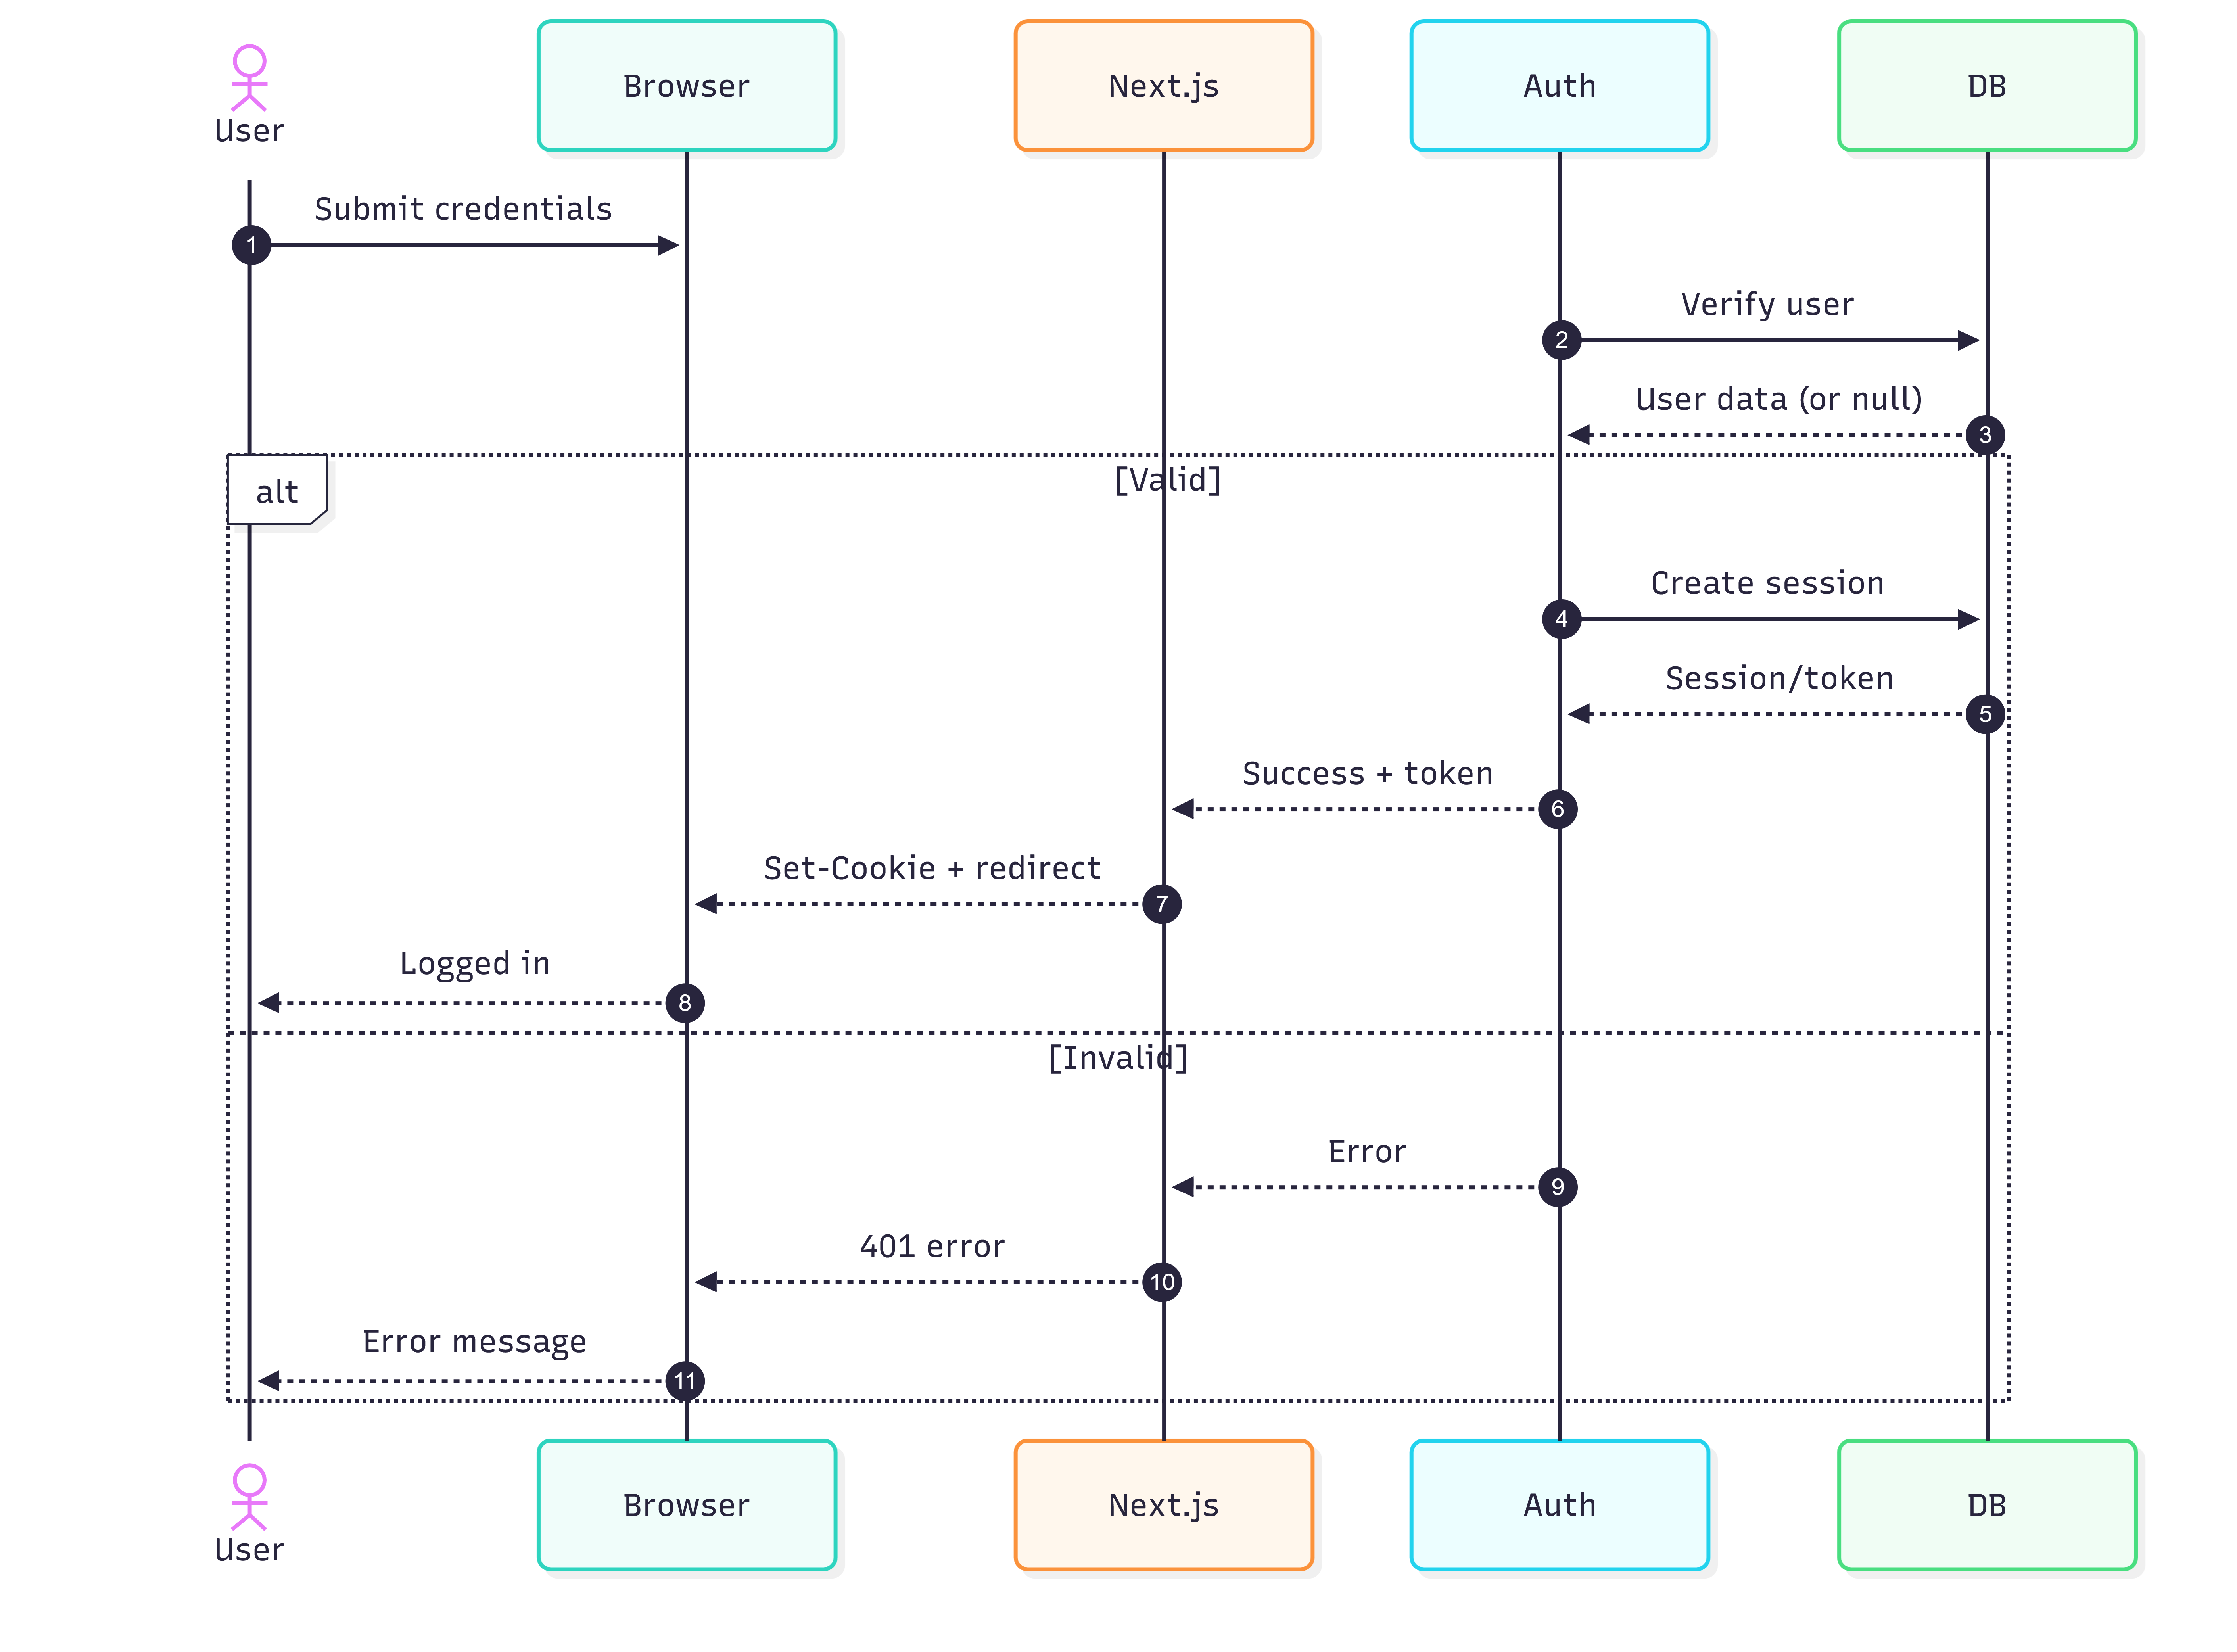
\includegraphics[width=\linewidth]{Figures/diagrams/seq/seq-login.png}
  \caption{Sequence diagram - Login}
  \label{fig:seq-login}
\end{figure}

%%%%%%%%%%%%%%%%%%%%%%%%%%%%%%%%%%%%%%%%%%%%%%%%%%%%%%

\subsubsection{Sequence Diagram – Leave Request and Approval Flow}
The leave request process follows a multi-stage approval workflow involving the student, BA, HOD, and admin.

\begin{itemize}
    \item Student submits a leave request through the system.

    \item BA reviews the pending request and can accept or reject. If accepted, forwarded to HOD for further review.
    \item HOD reviews the forwarded request by BA.

\end{itemize}

\begin{figure}[H]
  \centering
  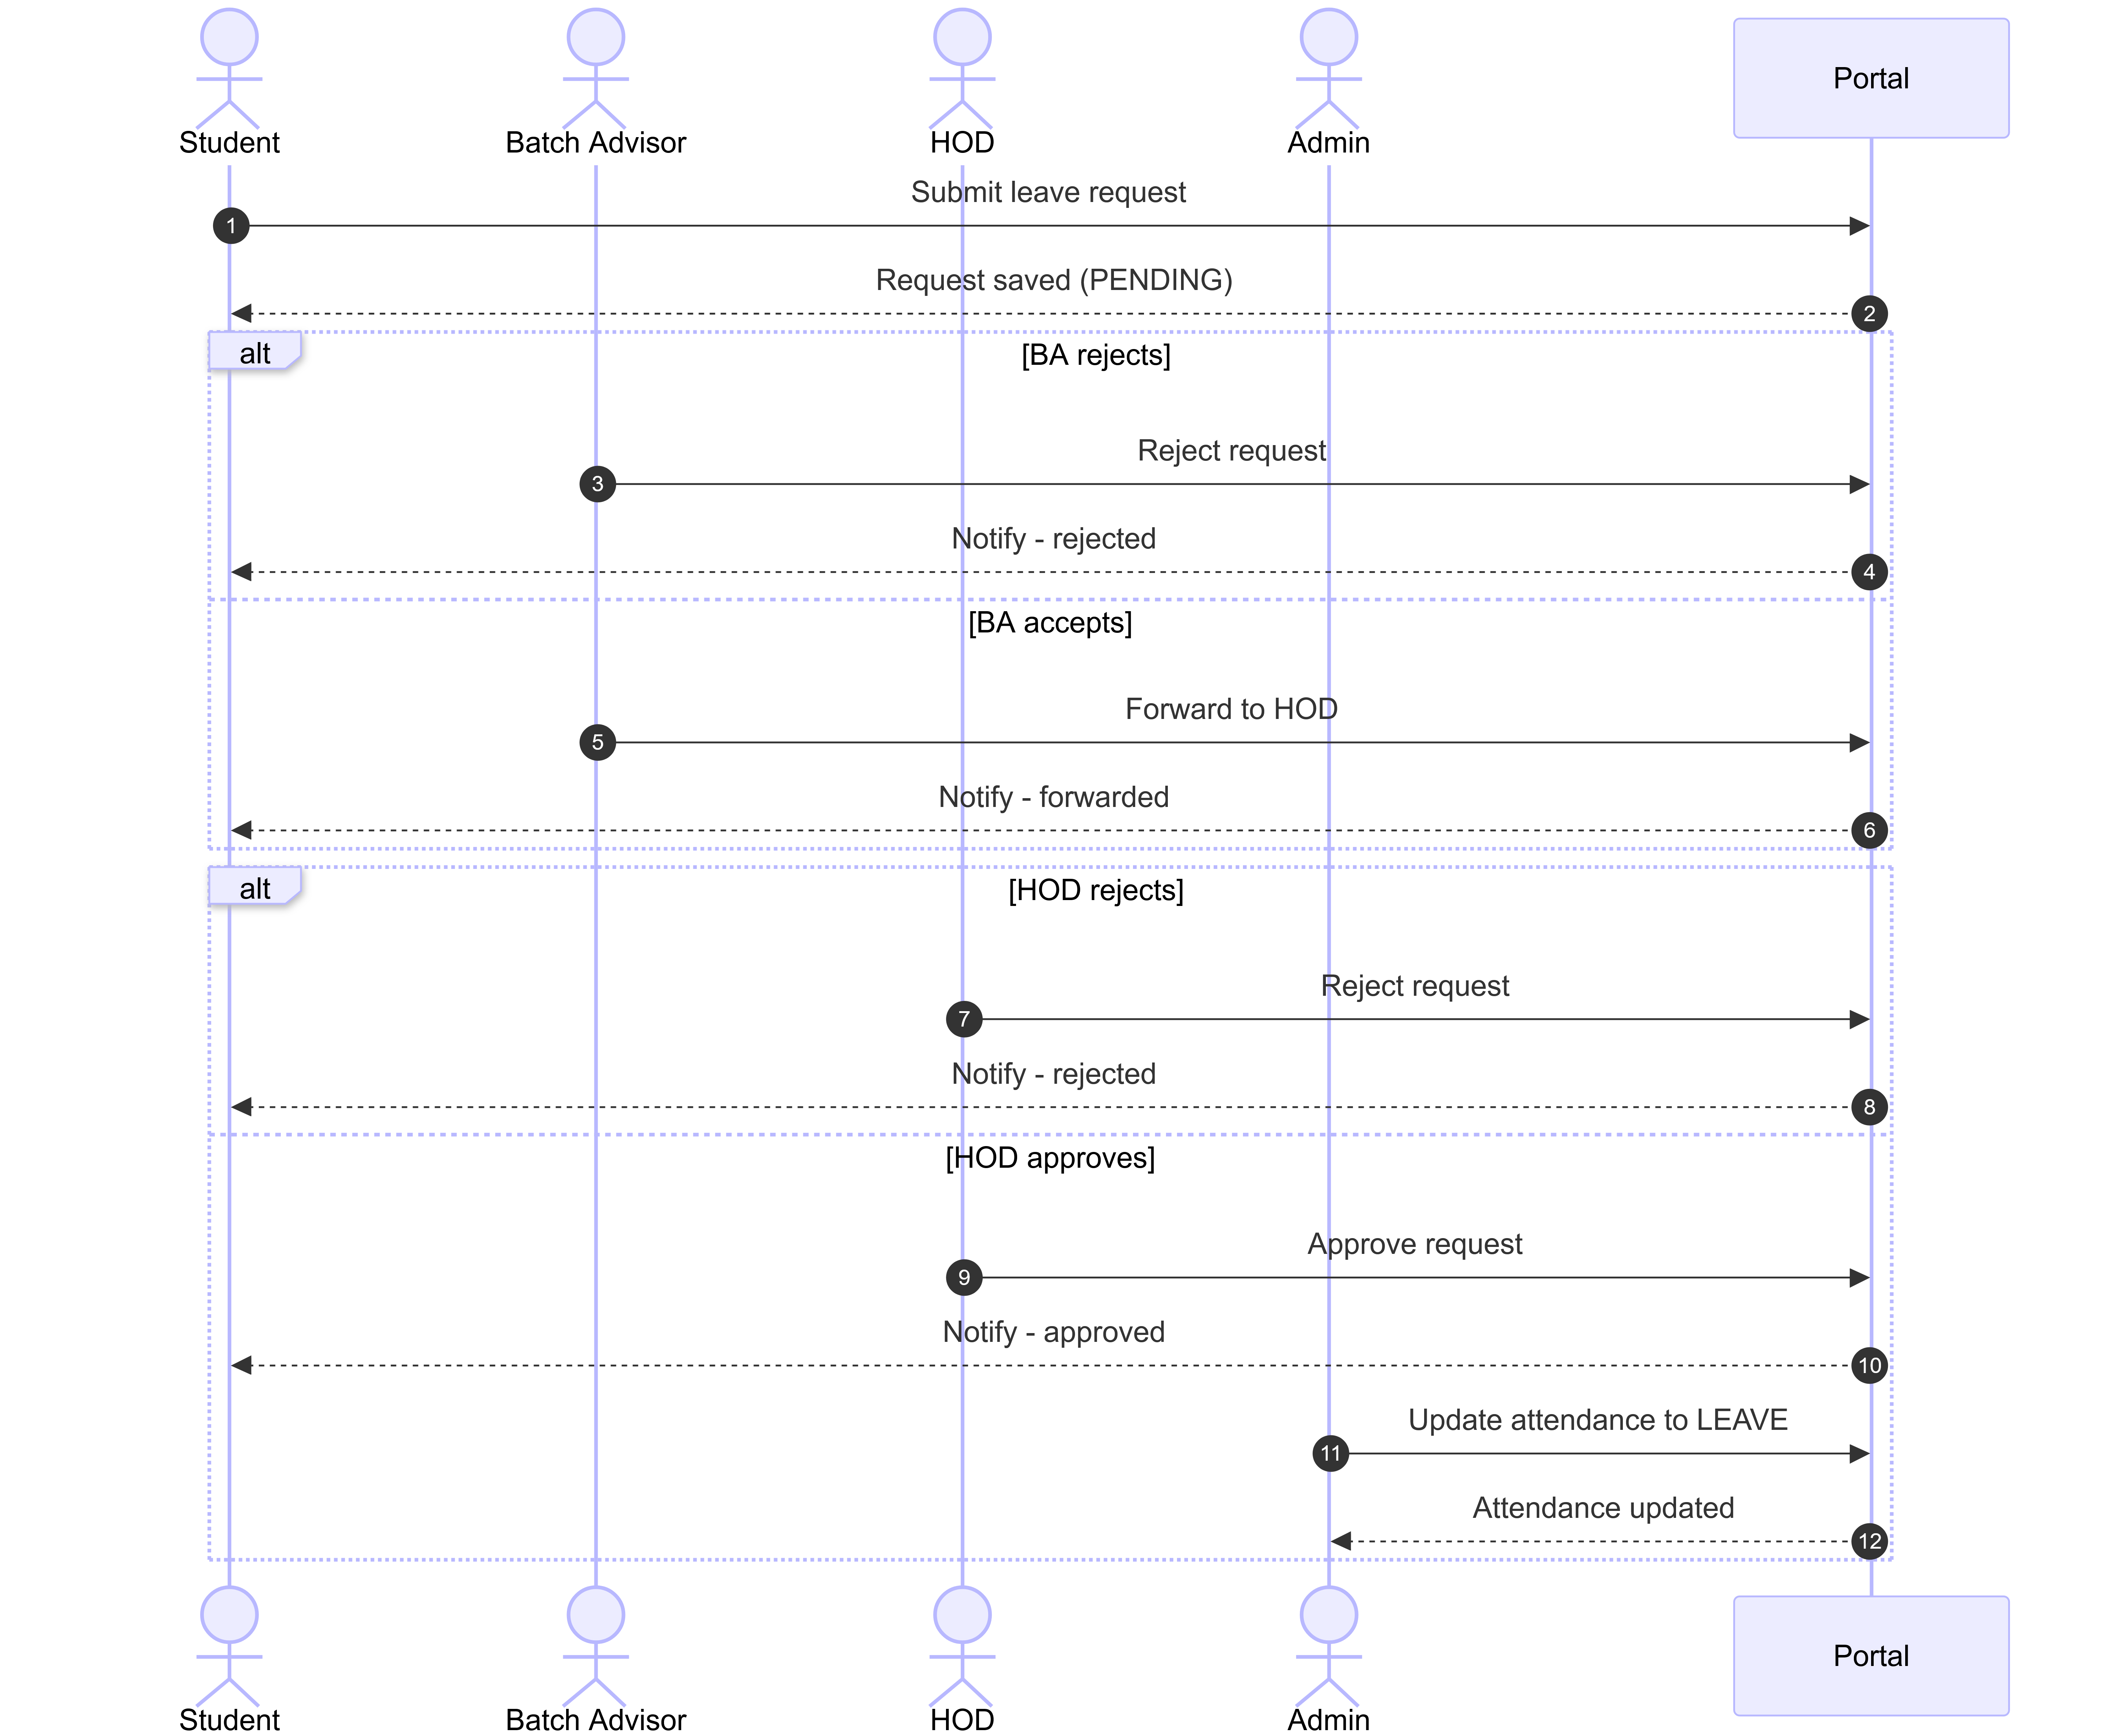
\includegraphics[width=\linewidth]{Figures/diagrams/seq/seq-LR.png}
  \caption{Sequence diagram - Student leave request}
  \label{fig:seq-lr}
\end{figure}

%%%%%%%%%%%%%%%%%%%%%%%%%%%%%%%%%%%%%%%%%%%%%%%%%%%%%%
\subsubsection{Sequence Diagram – Complaint Submission and Resolution Flow}
The complaint process follows a multi-stage review workflow involving the student, BA, and HOD, with support for revision requests, rejection, and reassignment.

\begin{itemize}
    \item Student submits a complaint through the system, providing the category and details.
    \item system acknowledges receipt and sets the complaint status to \texttt{BA\_PENDING}.

    \item BA reviews the complaint:
    \begin{itemize}
        \item On requesting a revision:
        \begin{itemize}
            \item BA requests a revision with remarks via the system. The complaint is not rejected at this stage.
            \item system notifies the student that a revision has been requested.
            \item Student updates the complaint and resubmits through the system.
            \item system notifies the BA that the complaint has been resubmitted for review.
        \end{itemize}
        \item On rejection:
        \begin{itemize}
            \item BA rejects the complaint with remarks on the system.
            \item system notifies the student of the rejection.
        \end{itemize}
        \item On acceptance:
        \begin{itemize}
            \item BA forwards the complaint to the HOD via the system.
            \item system notifies the student that the complaint has been forwarded to the HOD.
        \end{itemize}
    \end{itemize}

    \item HOD reviews the forwarded complaint:
    \begin{itemize}
        \item On rejection:
        \begin{itemize}
            \item HOD rejects the complaint with remarks on the system.
            \item system notifies the student of the rejection.
        \end{itemize}
        \item On resolution:
        \begin{itemize}
            \item HOD marks the complaint as resolved on the system.
            \item system notifies the student that the complaint has been resolved.
        \end{itemize}
        \item On reassignment:
        \begin{itemize}
            \item HOD reassigns the complaint to another department via the system.
            \item system notifies the student that the complaint has been reassigned.
        \end{itemize}
    \end{itemize}
\end{itemize}

\begin{figure}[H]
  \centering
  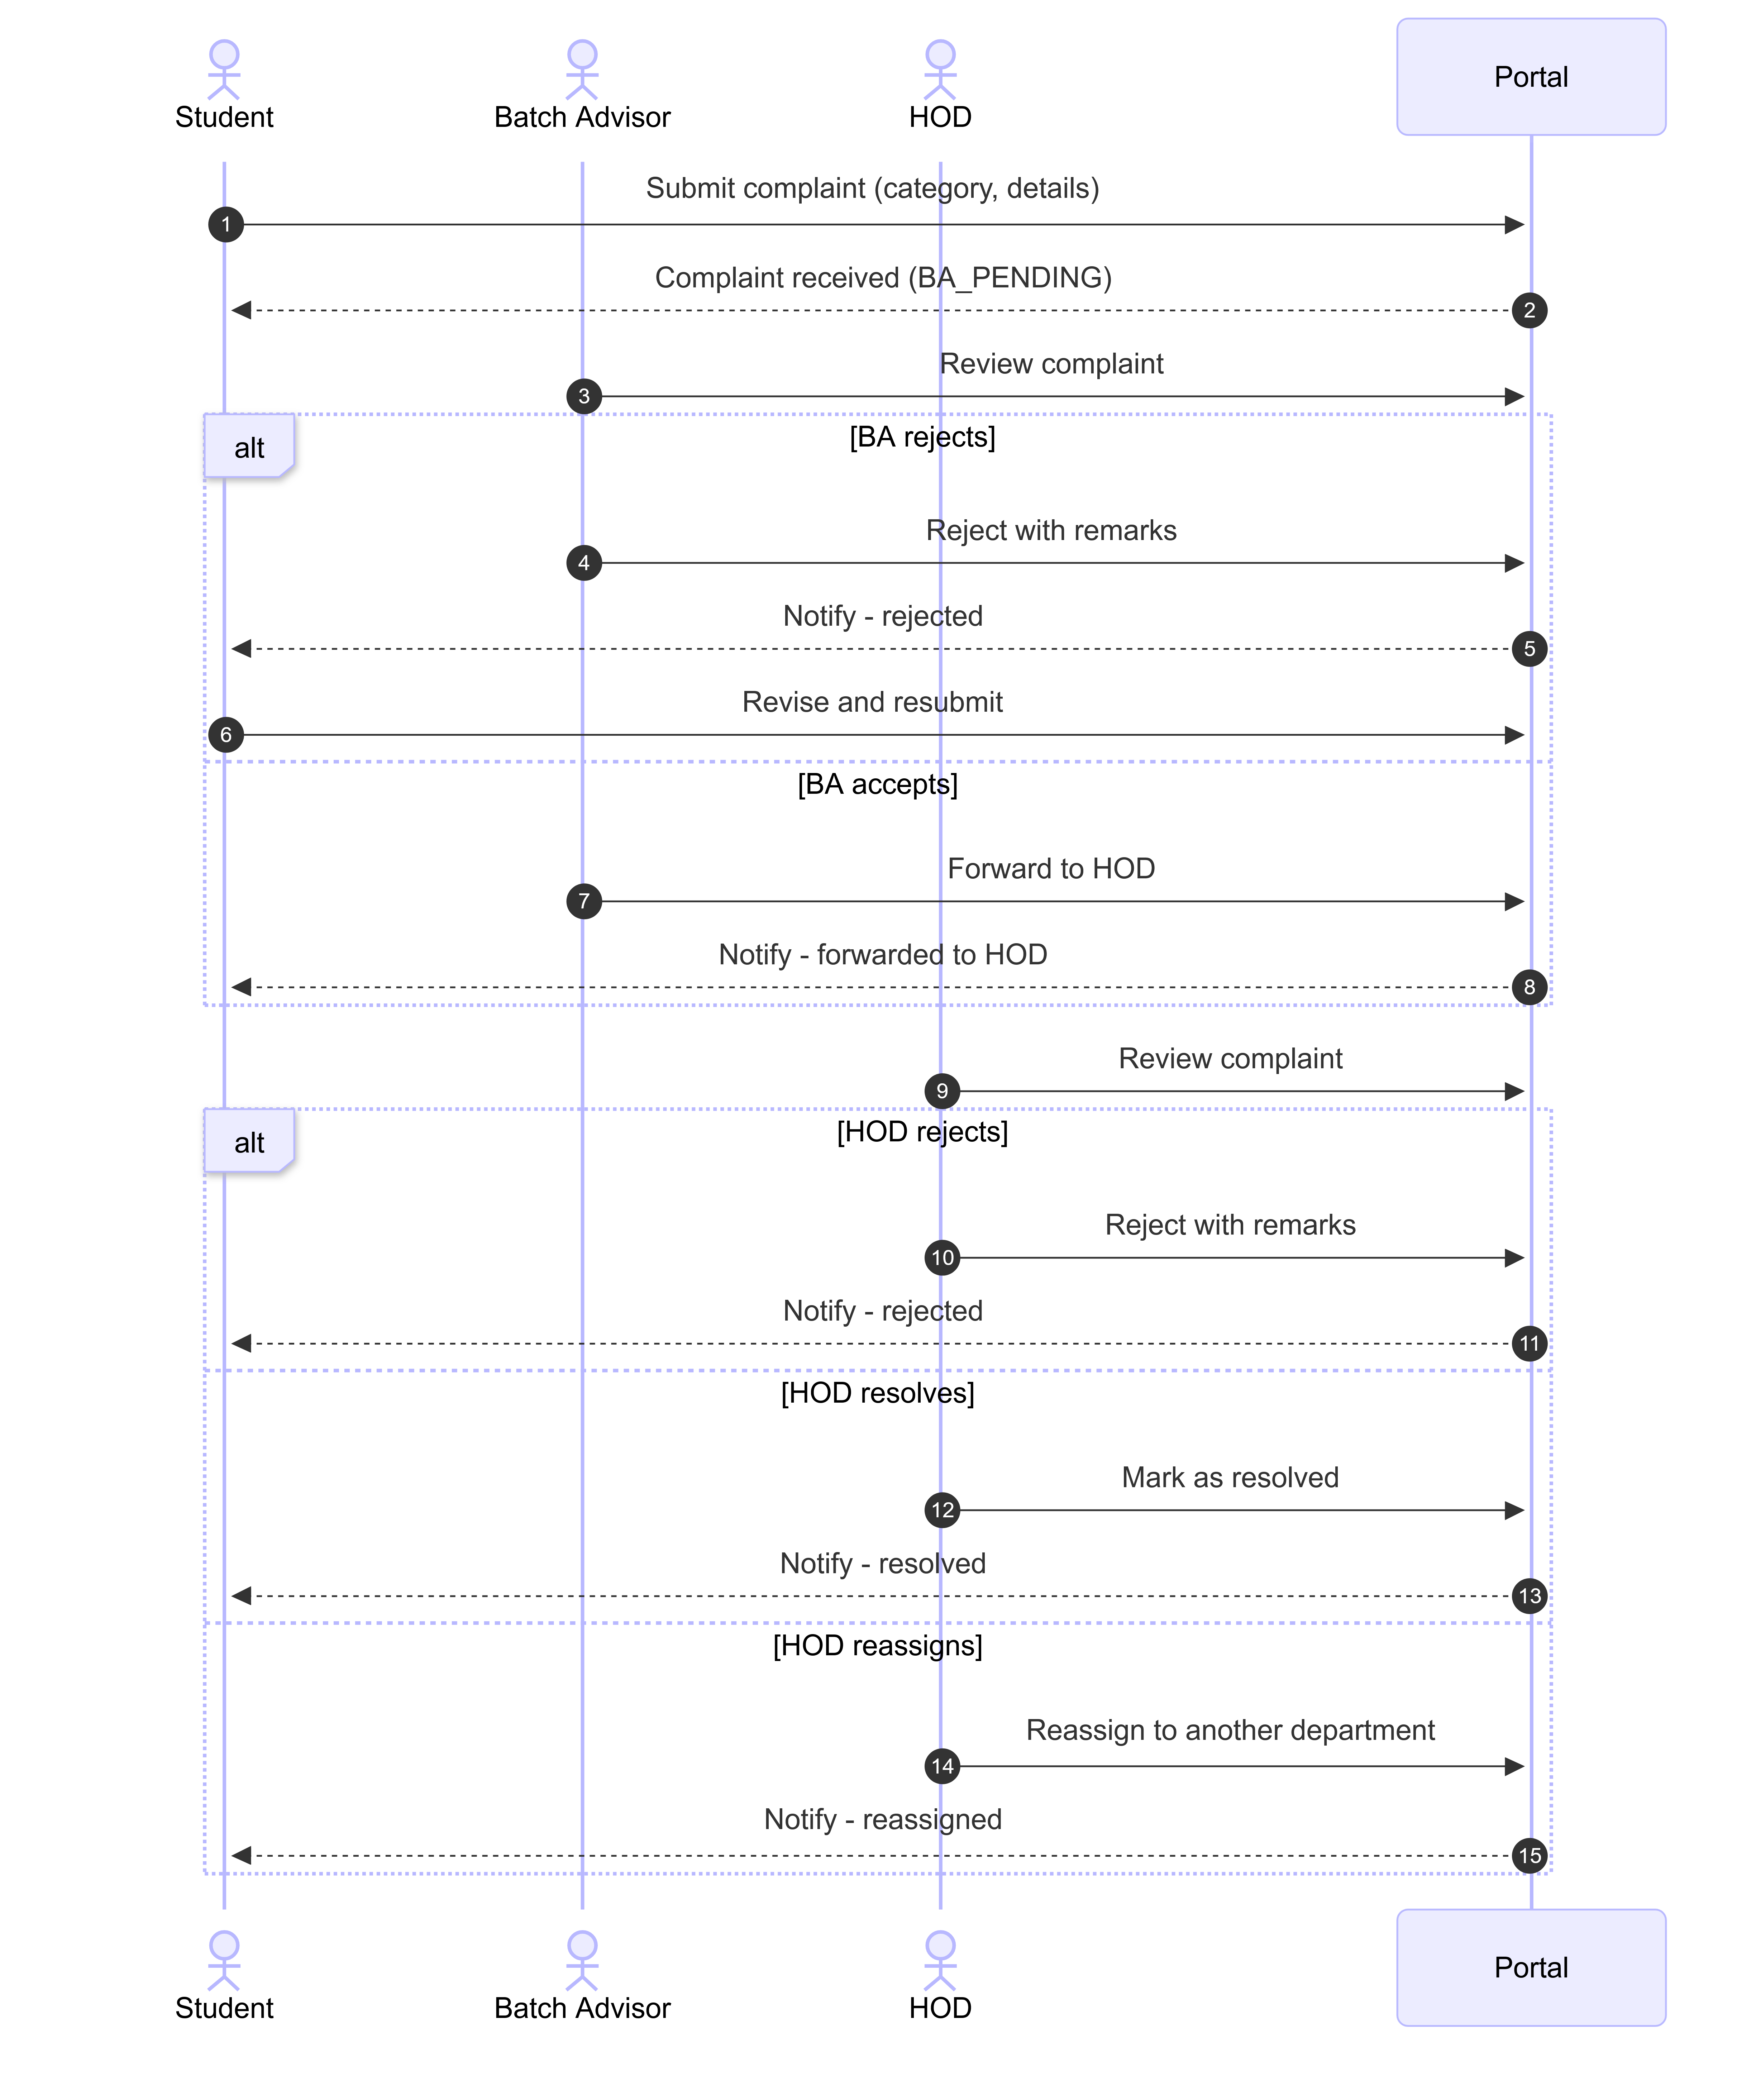
\includegraphics[width=\linewidth]{Figures/diagrams/seq/seq-compl.png}
  \caption{Sequence diagram - Student complaint}
  \label{fig:seq-compl}
\end{figure}

%%%%%%%%%%%%%%%%%%%%%%%%%%%%%%%%%%%%%%%%%%%%%%%%%%%%%%

\subsubsection{Sequence Diagram - Announcement Creation and Scheduling}
The announcement system supports immediate publishing, draft saving, and scheduled publishing via a background job scheduler. Authors with the HOD or Accountant role interact with the system to create and manage announcements.

\begin{itemize}
    \item Author creates an announcement on the system by providing a title, content, and target audience.
    \item system verifies the author's profile against the database before proceeding.
    \item Database confirms the profile, allowing the operation to continue.

    \item Depending on the author's chosen publish option:
    \begin{itemize}
        \item On immediate publishing:
        \begin{itemize}
            \item system inserts the announcement into the database with status \texttt{PUBLISHED}.
            \item system confirms to the author that the announcement is live.
        \end{itemize}
        \item On saving as draft:
        \begin{itemize}
            \item system inserts the announcement into the database with status \texttt{DRAFT}.
            \item system confirms to the author that the draft has been saved.
        \end{itemize}
        \item On scheduling for later:
        \begin{itemize}
            \item system inserts the announcement into the database with status \texttt{SCHEDULED}.
            \item system emits a scheduled event to the Inngest background scheduler.
            \item system confirms to the author that the announcement has been scheduled.
            \item Inngest sleeps until the specified \texttt{scheduledFor} datetime is reached.
            \item Once triggered, Inngest updates the announcement status in the database to \texttt{PUBLISHED}.
        \end{itemize}
    \end{itemize}

    \item Author views the announcement feed on the system.
    \item system queries the database for all \texttt{PUBLISHED} announcements filtered by the author's audience scope.
    \item Database returns the matching announcement list to the system.
    \item system renders the feed and displays it to the author.
\end{itemize}

\begin{figure}[H]
  \centering
  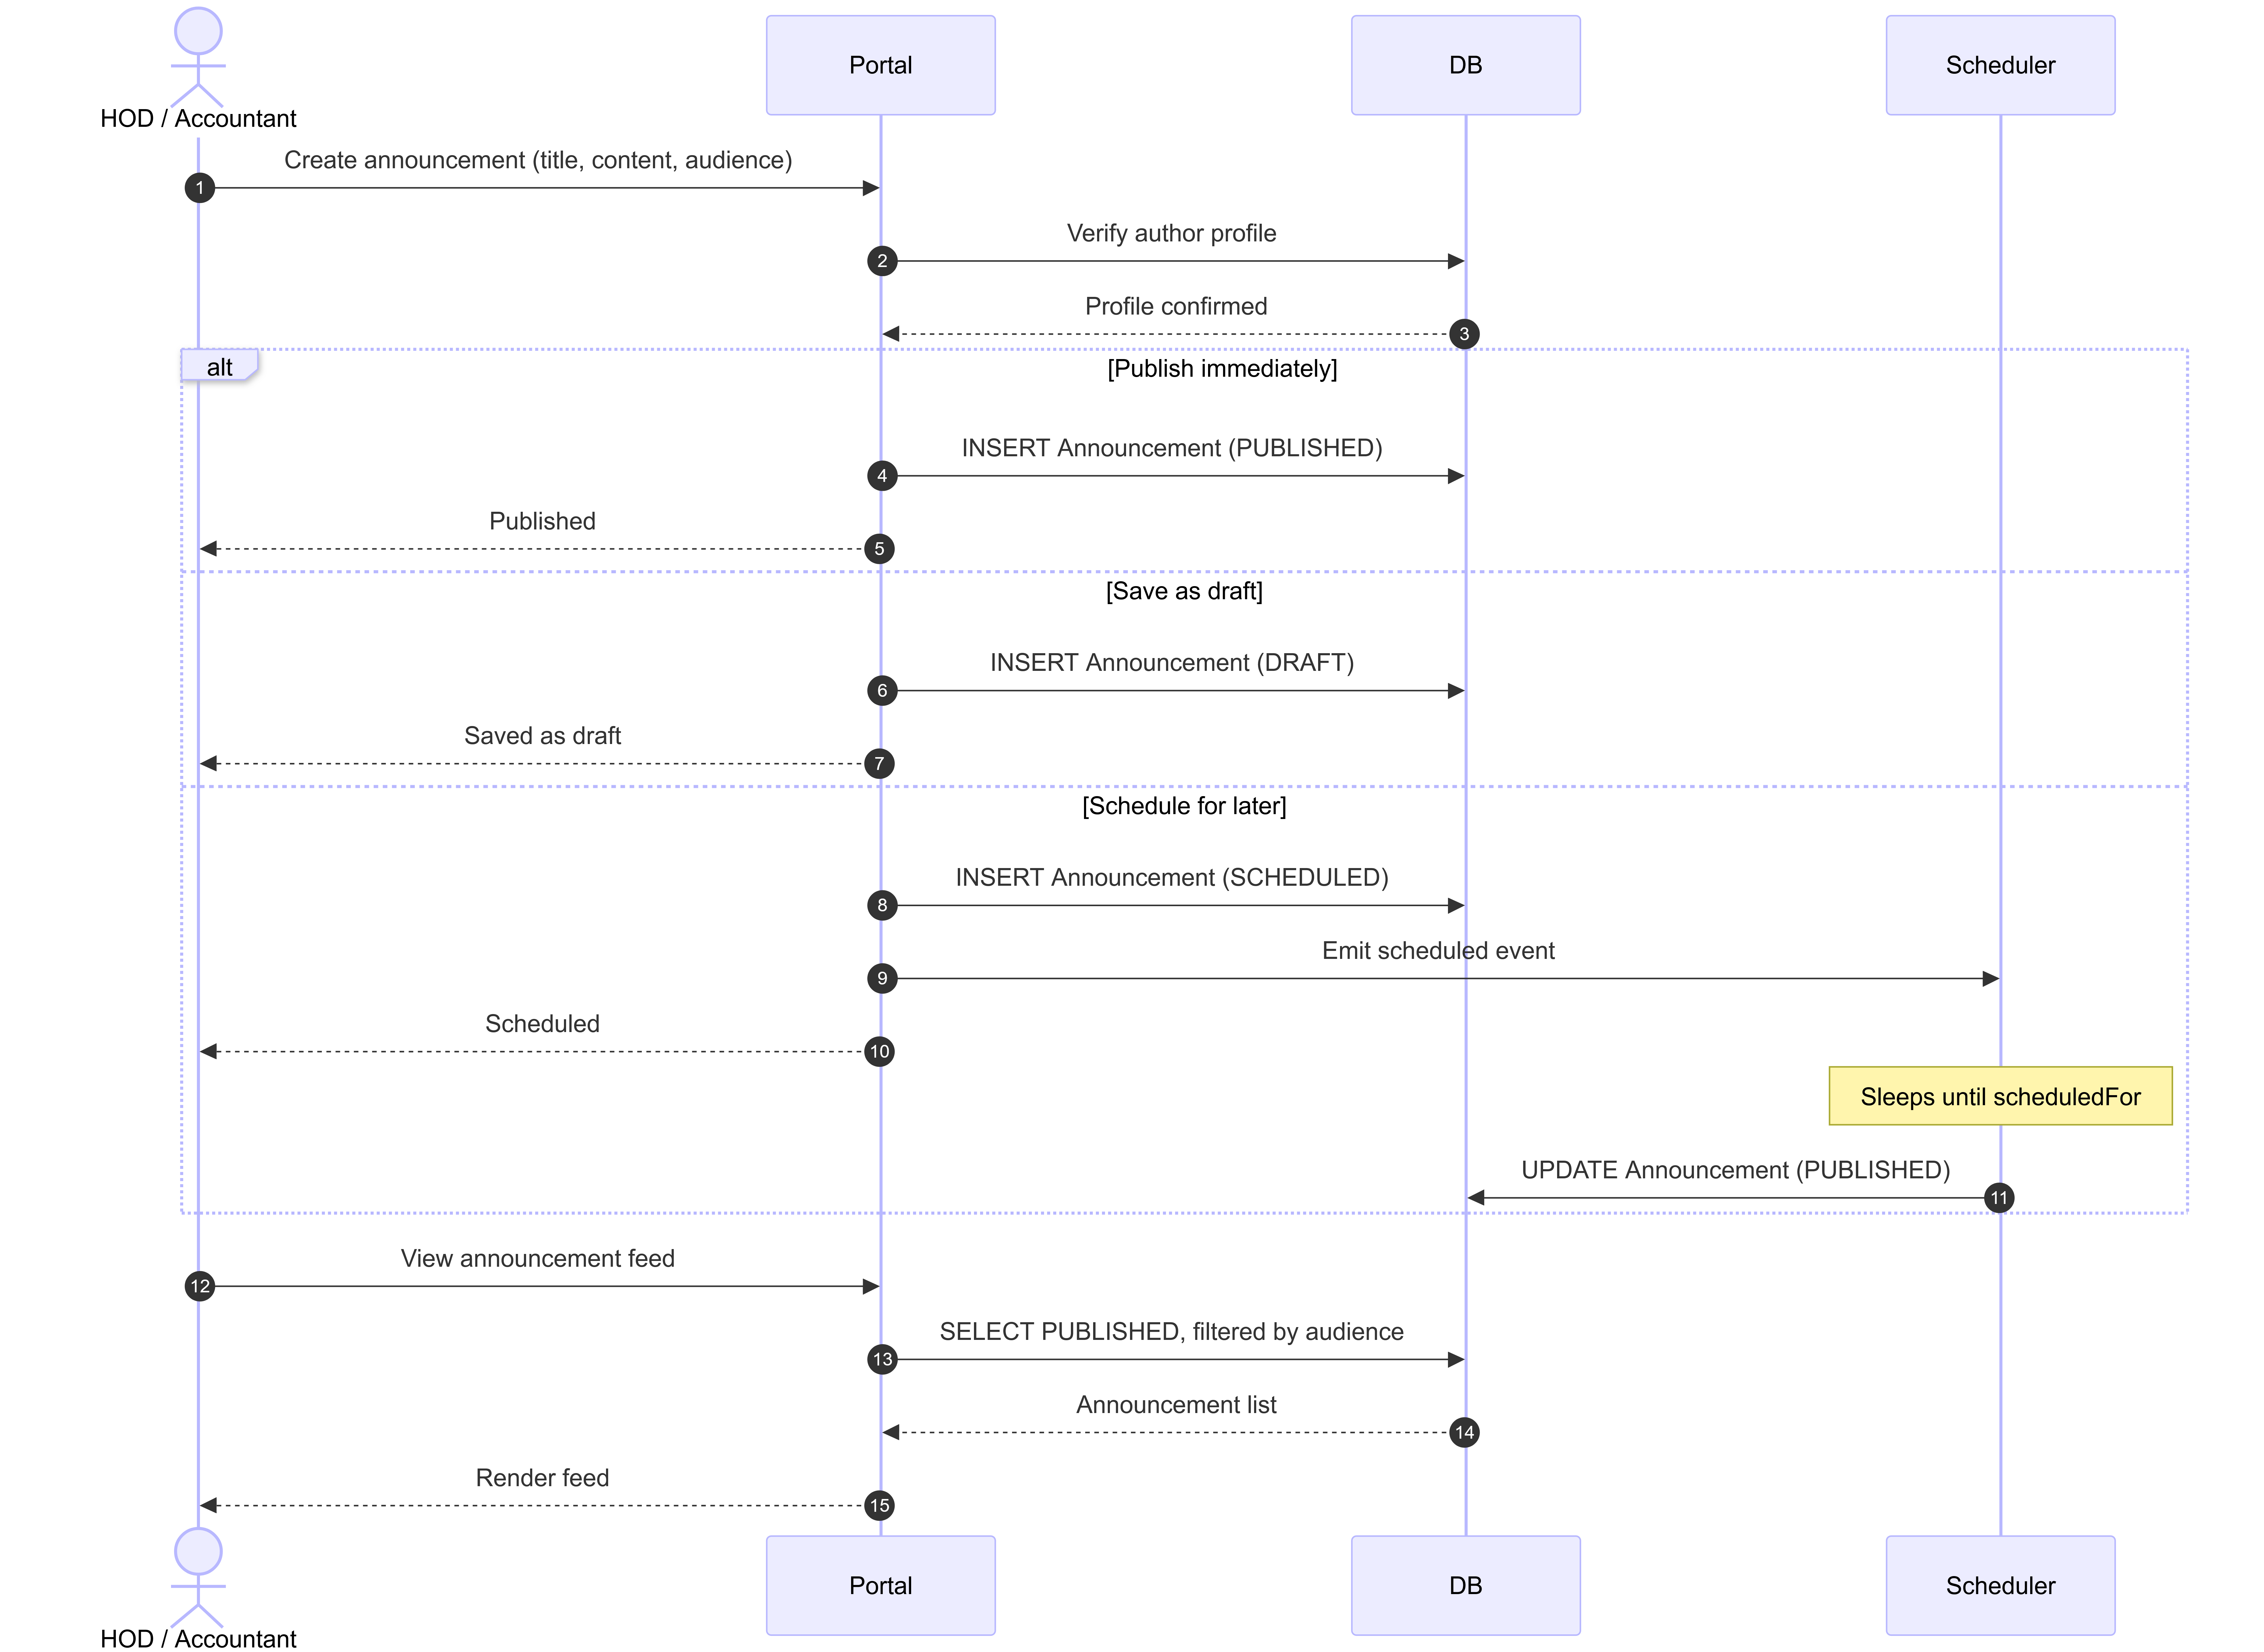
\includegraphics[width=\linewidth]{Figures/diagrams/seq/seq-ann.png}
  \caption{Sequence diagram - Announcement}
  \label{fig:seq-ann}
\end{figure}

%%%%%%%%%%%%%%%%%%%%%%%%%%%%%%%%%%%%%%%%%%%%%%%%%%%%%%
\subsection{State Transition Diagrams}

State diagrams show how system or object changes states over time.

\subsubsection{Leave request - State Transition:}

A LR passes through five distinct states before it reaches a terminal
outcome. The full life-cycle is driven by two sequential reviewers — the BA and the HOD. If accepted by BA and HOD, admin can update students attendance.

\textbf{States}

\begin{tabular}{ll}
\toprule
\textbf{State}            & \textbf{Description} \\
\midrule
\texttt{PENDING}          & Request submitted, awaiting BA review \\
\texttt{REVIEW\_REQUESTED} & BA requested clarification / more details \\
\texttt{HOD\_PENDING}     & BA accepted → awaiting HOD final decision \\
\texttt{APPROVED}         & Leave approved (terminal state) \\
\texttt{REJECTED}         & Leave rejected (terminal state) \\
\bottomrule
\end{tabular}

\textbf{State Transitions}

\begin{itemize}
  \item Student submits leave request
    $\rightarrow$ status = \texttt{PENDING} (Department auto-set from student's profile)

  \item While \texttt{PENDING}:
    \begin{itemize}
      \item Student can edit form or delete permanently
      \item BA can:
        \begin{itemize}
          \item Request update/more info $\rightarrow$ \texttt{REVIEW\_REQUESTED}
                + remarks saved
          \item Reject $\rightarrow$ \texttt{REJECTED}
                + remarks saved (terminal)
          \item Accept $\rightarrow$ \texttt{HOD\_PENDING}
                + remarks (optional)
        \end{itemize}
    \end{itemize}

  \item While \texttt{REVIEW\_REQUESTED}:
    \begin{itemize}
      \item Student updates form and resubmits
        $\rightarrow$ status resets to \texttt{PENDING}
      \item Student can still delete
    \end{itemize}

  \item While \texttt{HOD\_PENDING}:
    \begin{itemize}
      \item HOD can:
        \begin{itemize}
          \item Reject $\rightarrow$ \texttt{REJECTED}
                + remarks saved (terminal)
          \item Accept $\rightarrow$ \texttt{APPROVED}
                + remarks (optional) (terminal)
        \end{itemize}
    \end{itemize}


  \item Terminal states:
    \begin{itemize}
      \item \texttt{APPROVED} $\quad\Rightarrow$ leave approved, attendance updated
      \item \texttt{REJECTED} $\quad\Rightarrow$ leave denied, no further action
    \end{itemize}
\end{itemize}


\begin{figure}[H]
  \centering
  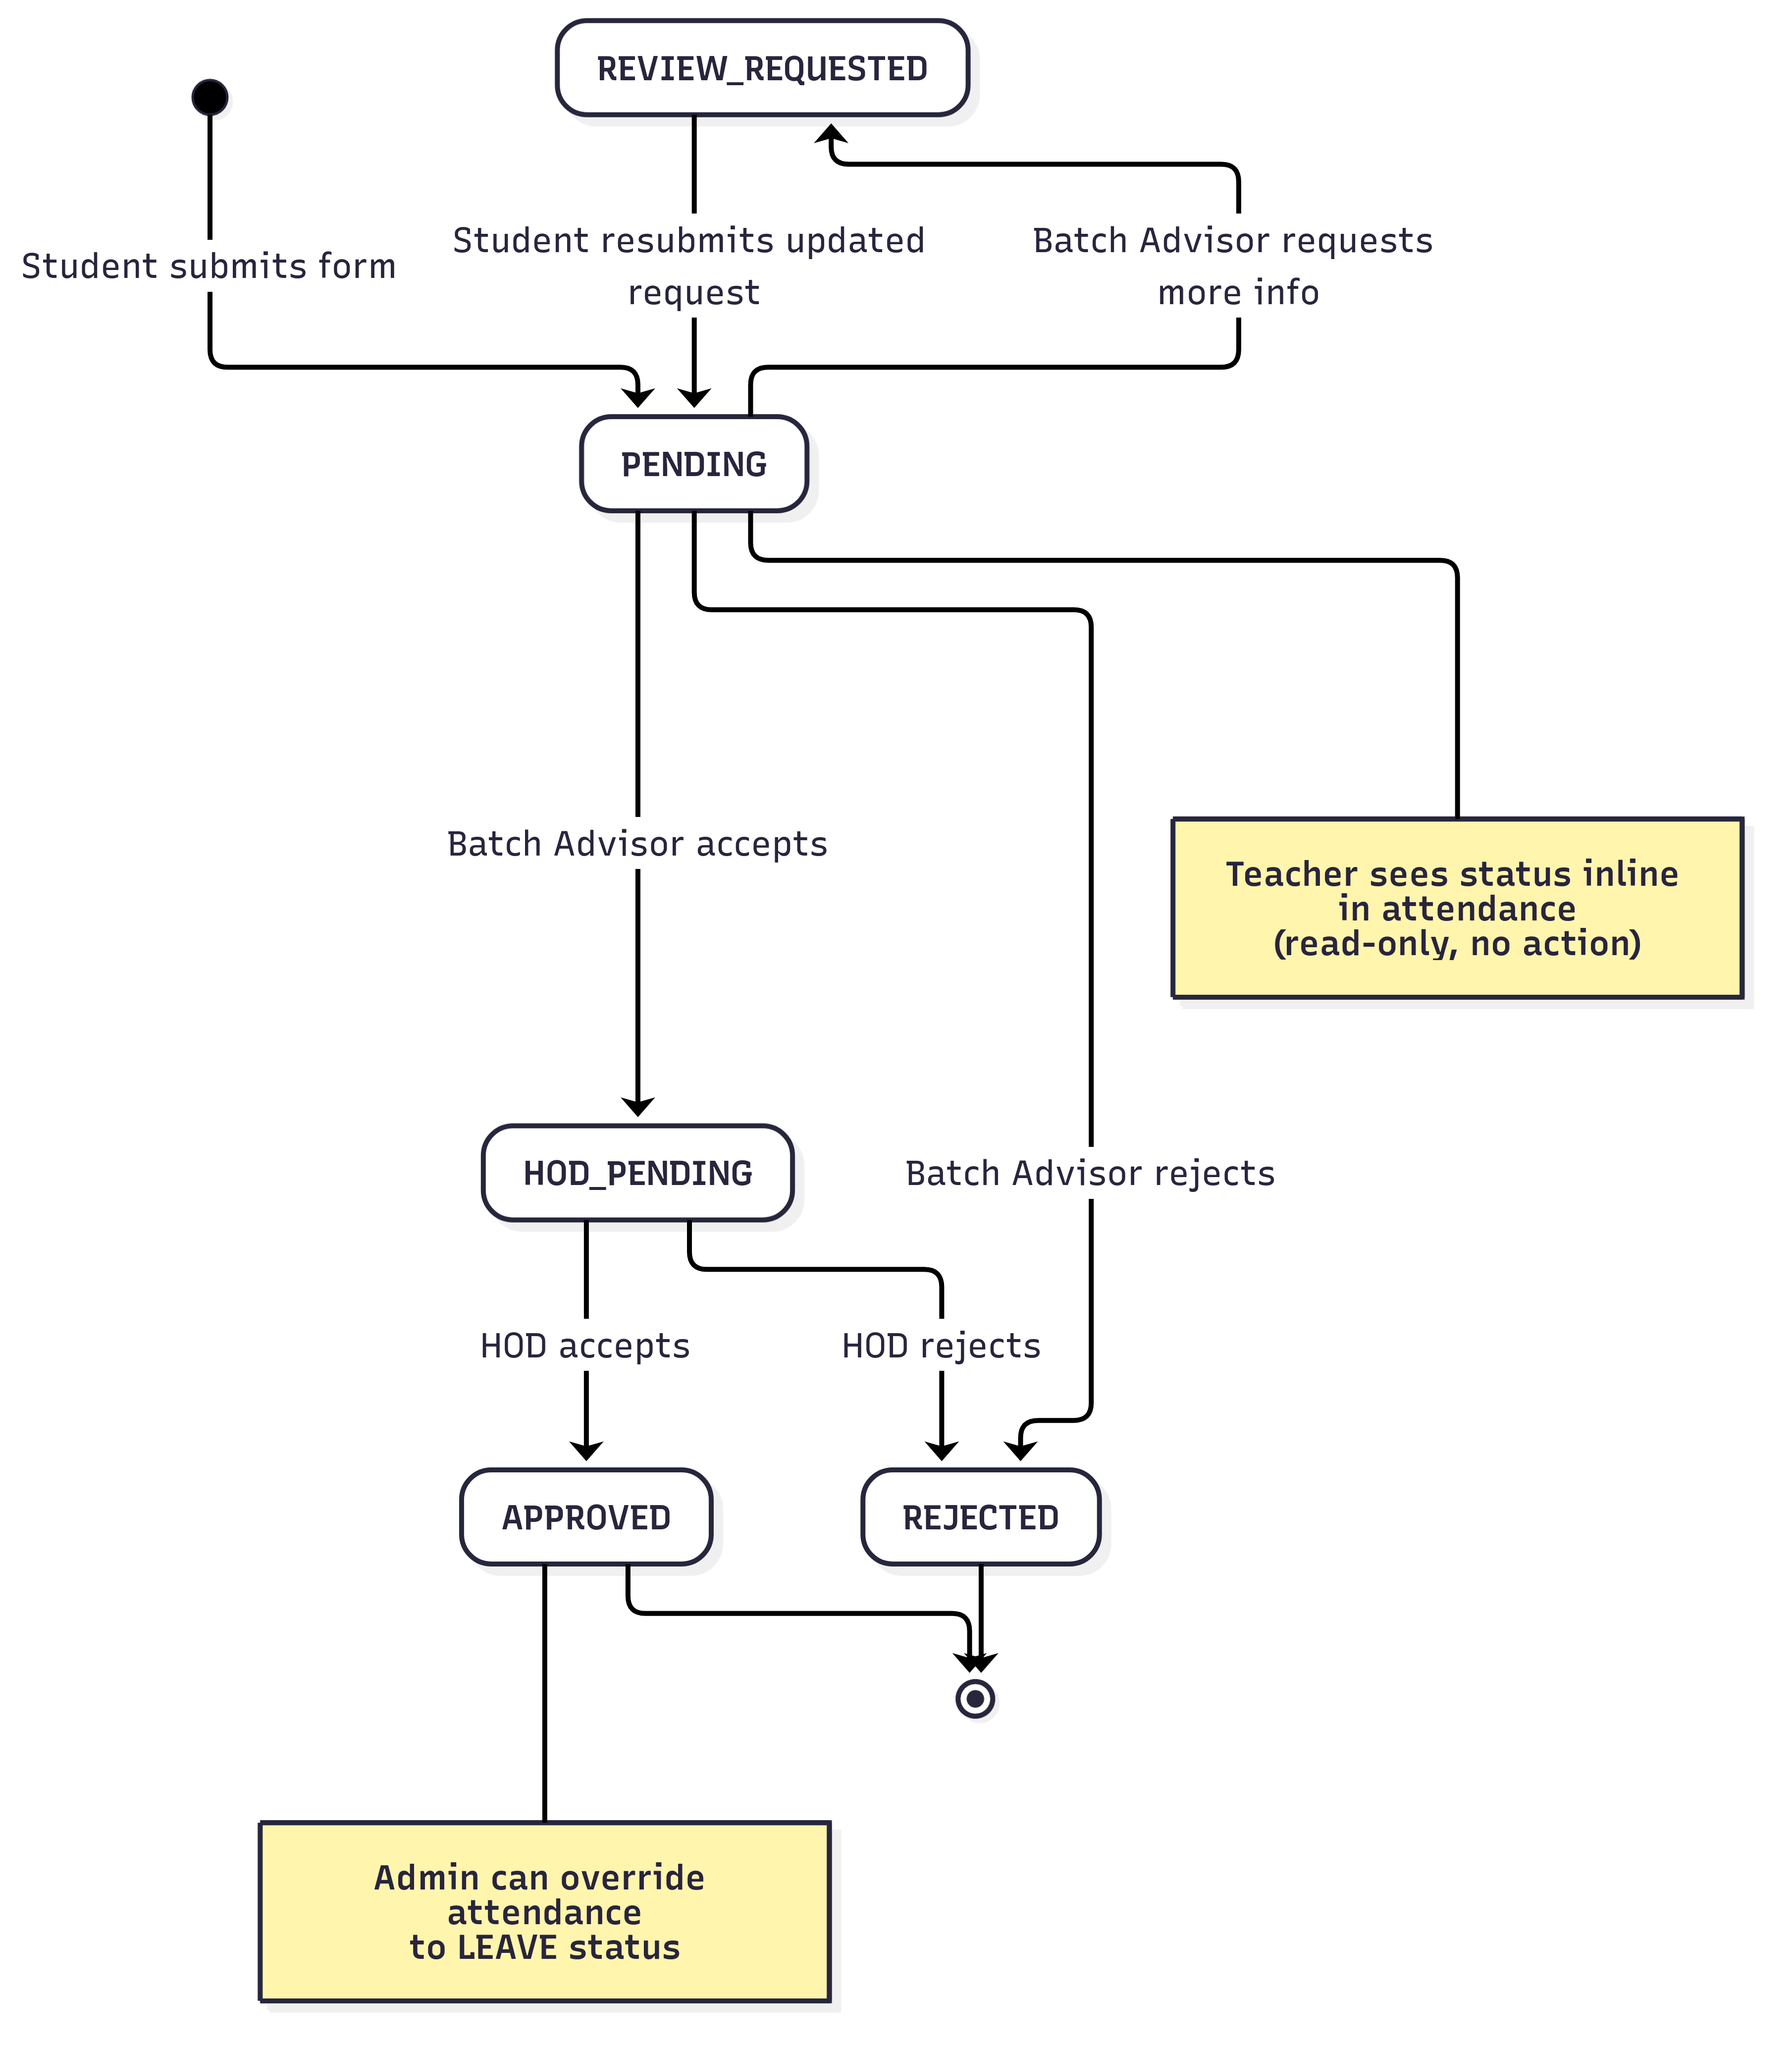
\includegraphics[width=\linewidth]{Figures/diagrams/state/st-lr1.png}
  \caption{State transition - Leave request}
  \label{fig:st-lr}
\end{figure}

%%%%%%%%%%%%%%%%%%%%%%%%%%%%%%%%%%%%%%%%%%%%%%%%%%%%%%%%%%%%%%
%%%%%%%%%%%%%%%%%%%%%%%%%%%%%%%%%%%%%%%%%%%%%%%%%%%%%%%%%%%%%%

\subsubsection{Complaint - State Transition}


\textbf{States:}

\begin{itemize}
  \item \textbf{BA\_PENDING} \quad initial state after student submission
  \item \textbf{BA\_REVIEW\_REQUESTED} \quad BA needs more details
  \item \textbf{BA\_REJECTED} \quad rejected by BA (student can update details)
  \item \textbf{HOD\_PENDING} \quad escalated — awaiting HOD decision
  \item \textbf{HOD\_ACCEPTED} \quad resolved / accepted by HOD (terminal)
  \item \textbf{HOD\_REJECTED} \quad rejected by HOD (terminal)
  \item \textbf{ASSIGNED} \quad HOD assigned to another department (terminal)
\end{itemize}

\textbf{Transitions}

\begin{itemize}
  \item \textbf{Student submits} $\to$ \texttt{BA\_PENDING}
        \quad Department set from student profile

  \item \textbf{Student edits} \quad \texttt{BA\_PENDING} $\to$ \texttt{BA\_PENDING}
        \quad content updated, \texttt{ComplaintReview} entry written

  \item \textbf{BA requests more info} \quad \texttt{BA\_PENDING} $\to$ \texttt{BA\_REVIEW\_REQUESTED}
        \quad remarks saved, student notified

  \item \textbf{Student resubmits (BA stage)} \quad \texttt{BA\_REVIEW\_REQUESTED} $\to$ \texttt{BA\_PENDING}
        \quad updated content, \texttt{ComplaintReview} entry created, re-enters BA queue

  \item \textbf{BA accepts} \quad \texttt{BA\_PENDING} $\to$ \texttt{HOD\_PENDING}
        \quad remarks saved, \texttt{ComplaintReview} entry written, student notified

  \item \textbf{BA rejects} \quad \texttt{BA\_PENDING} $\to$ \texttt{BA\_REJECTED}
        \quad remarks saved, \texttt{ComplaintReview} entry written, student notified

  \item \textbf{Student revises after rejection} \quad \texttt{BA\_REJECTED} $\to$ \texttt{BA\_PENDING}
        \quad new \texttt{ComplaintReview} entry created

  \item \textbf{Student deletes} \quad \texttt{BA\_PENDING} / \texttt{BA\_REVIEW\_REQUESTED} / \texttt{BA\_REJECTED} $\to$ [*]
        \quad permanent removal + cascade delete of reviews \& assignments

  \item \textbf{HOD accepts} \quad \texttt{HOD\_PENDING} $\to$ \texttt{HOD\_ACCEPTED}
        \quad remarks saved, \texttt{ComplaintReview} entry written, student notified (resolved)

  \item \textbf{HOD rejects} \quad \texttt{HOD\_PENDING} $\to$ \texttt{HOD\_REJECTED}
        \quad remarks saved, \texttt{ComplaintReview} entry written, student notified (workflow ends)

  \item \textbf{HOD assigns} \quad \texttt{HOD\_PENDING} $\to$ \texttt{ASSIGNED}
        \quad new target department + reason, \texttt{targetDepartment} updated
        \quad transaction writes: Complaint update → ASSIGNED, \texttt{ComplaintAssignment} log, \texttt{ComplaintReview} entry
        \quad complaint terminal in assigned state, receiving department sees as assignment notification
\end{itemize}
 
\begin{figure}[H]
  \centering
  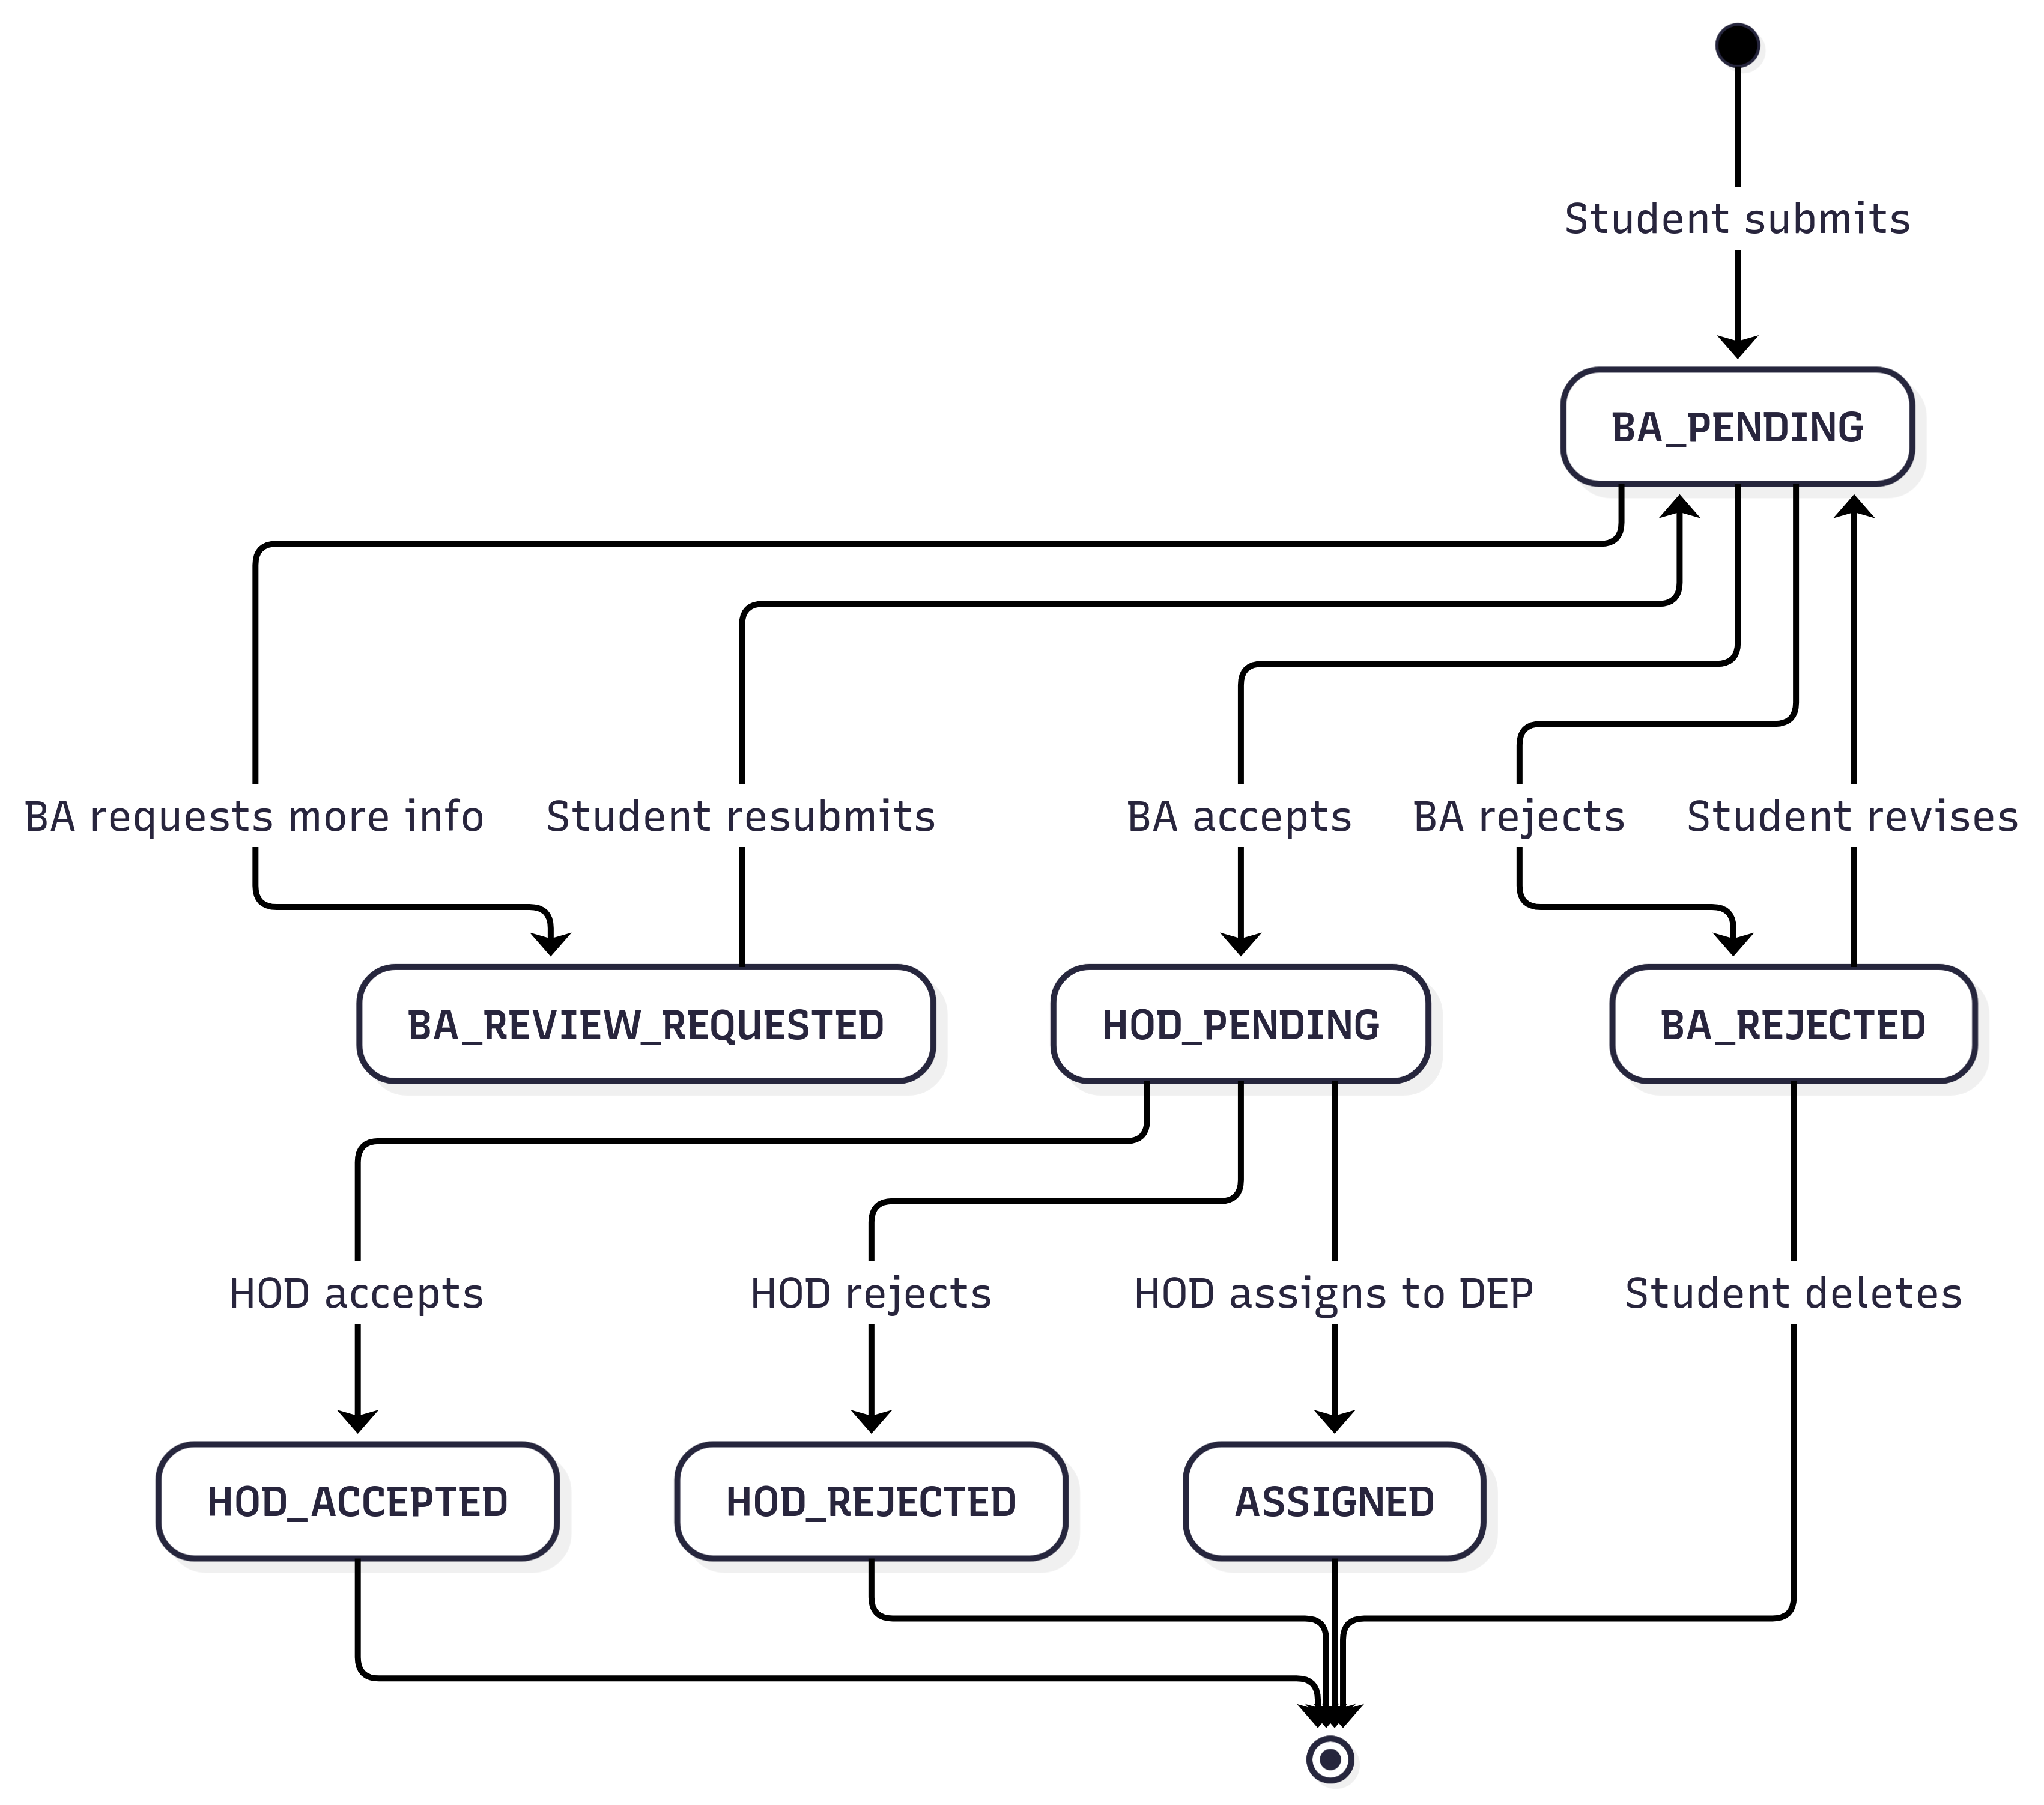
\includegraphics[width=\linewidth]{Figures/diagrams/state/st-compl.png}
  \caption{State transition - Complaint}
  \label{fig:st-compl}
\end{figure}


%%%%%%%%%%%%%%%%%%%%%%%%%%%%%%%%%%%%%%%%%%%%%%%%%%%%%%%%%%%%%%


\subsubsection{Announcement - State Transition}


\textbf{Flow:}

\begin{itemize}
  \item Author creates announcement and lands in \texttt{DRAFT}.
  \item From \texttt{DRAFT}, author can publish now, schedule for later, or delete.
  \item If \texttt{SCHEDULED}, a background job publishes automatically at \texttt{scheduledFor}.
  \item Students only see \texttt{PUBLISHED} announcements (filtered by audience scope).
  \item Published announcements can be archived and later restored.
\end{itemize}

\textbf{States:}

\begin{itemize}
  \item \textbf{DRAFT} \quad saved, not visible to students
  \item \textbf{SCHEDULED} \quad queued for future publish
  \item \textbf{PUBLISHED} \quad visible to students
\end{itemize}

\textbf{Transitions:}

\begin{itemize}
  \item \textbf{Save draft} $\to$ \texttt{DRAFT}
  \item \textbf{Publish now} \quad \texttt{DRAFT} $\to$ \texttt{PUBLISHED}
  \item \textbf{Schedule} \quad \texttt{DRAFT} $\to$ \texttt{SCHEDULED}
  \item \textbf{Auto publish} \quad \texttt{SCHEDULED} $\to$ \texttt{PUBLISHED}
  \item \textbf{Cancel schedule} \quad \texttt{SCHEDULED} $\to$ \texttt{DRAFT}
  \item \textbf{Delete} \quad any active state $\to$ [*]
\end{itemize}

\begin{figure}[H]
  \centering
  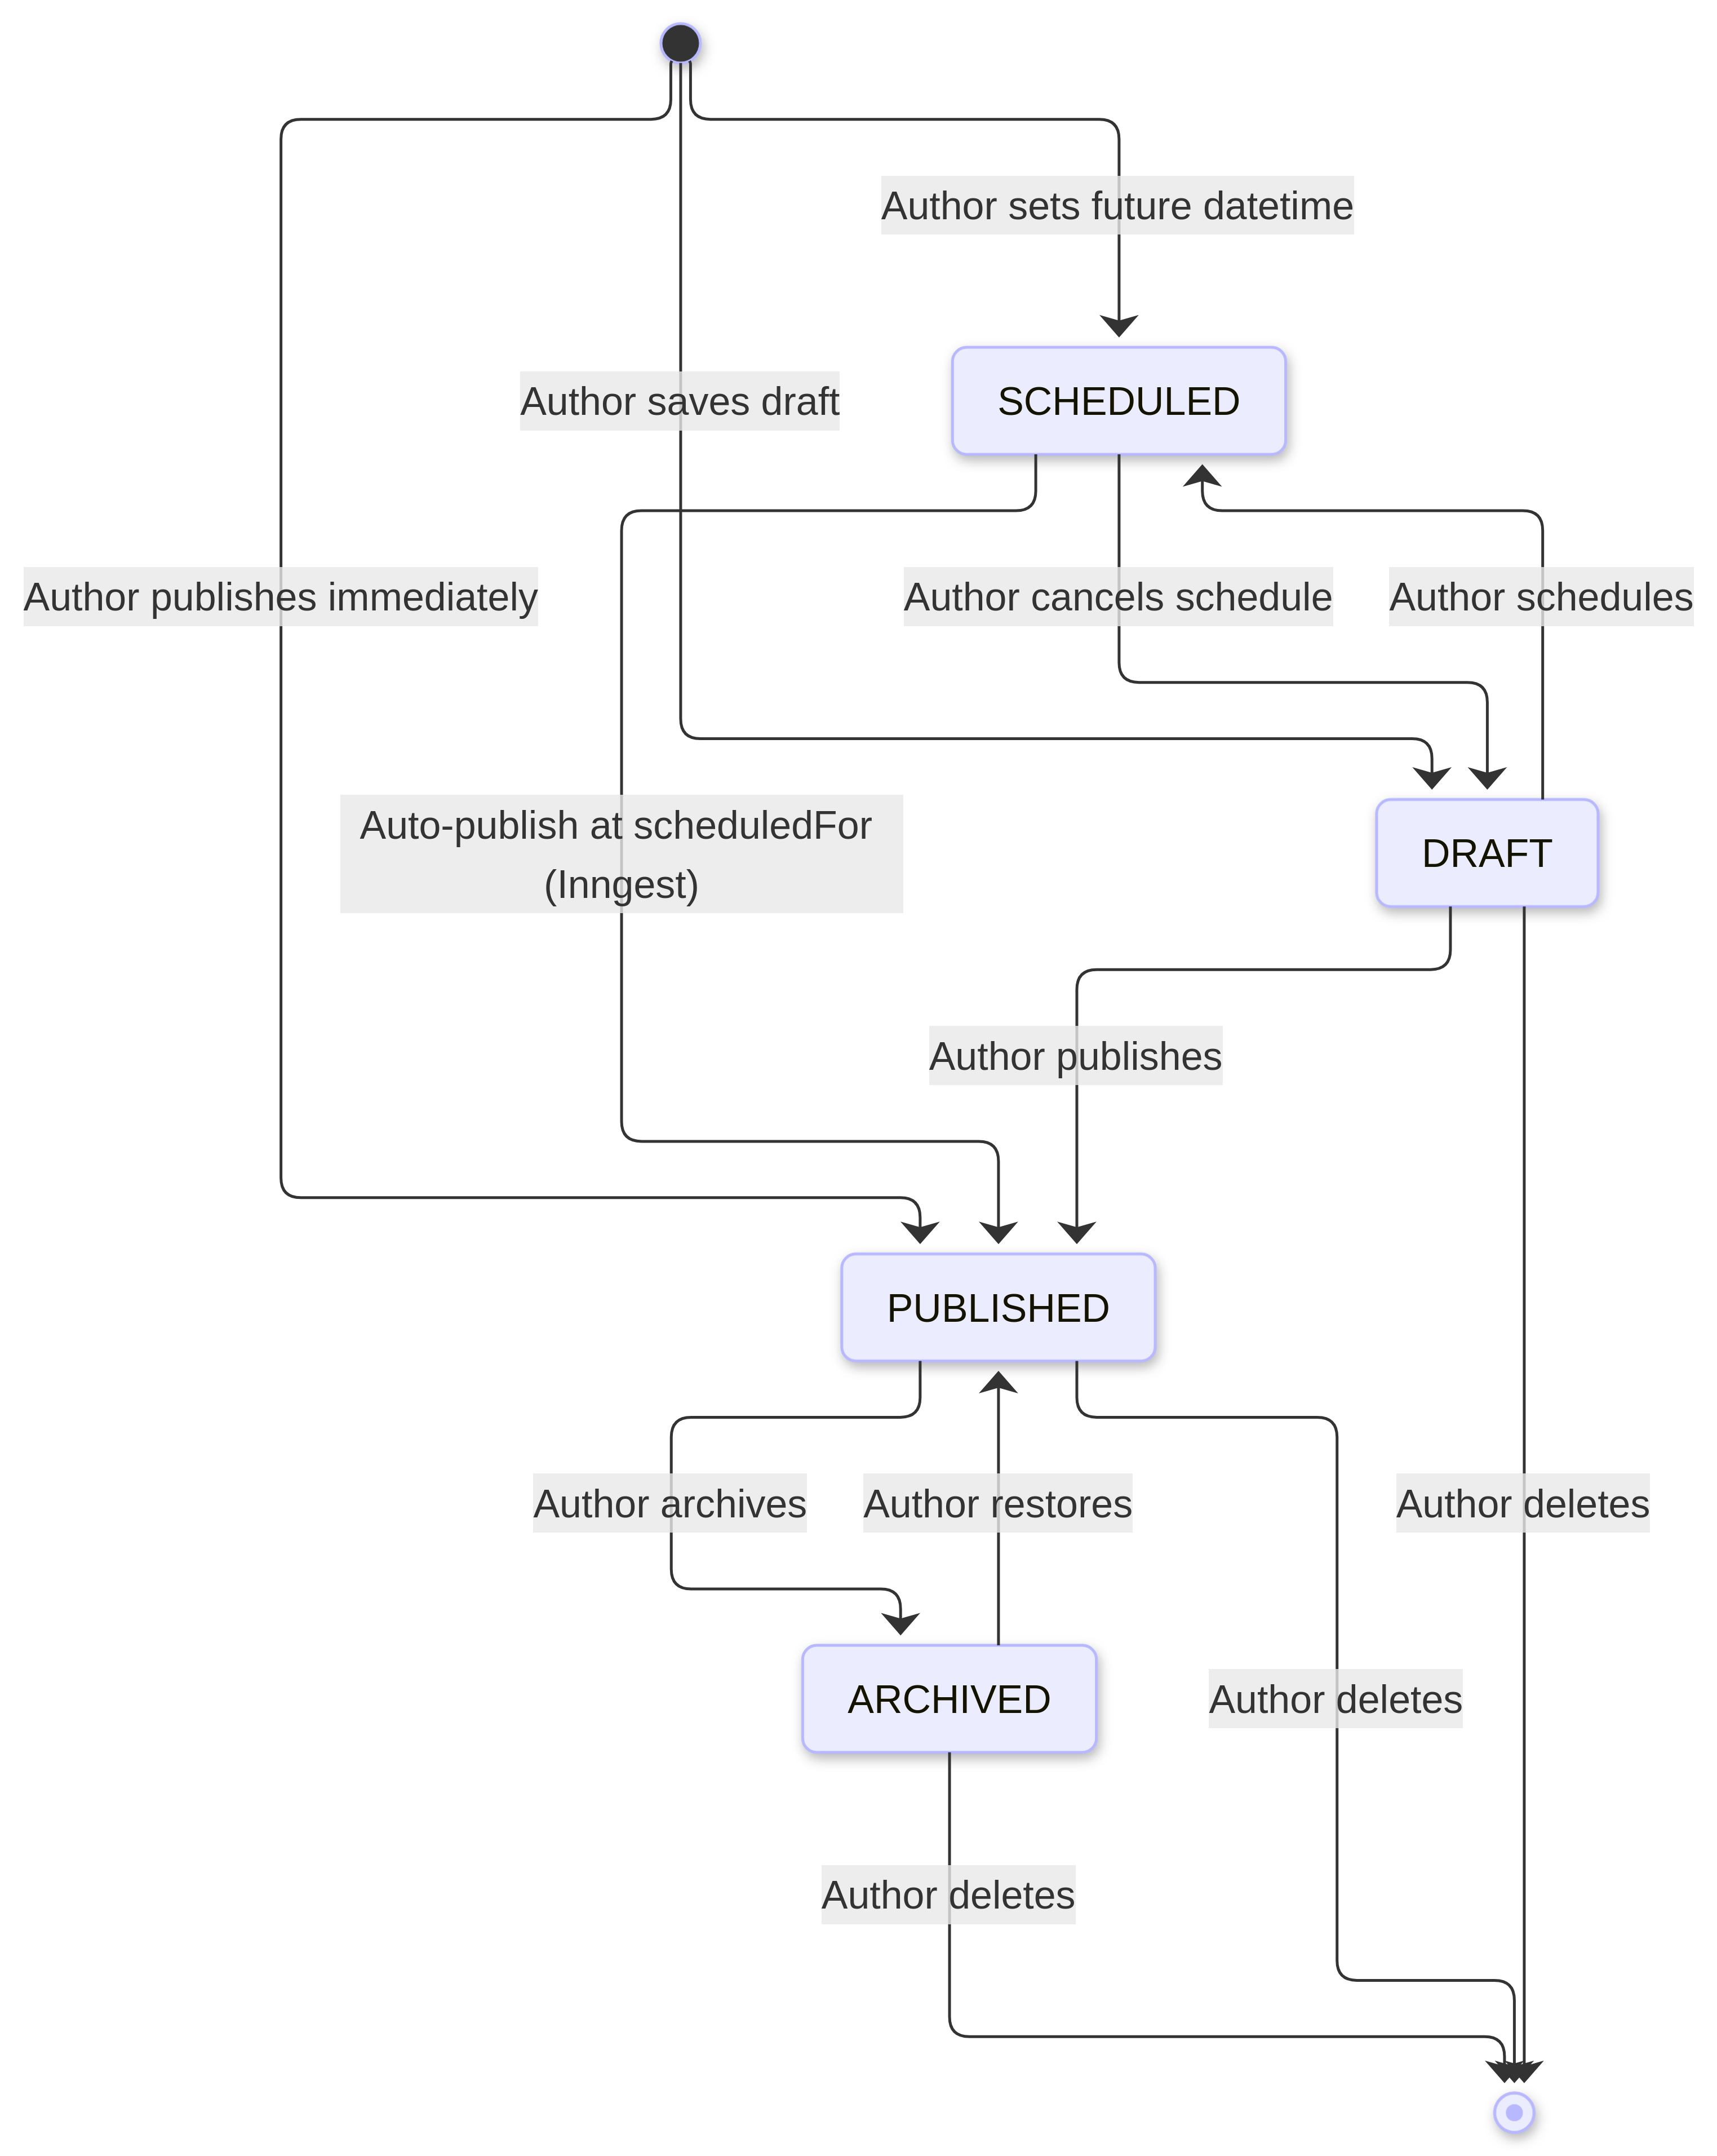
\includegraphics[width=\linewidth]{Figures/diagrams/state/st-ann.png}
  \caption{State transition - Announcement}
  \label{fig:st-ann}
\end{figure}


%%%%%%%%%%%%%%%%%%%%%%%%%%%%%%%%%%%%%%%%%%%%%%%%%%%%%%%%%%%%%%


%%%%%%%%%%%%%%%%%%%%%%%%%%%%%%%%%%%%%%%%%%%%%%%%%%%%%%

\section{Data Flow Diagrams}

Data Flow Diagrams (DFD) describe how data moves within the system.
Different levels of DFD provide increasing detail.

\subsection{Level 0 Data Flow Diagram}

\textbf{Description:}
The Level 0 DFD (Context Diagram) represents the entire system as a single, high-level process to establish the system boundary. 
It illustrates the interaction between the core system and its external entities, 
which include Students, BAs (BA), Heads of Department (HOD), Accountants, and Administrators. Primary data flows—such as
authentication details, leave requests, complaint submissions, fee installment processing, and announcements—are depicted to show 
input and output data exchanges with the system without exposing internal processes or data storage.

\begin{figure}[H]
  \centering
  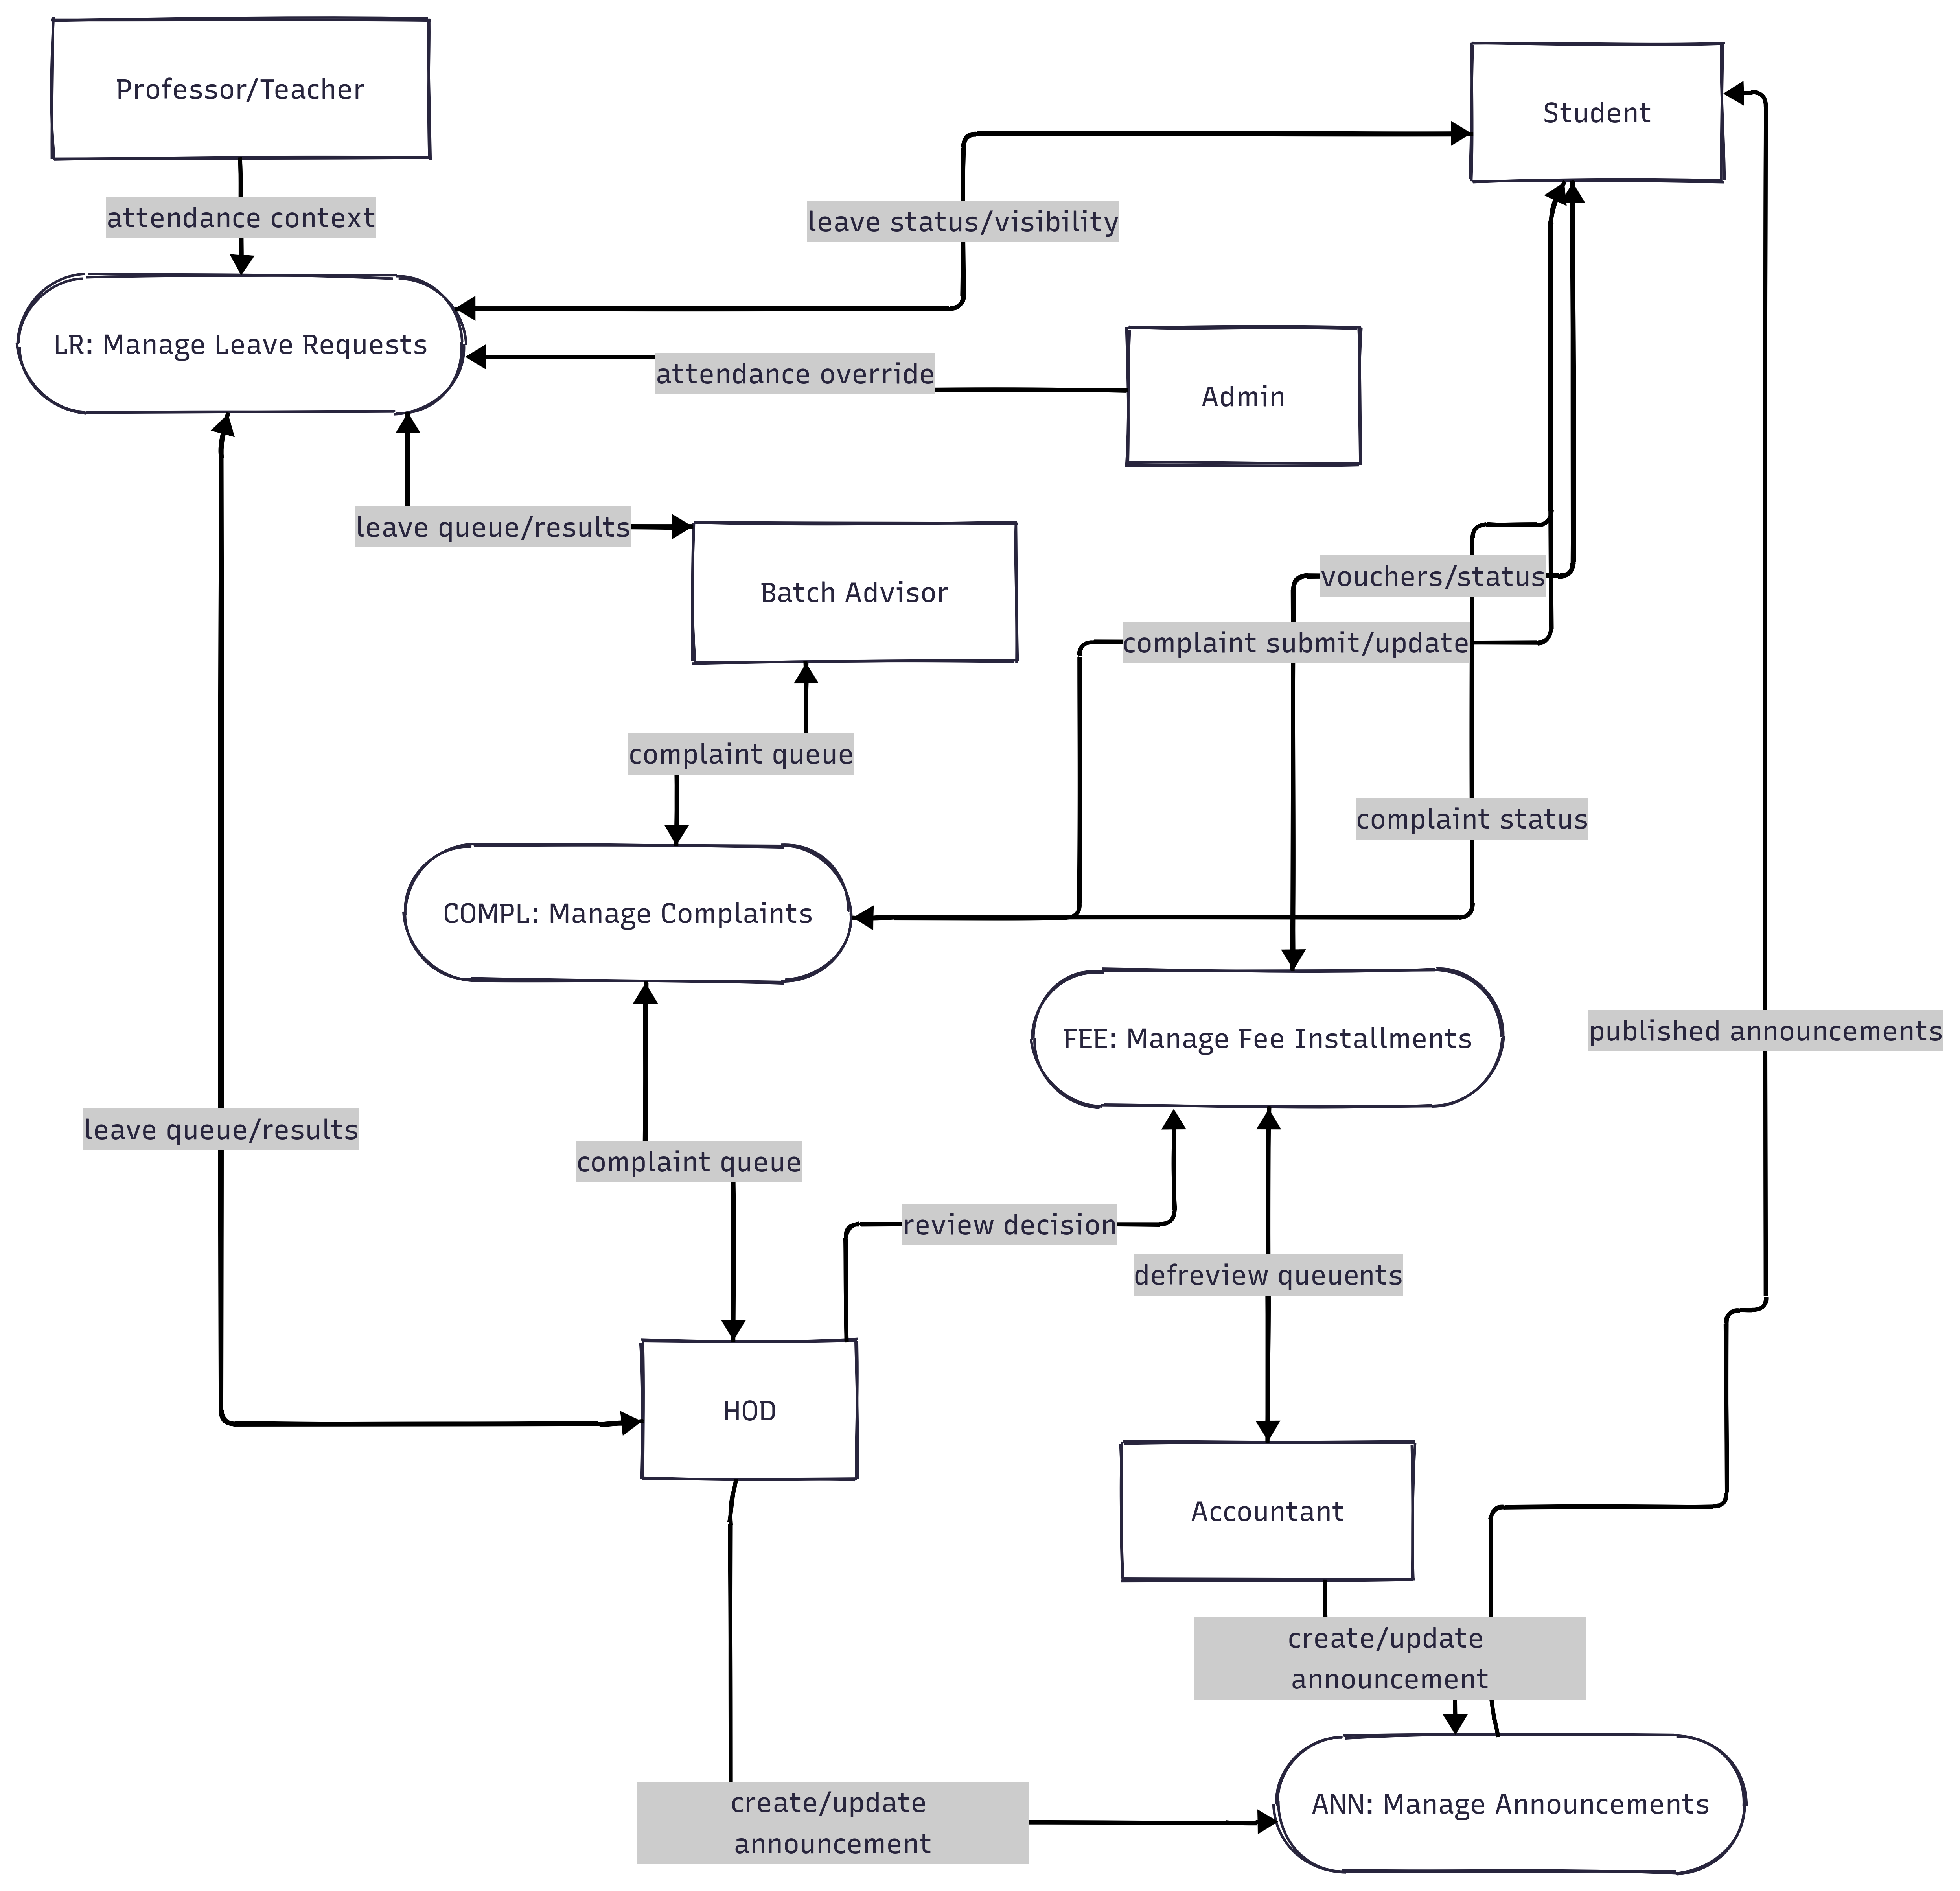
\includegraphics[width=\linewidth]{Figures/diagrams/dfd/dfd-0.png}
  \caption{Data flow - Level 0}
  \label{fig:dfd-0}
\end{figure}


\subsection{Level 1 Data Flow Diagram}

%%%%%%%%%%%%%%%%%%%%%%%%%%%%%%%%%%%%%%%%%%%%%%%%%%%%%%

%%%%%%%%%%%%%%%%%%%%%%%%%%%%%%%%%%%%%%%%%%%%%%%%%%%%%%

\subsubsection{Leave request}

\begin{figure}[H]
  \centering
  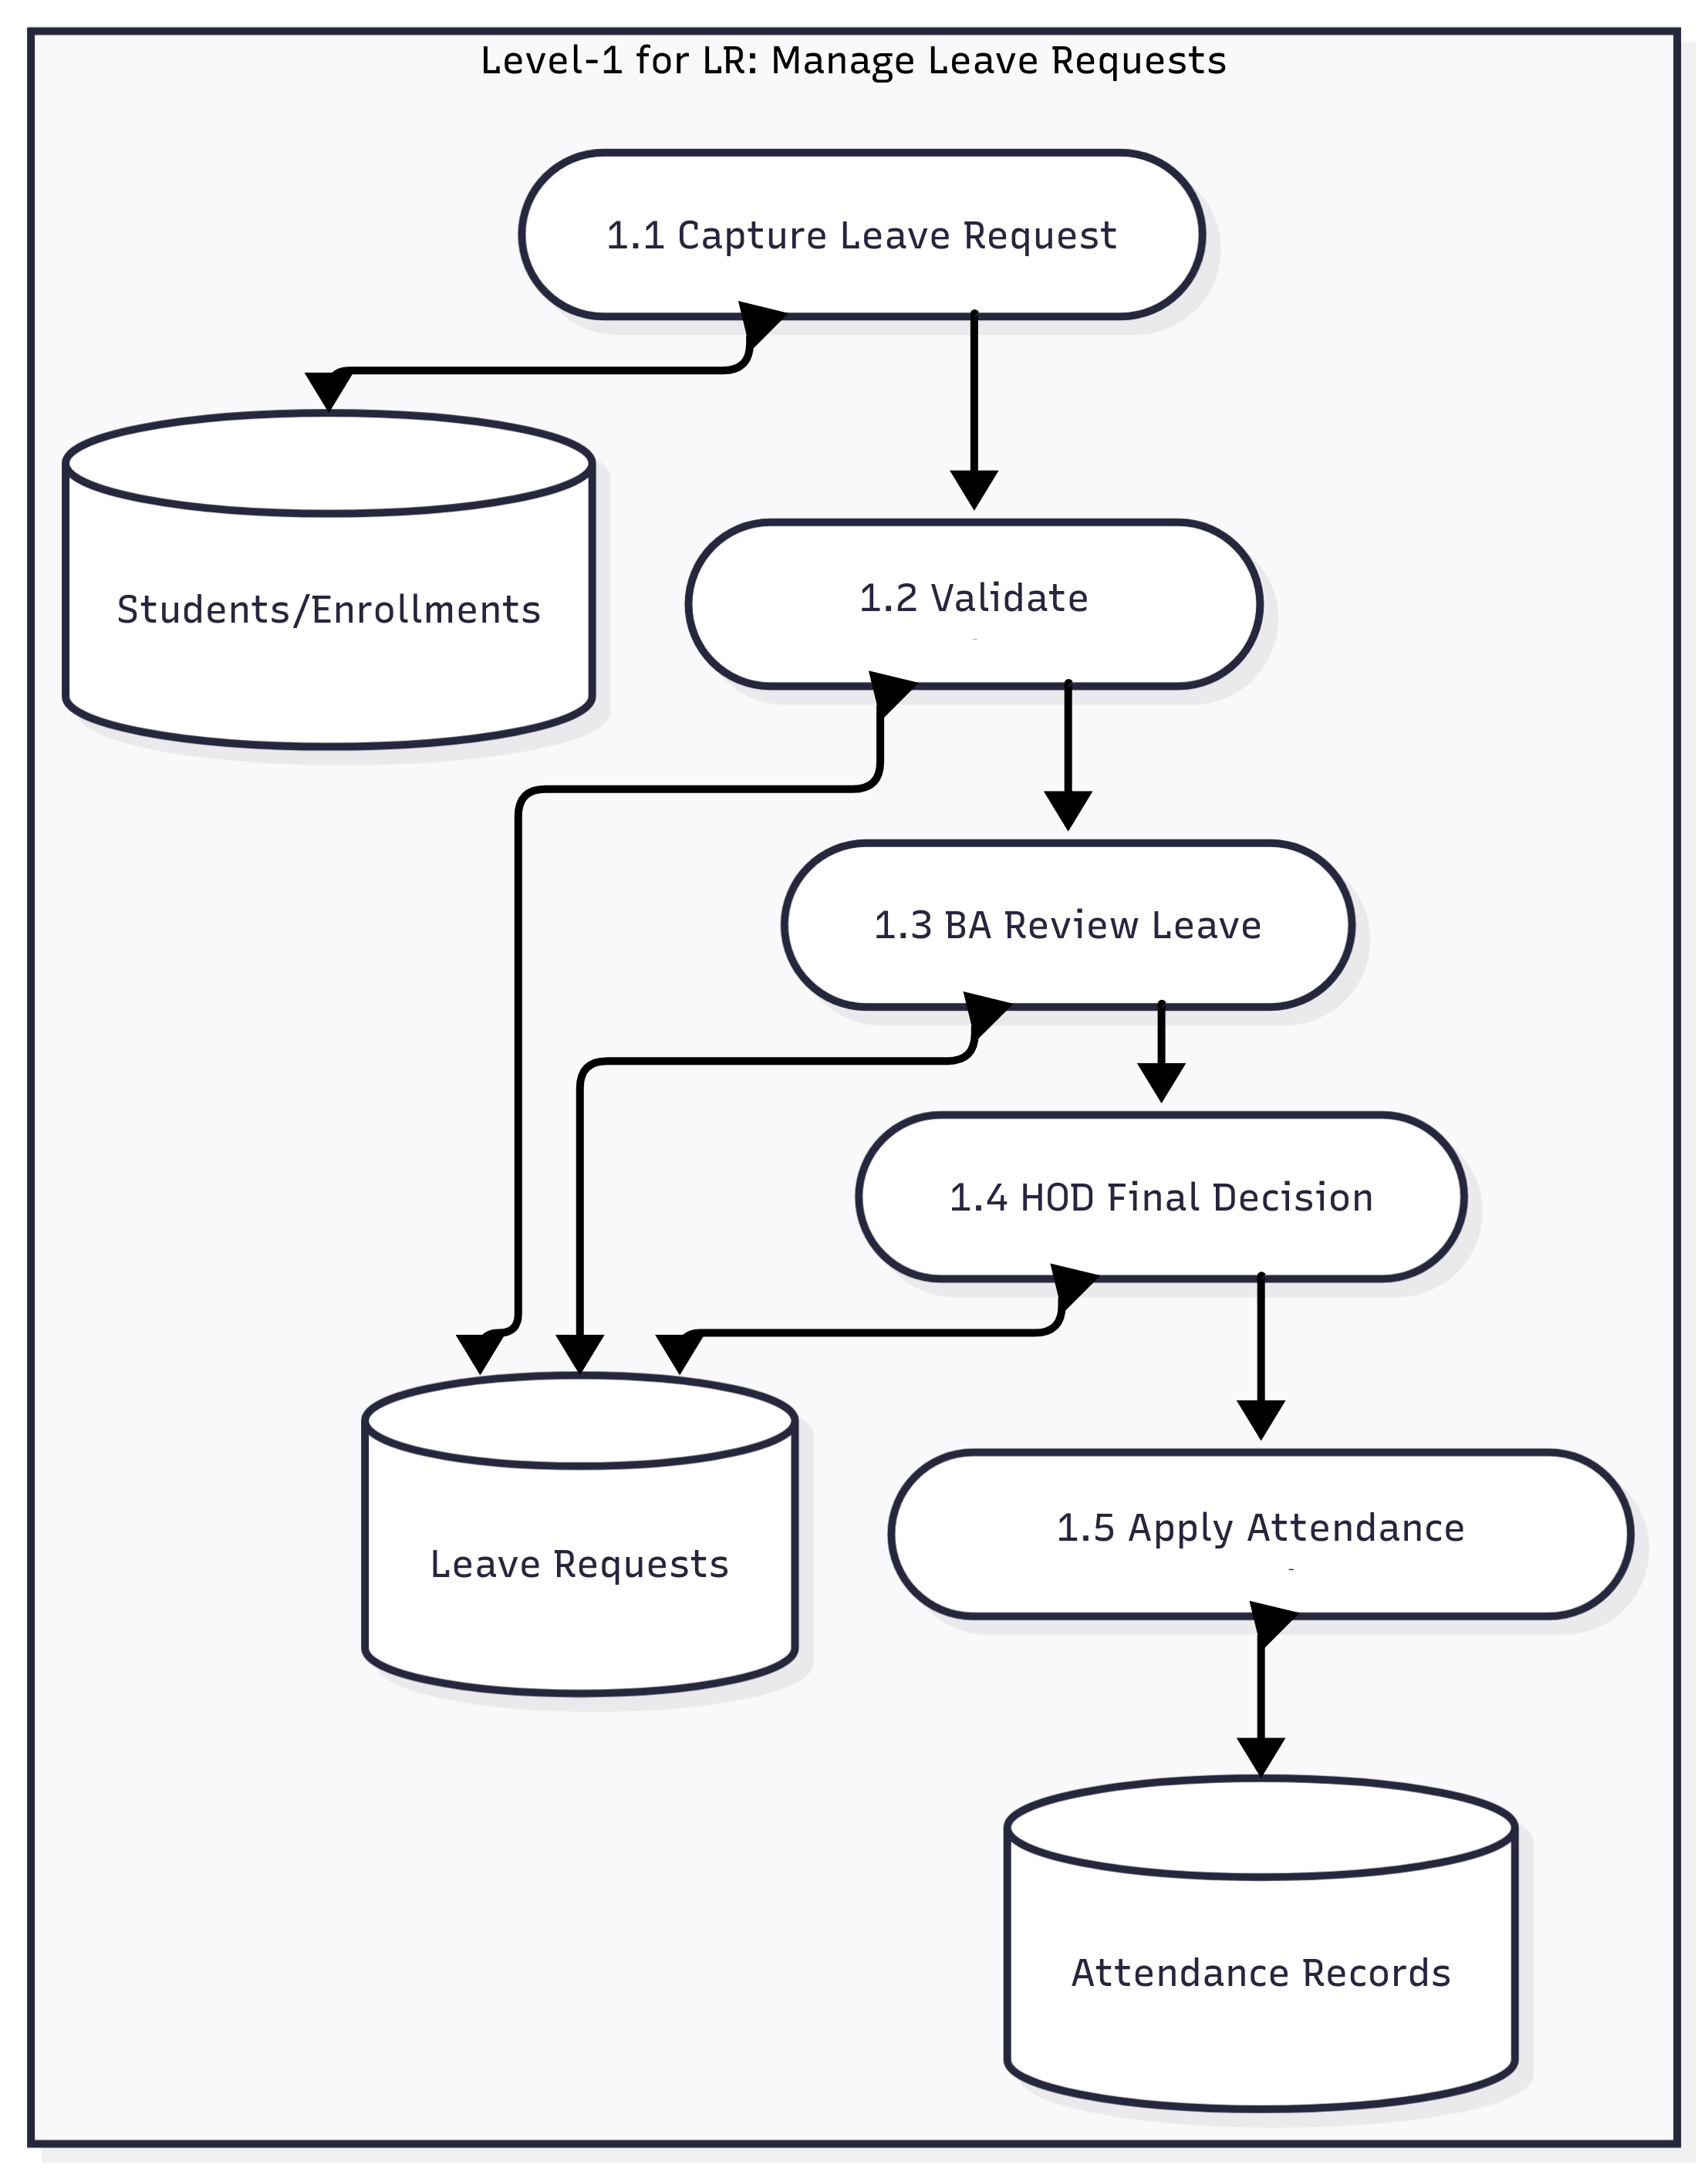
\includegraphics[width=\linewidth]{Figures/diagrams/dfd/dfd-1-lr.png}
  \caption{Data flow lvl-1 - Leave request}
  \label{fig:dfd-1-lr}
\end{figure}


\subsubsection{Complaint}

\begin{figure}[H]
  \centering
  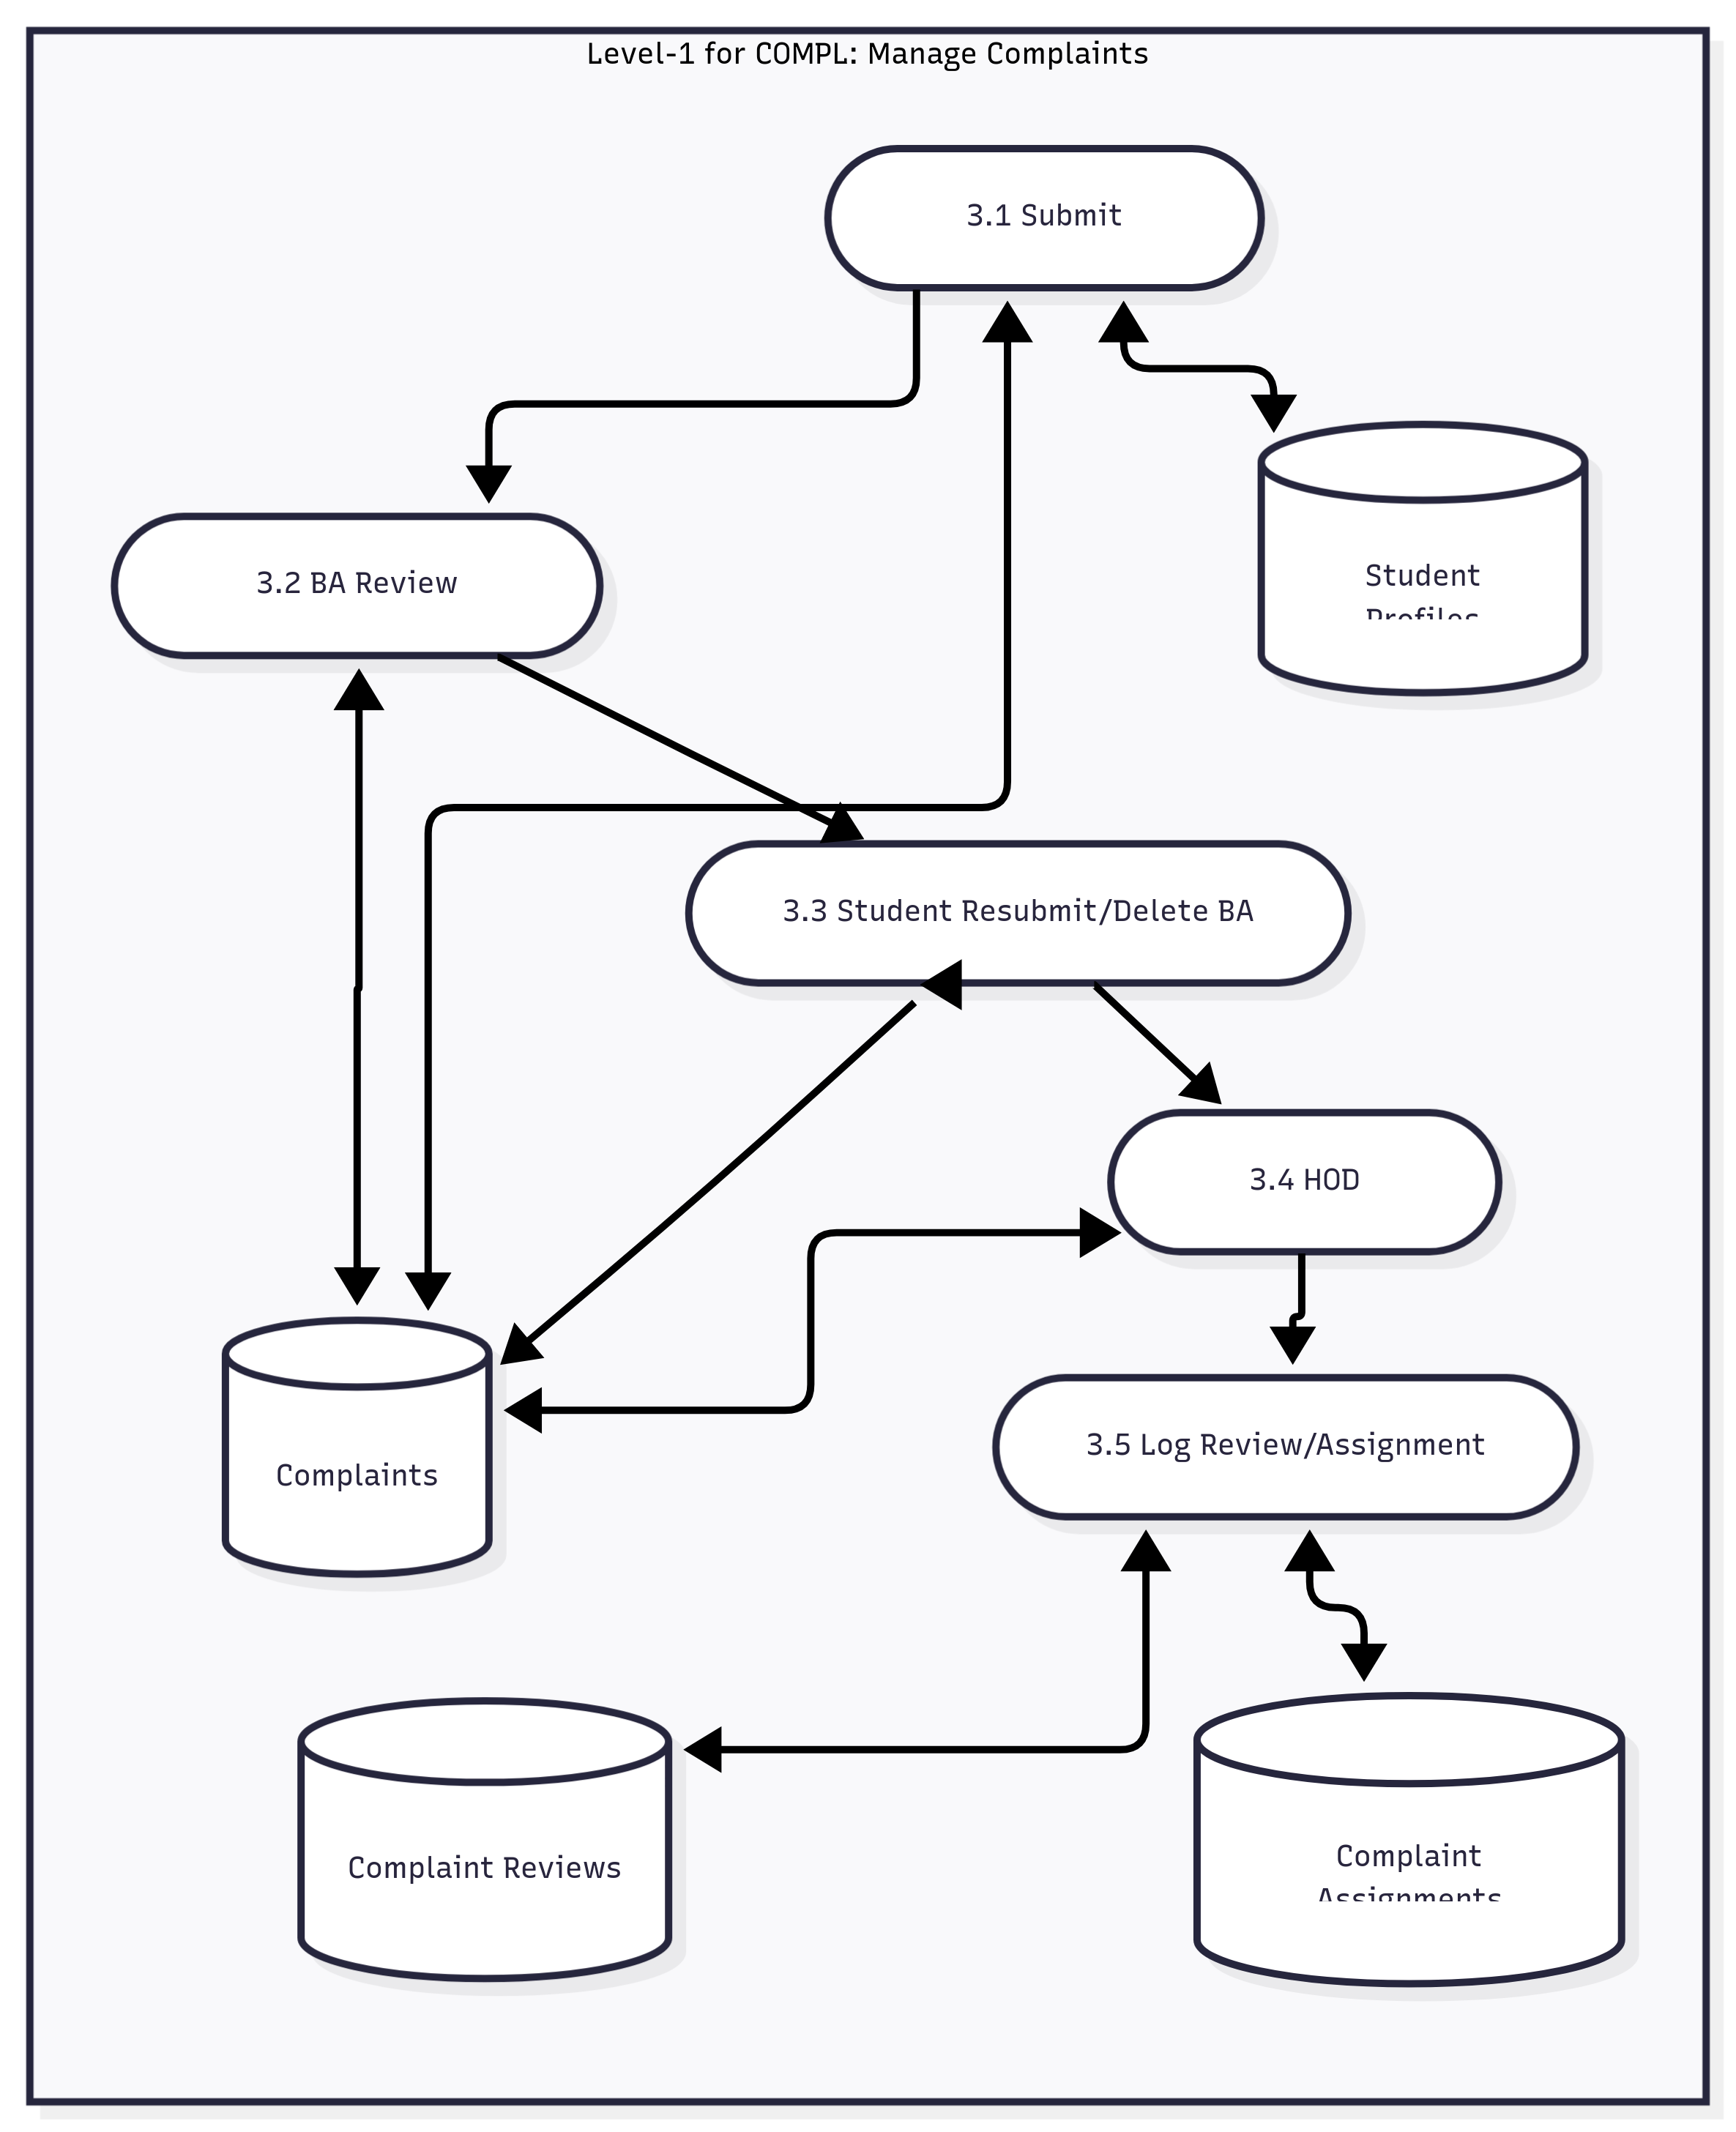
\includegraphics[width=\linewidth]{Figures/diagrams/dfd/dfd-1-compl.png}
  \caption{Data flow lvl-1 - Complaint}
  \label{fig:dfd-1-compl}
\end{figure}


\subsubsection{Fee installment}

\begin{figure}[H]
  \centering
  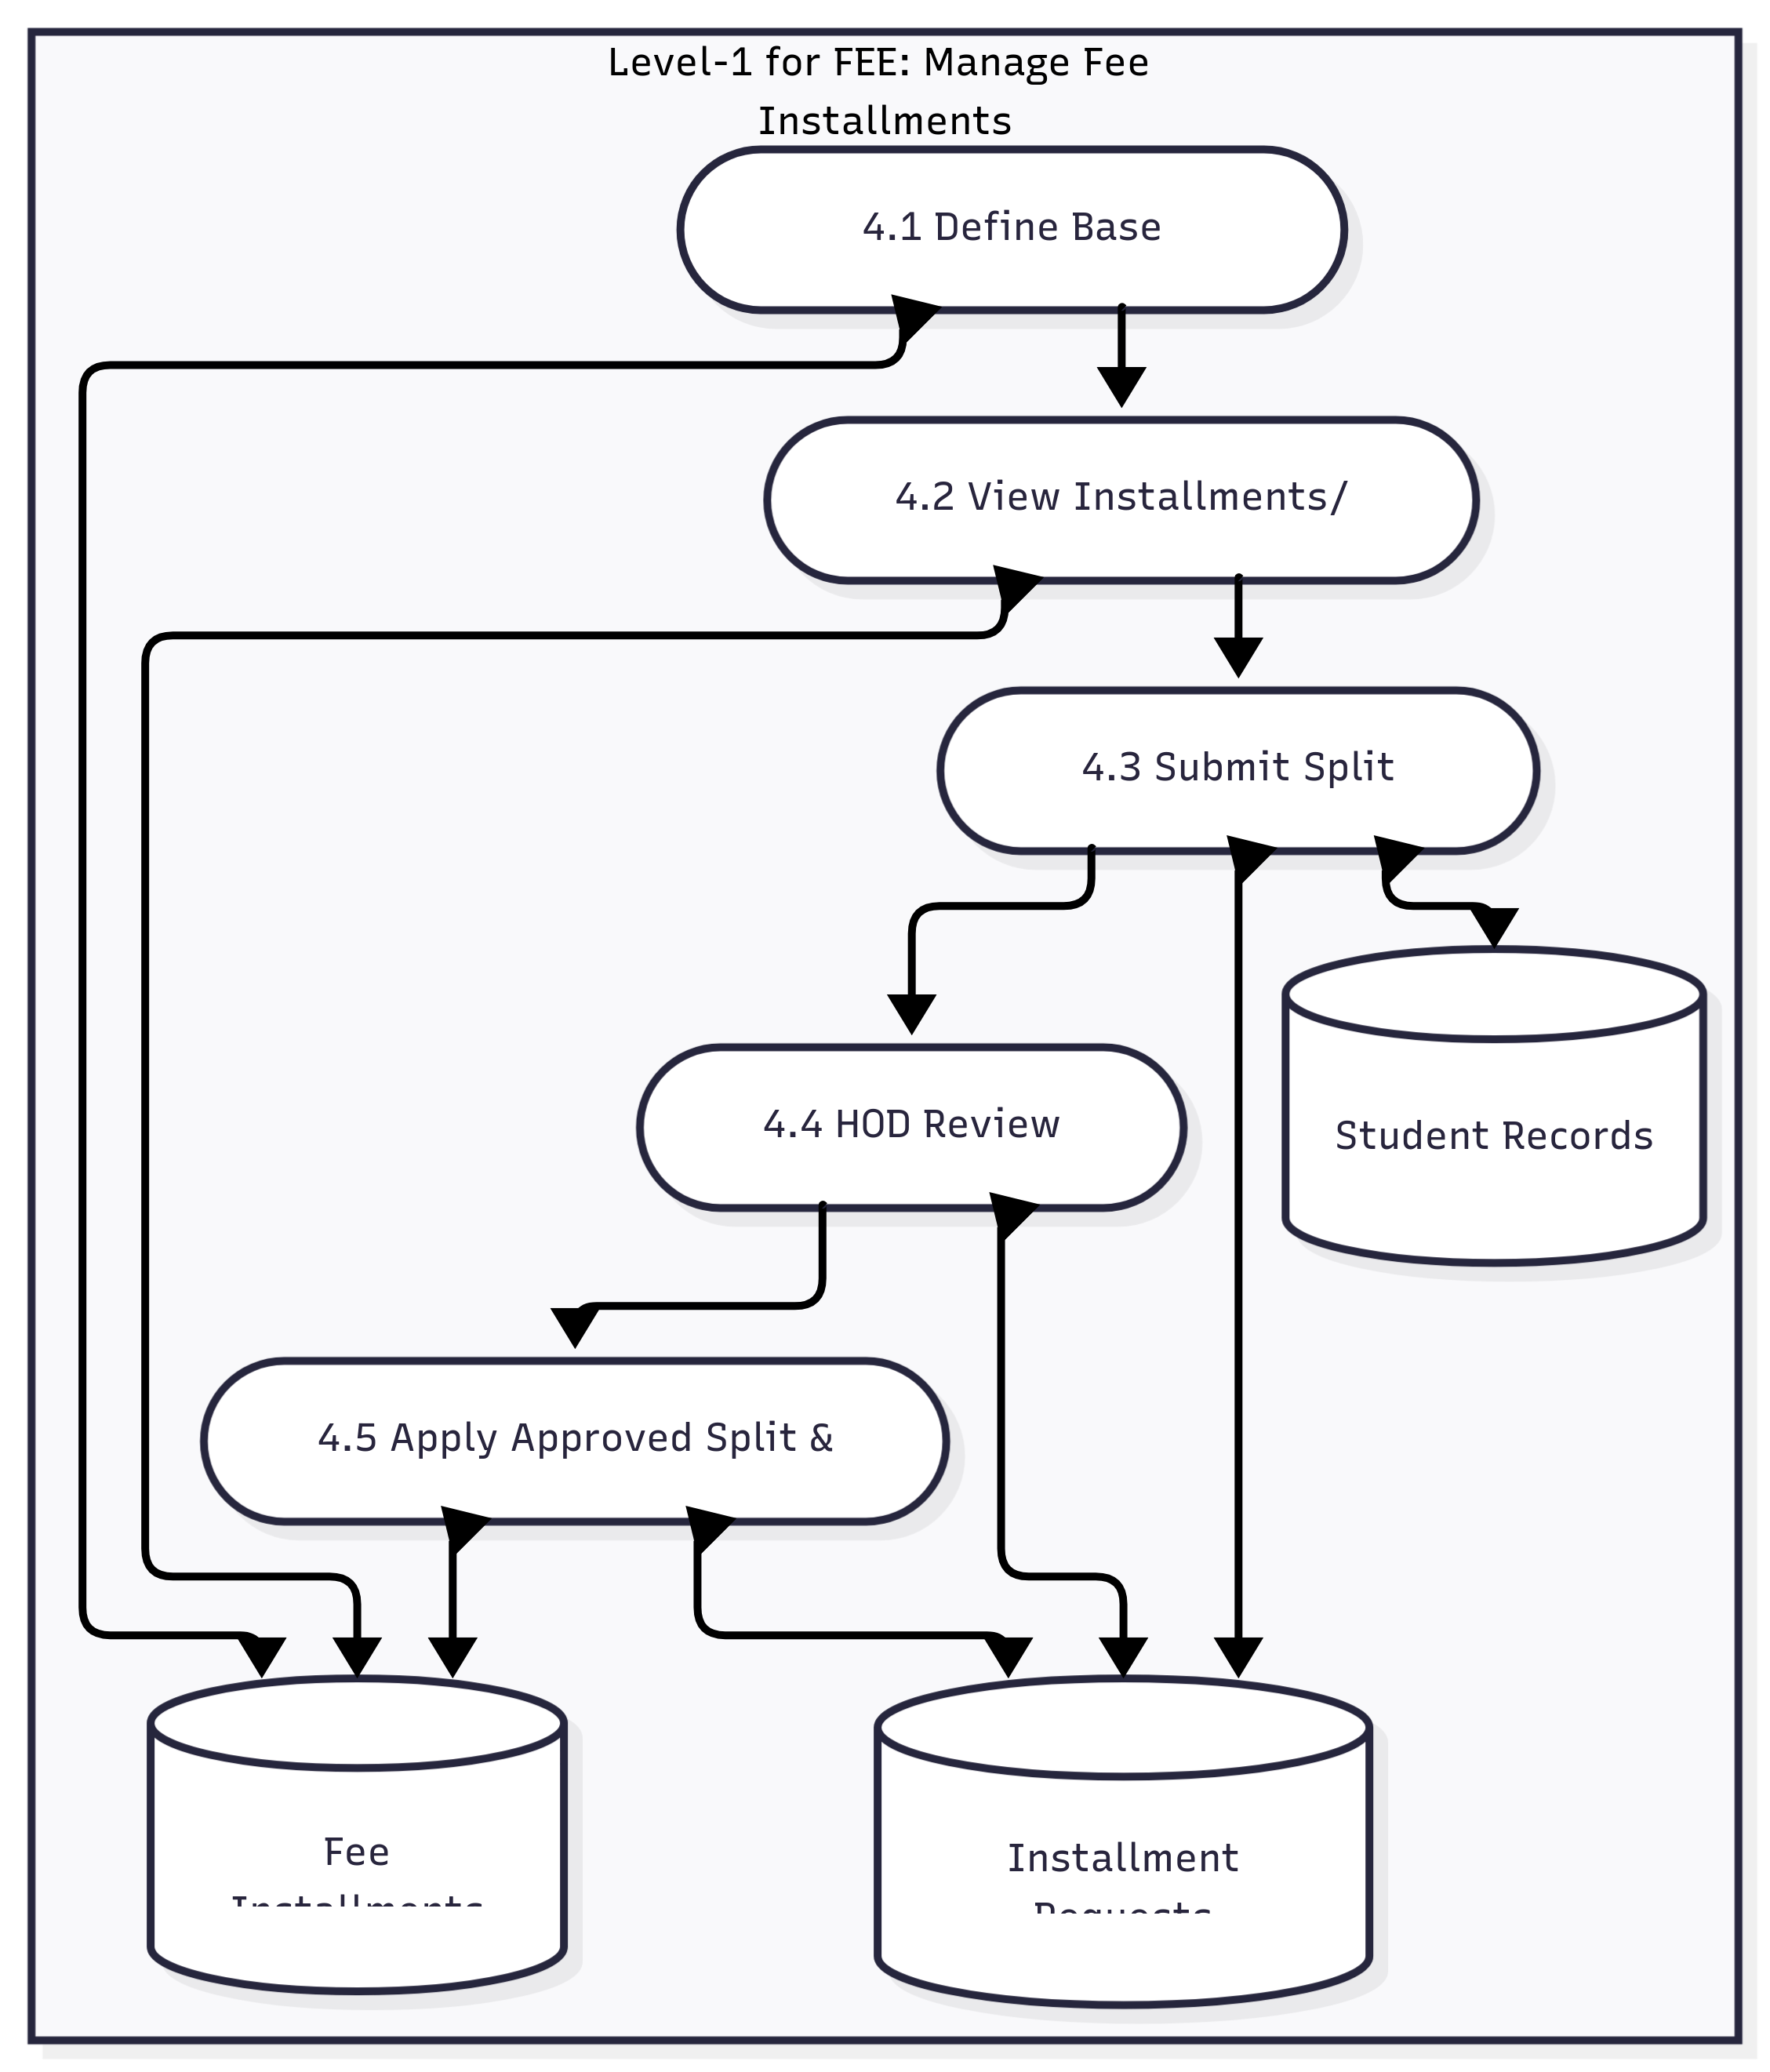
\includegraphics[width=\linewidth]{Figures/diagrams/dfd/dfd-1-fee.png}
  \caption{Data flow lvl-1 - Fee installment}
  \label{fig:dfd-1-fee}
\end{figure}



\subsubsection{Announcements}

\begin{figure}[H]
  \centering
  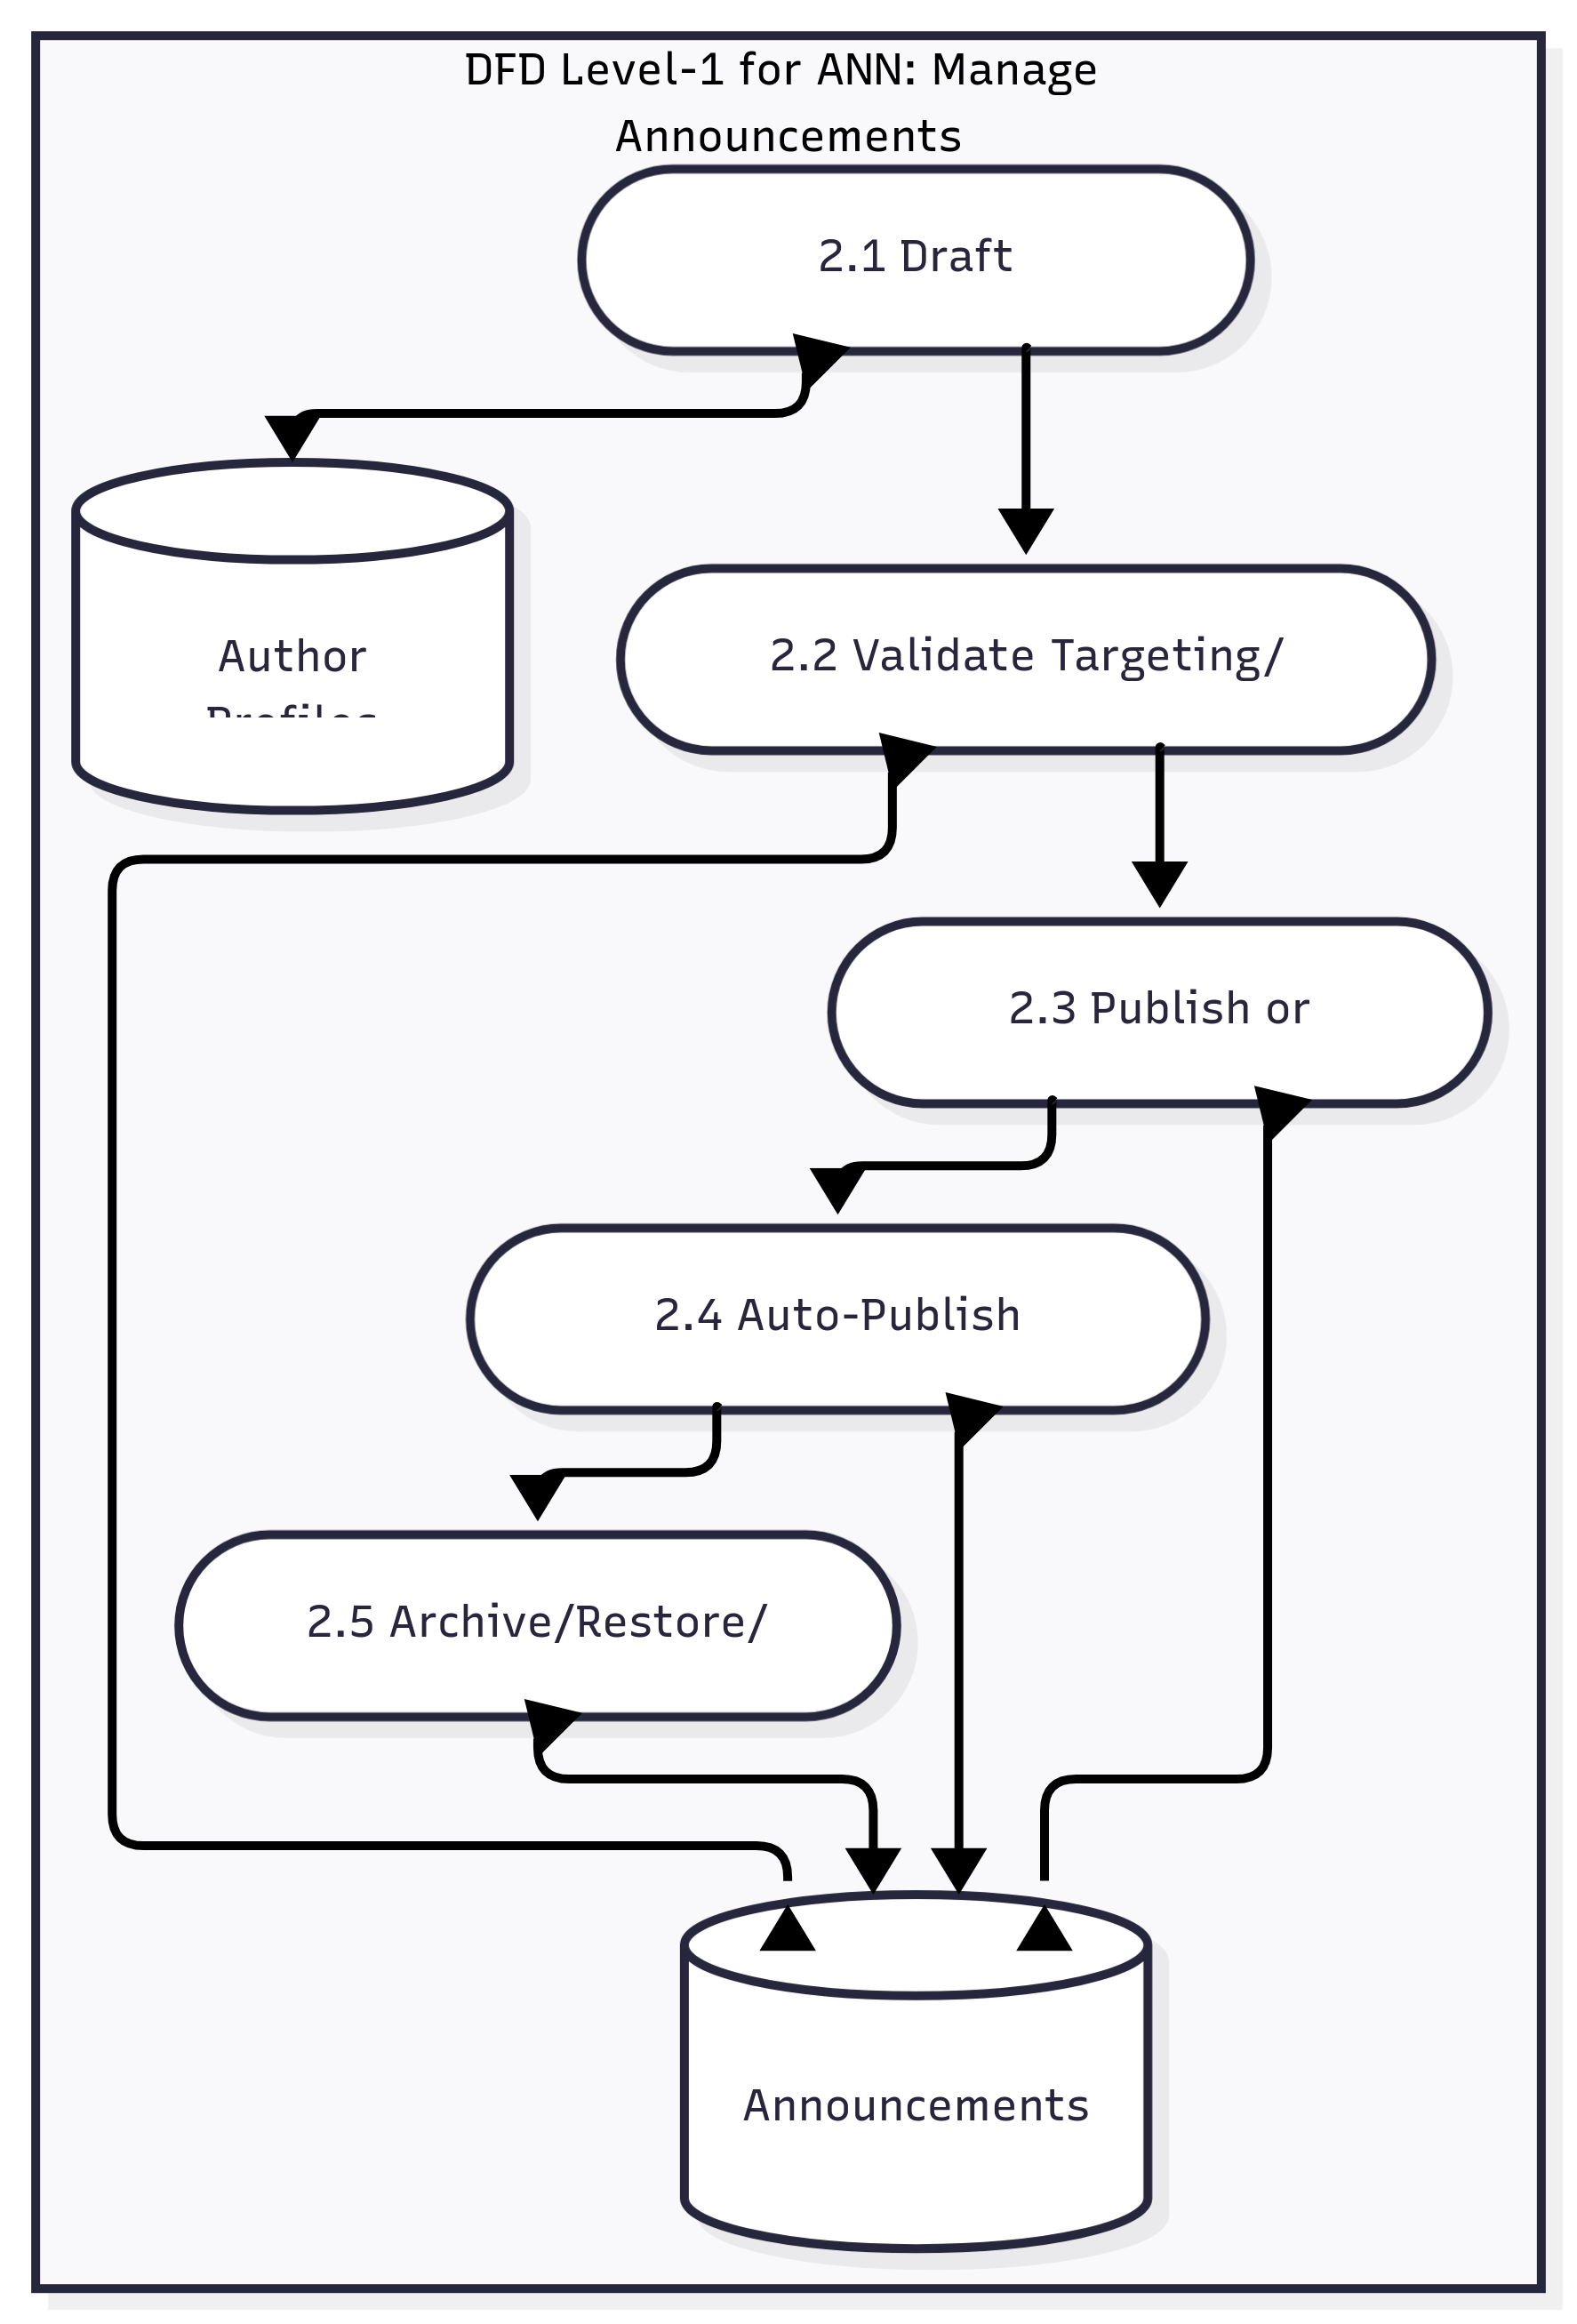
\includegraphics[width=\linewidth]{Figures/diagrams/dfd/dfd-1-ann.png}
  \caption{Data flow lvl-1 - Announcements}
  \label{fig:dfd-1-ann}
\end{figure}


\subsection{Level 2 Data Flow Diagram}

\textbf{Description:}
Level 2 DFD further decomposes one complex module from Level 1.

\subsubsection{Leave requests}

\begin{figure}[H]
  \centering
  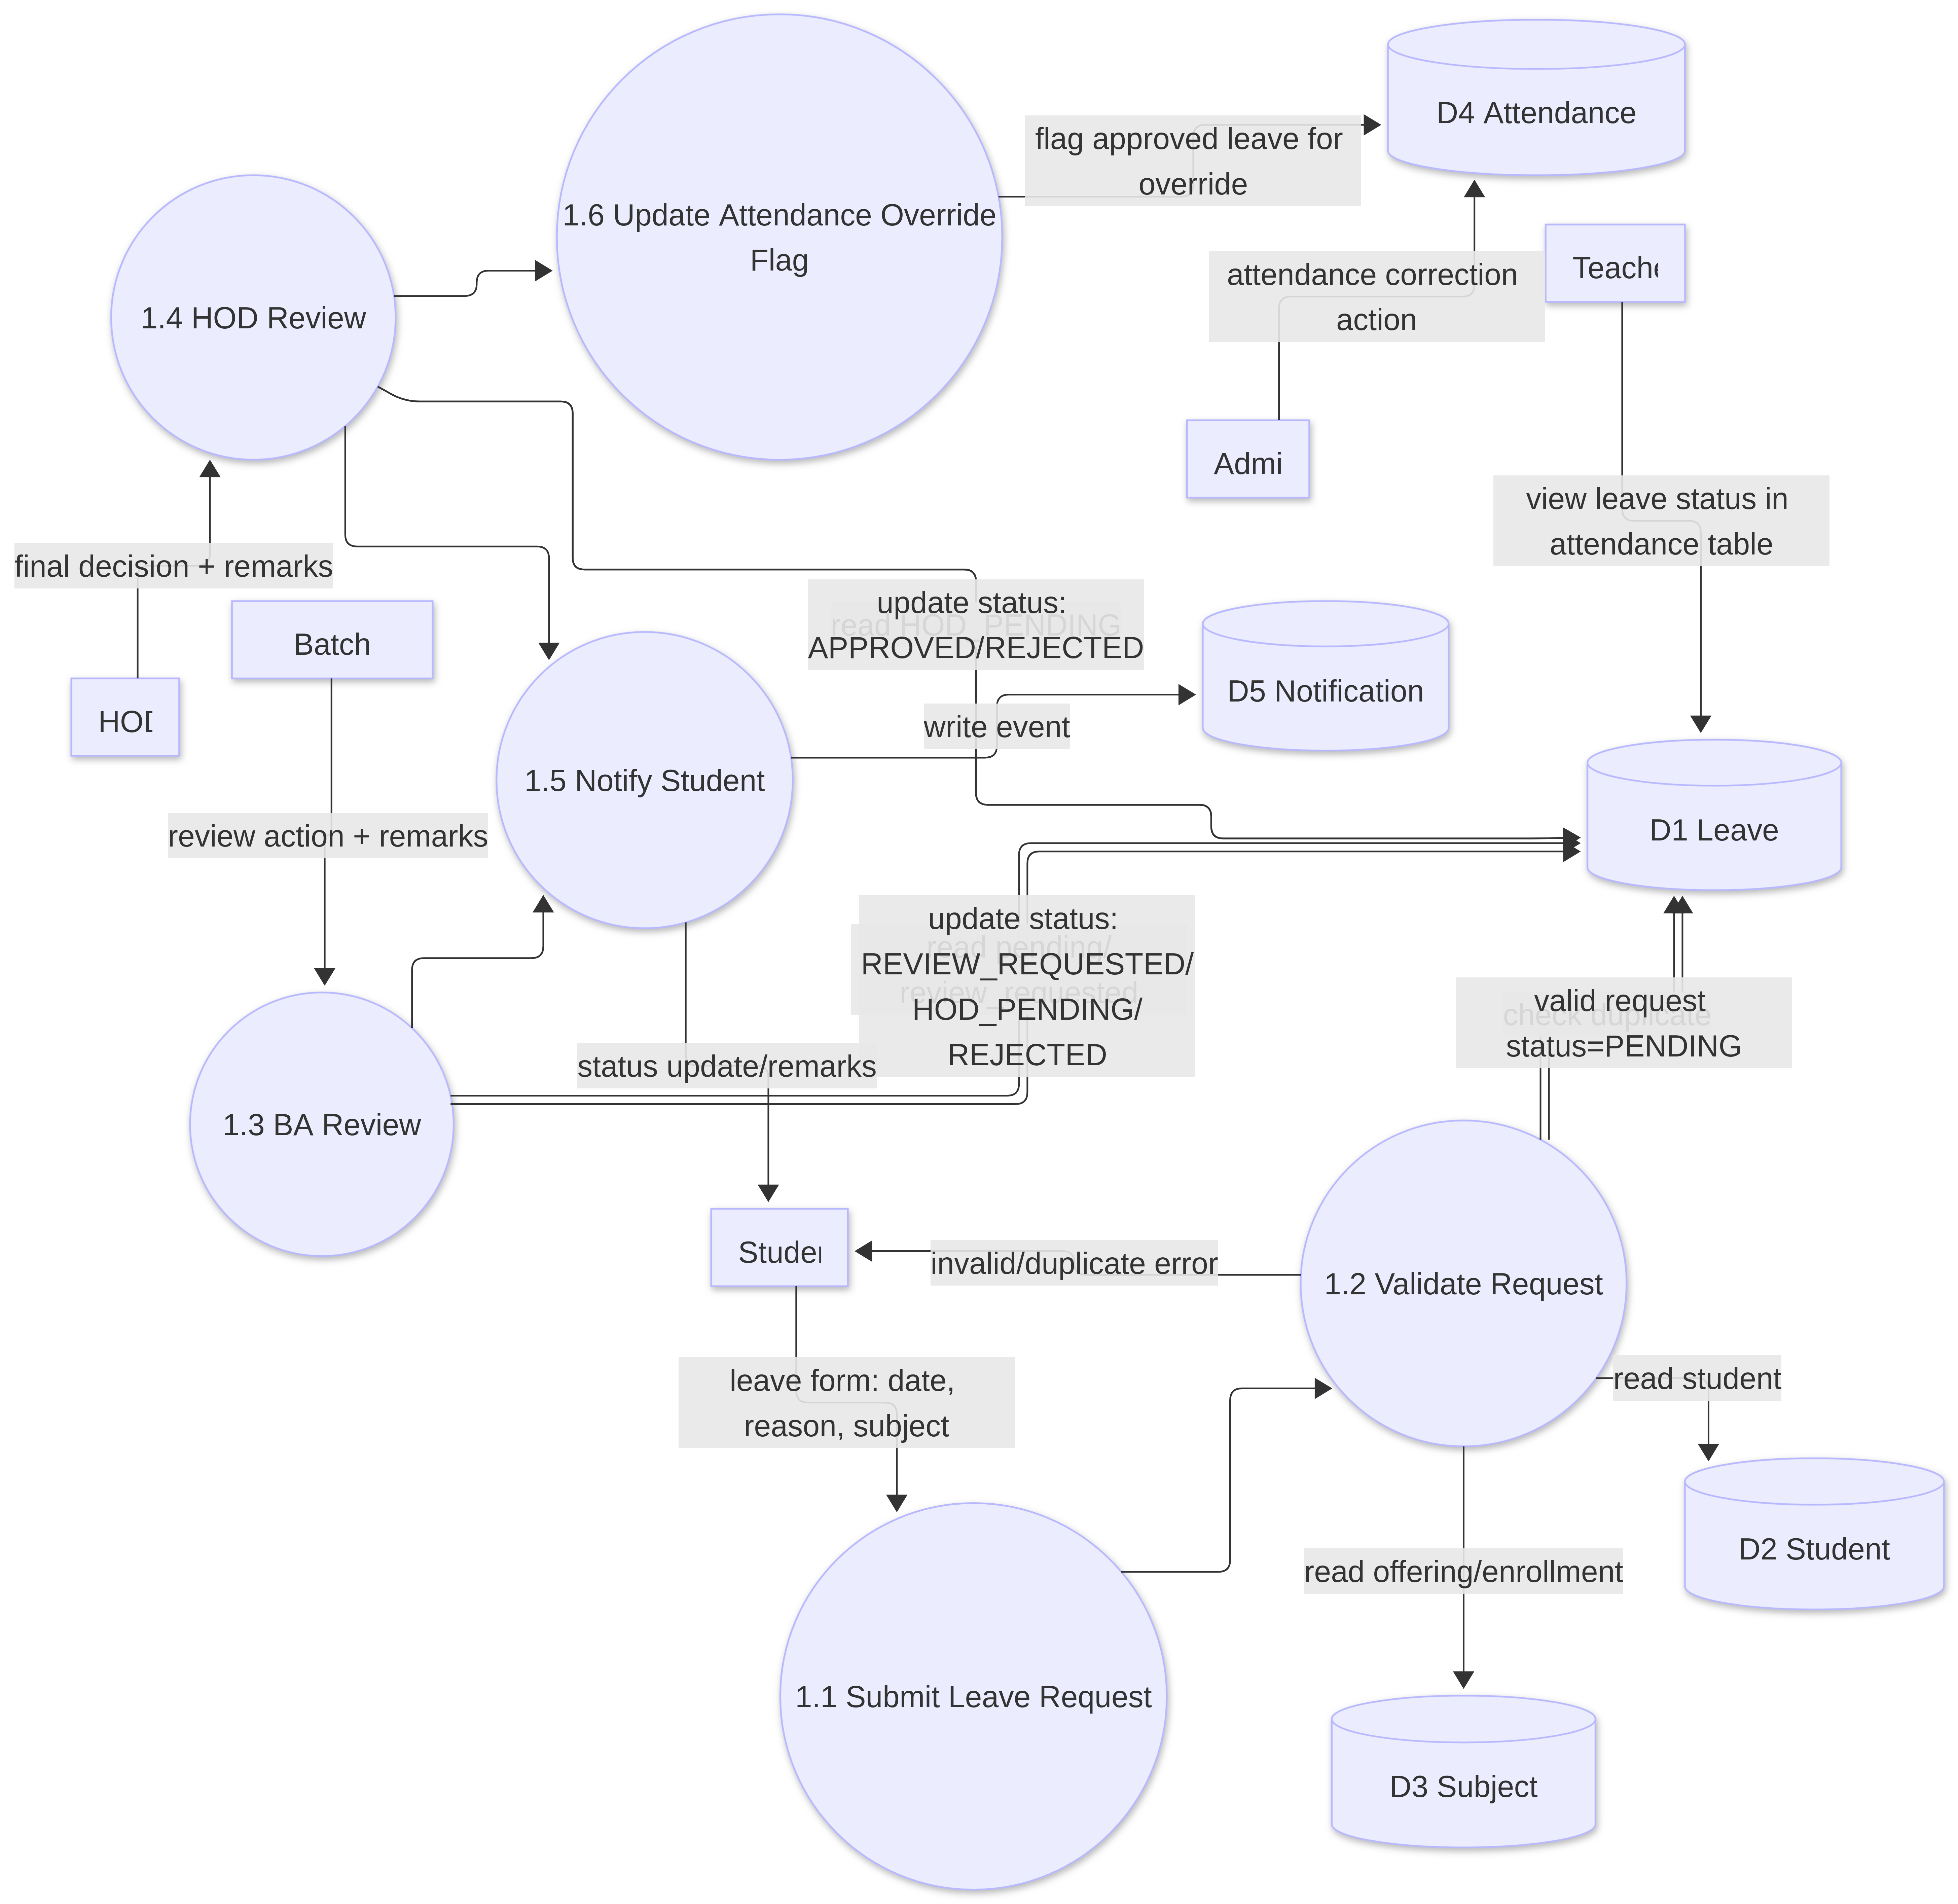
\includegraphics[width=\linewidth]{Figures/diagrams/dfd/dfd-2-lr.png}
  \caption{Data flow lvl-2 - Leave requests}
  \label{fig:dfd-2-lr}
\end{figure}


\subsubsection{Complaint}

\begin{figure}[H]
  \centering
  \includegraphics[width=\linewidth]{Figures/diagrams/dfd/dfd-2-compl.png}
  \caption{Data flow lvl-2 - complaint}
  \label{fig:dfd-2-compl}
\end{figure}


%%%%%%%%%%%%%%%%%%%%%%%%%%%%%%%%%%%%%%%%%%%%%%%%%%%%%%
\section{Data Design}

This section describes how data is structured, stored, and managed.

\textbf{Guidelines:}
\begin{itemize}
    \item \textbf{Database Type:} The system uses \textbf{PostgreSQL} (a relational SQL database) managed via Prisma ORM. This enforces strict relational integrity, handles complex multi-step approval workflows via foreign keys, and safely manages status constraints using DB-level enums.

    \item \textbf{Schema Structure:} The schema is highly normalized into distinct domains (Identity/Roles, Academic, Attendance/Leave, Announcements, and Complaints). Profile data (e.g., student, HOD) is separated from the core \texttt{user} table using 1:1 unique foreign keys. Processes like complaint reviews use immutable, append-only tables to maintain a complete audit trail.

    \item \textbf{Indexing Strategy:} All primary keys utilize UUIDs to prevent sequential ID leakage. The strategy focuses on specific access patterns rather than blanket coverage—leveraging unique constraints to prevent duplicates (e.g., \texttt{studentId, offeringId, date} for leave requests) and utilizing compound indexes for high-frequency queries (e.g., \texttt{status, isPinned, publishedAt} for the announcement feed).

    \item \textbf{Security Mechanisms:} Authentication is securely managed via \texttt{better-auth}. Every mutation enforces strict \texttt{requireSession} and \texttt{requirePermission} checks server-side. Additionally, queries use row-level scoping (restricting visibility to a user's own records or department), foreign keys utilize cascade deletes to prevent orphaned data, and Arcjet rate-limiting mitigates spam/burst traffic on mutations.
    
    \item \textbf{Scalability Considerations:} Time-sensitive operations (like scheduled announcements) are offloaded to \textbf{Inngest} background jobs. Read-heavy feeds are optimized via compound indexing, and append-only audit tables ensure high write volumes don't cause index hot spots.
\end{itemize}

%%%%%%%%%%%%%%%%%%%%%%%%%%%%%%%%%%%%%%%%%%%%%%%%%%%%%%
\subsection{Entity Relationship Diagram (ERD)}

\begin{figure}[H]
  \centering
  
\includegraphics[width=\linewidth]{Figures/diagrams/comsats-erd.png}
  \caption{ERD}
  \label{fig:erd}
\end{figure}

The Entity Relationship Diagram (ERD) represents the logical database structure of the system, illustrating how user roles, academic data, workflows, and audit logs are connected.

\begin{itemize}
    \item \textbf{Entities (Tables):} The database is normalized into distinct domains:
    \begin{itemize}
        \item \textbf{User \& Auth Categories:} \texttt{user}, \texttt{session}, \texttt{account}, \texttt{verification}.
        \item \textbf{User Role Profiles:} \texttt{student}, \texttt{professor}, \texttt{hod}, \texttt{batch\_advisor}, \texttt{accountant}, \texttt{director}.
        \item \textbf{Core Functional \& Academic:} \texttt{subject}, \texttt{subject\_offering}, \texttt{enrollment}, \texttt{registration}, \texttt{teaching\_assignment}.
        \item \textbf{Workflows (Leaves \& Complaints):} \texttt{leave\_request}, \texttt{attendance\_record}, \texttt{student\_attendance}, \texttt{complaint}, \texttt{announcement}.
        \item \textbf{Logs \& Transactions:} \texttt{complaint\_review}, \texttt{complaint\_assignment}.
    \end{itemize}
    \item \textbf{Primary Keys (PK):} Every table utilizes a UUID \texttt{id} as its primary key. This prevents sequential ID enumeration and uniquely identifies each record securely across all domains.
    \item \textbf{Foreign Keys (FK):} Relational integrity is enforced using foreign keys such as \texttt{userId}, \texttt{studentId}, \texttt{offeringId}, and \texttt{complaintId}. These keys ensure valid references between tables (e.g., a \texttt{leave\_request} must reference a valid \texttt{studentId} and \texttt{offeringId}) and facilitate features like cascade deletes where appropriate.
    \item \textbf{Relationship Cardinalities:}
    \begin{itemize}
        \item \textbf{1:1 (One-to-One):} E.g., \texttt{user} to role profiles (a user can have exactly one \texttt{student} or \texttt{professor} profile), \texttt{subject\_offering} to \texttt{teaching\_assignment} (one professor per offering).
        \item \textbf{1:N (One-to-Many):} E.g., \texttt{user} to \texttt{session}, \texttt{student} to \texttt{leave\_request}, \texttt{offering} to \texttt{attendance\_record}, \texttt{complaint} to \texttt{complaint\_review} log entries.
        \item \textbf{M:N (Many-to-Many):} E.g., \texttt{student} and \texttt{subject\_offering} (resolved via the \texttt{enrollment} junction table), where a student can enroll in many offerings and an offering has many students.
    \end{itemize}
\end{itemize}

%%%%%%%%%%%%%%%%%%%%%%%%%%%%%%%%%%%%%%%%%%%%%%%%%%%%%%
\subsection{Database Architecture}

\subsubsection{Client-server architecture}:

The portal follows a standard three-tier client-server model. The browser (client) communicates exclusively with Next.js server actions — no direct DB access from the client. Prisma ORM sits between the application layer and PostgreSQL, handling query building and type safety. Better-auth manages session validation on every request before any business logic or DB query executes.


%%%%%%%%%%%%%%%%%%%%%%%%%%%%%%%%%%%%%%%%%%%%%%%%%%%%%%
\section{Database Schema Diagram}

\begin{figure}[H]
  \centering
  
\includegraphics[width=\linewidth]{Figures/diagrams/comsats-erd.png}
  \caption{Database schema diagram}
  \label{fig:db-schema}
\end{figure}


The Database Schema Diagram visually represents the physical database implementation, mapping the core system modules—including identity management, academic structures, targeted operational workflows, and immutable audit logs—along with their relational bindings and cardinality constraints. The schema ensures \textbf{data integrity} using strict PostgreSQL relational constraints, unique foreign keys with cascade deletes, and DB-level enums managed by Prisma ORM. \textbf{Efficient querying} is achieved through targeted compound indexes optimized for frequent read operations, such as announcement feeds. For \textbf{scalability}, UUID primary keys prevent database index hotspots, while immutable append-only audit tables smoothly handle growing data volumes. Lastly, \textbf{security} is maintained by Better-Auth's session management—storing only hashed credentials—alongside Arcjet rate-limiting on database mutations.


%%%%%%%%%%%%%%%%%%%%%%%%%%%%%%%%%%%%%%%%%%%%%%%%%%%%%%
\subsection{Data Dictionary}

Data Dictionary defines structure of all data elements.

\begin{table}[H]
\centering
\caption{Data Dictionary – User and Auth Fields}
\begin{tabularx}{\textwidth}{|p{2.5cm}|p{2cm}|p{1.2cm}|X|p{2.5cm}|}
\hline
\textbf{Field Name} & \textbf{Data Type} & \textbf{Size} & \textbf{Description} & \textbf{Constraints} \\
\hline
id & UUID & 36 & Unique identifier for records & PK \\
\hline
email & String & 255 & User email address & Required, Unique \\
\hline
name & String & 255 & Full name of the user & Required \\
\hline
role & Enum & - & Access role designation & Required \\
\hline
password & String & 255 & Hashed user password & Required \\
\hline
token & String & 255 & Active session token & Required, Unique \\
\hline
expiresAt & DateTime & - & Expiry for sessions/tokens & Required \\
\hline
banned & Boolean & - & Account suspension flag & Default False \\
\hline
\end{tabularx}
\end{table}

%%%%%%%%%%%%%%%%%%%%%%%%%%%%%%%%%%%%%%%%%%%%%%%%%%%%%%
\begin{table}[H]
\centering
\caption{Data Dictionary – Role Profile Fields}
\begin{tabularx}{\textwidth}{|p{2.5cm}|p{2cm}|p{1.2cm}|X|p{3cm}|}
\hline
\textbf{Field Name} & \textbf{Data Type} & \textbf{Size} & \textbf{Description} & \textbf{Constraints} \\
\hline
userId & UUID & 36 & Parent user mapping & FK, Required, Unique \\
\hline
registrationNo & String & 50 & Unique student identifier & Required, Unique \\
\hline
employeeNo & String & 50 & Unique employee identifier & Required, Unique \\
\hline
department & String & 100 & Base department for user & Required \\
\hline
program & String & 100 & Degree program & Required \\
\hline
appointedAt & DateTime & - & Date BA was appointed & Required \\
\hline
\end{tabularx}
\end{table}

%%%%%%%%%%%%%%%%%%%%%%%%%%%%%%%%%%%%%%%%%%%%%%%%%%%%%%
\begin{table}[H]
\centering
\caption{Data Dictionary – Academic Fields}
\begin{tabularx}{\textwidth}{|p{2.5cm}|p{2cm}|p{1.2cm}|X|p{3cm}|}
\hline
\textbf{Field Name} & \textbf{Data Type} & \textbf{Size} & \textbf{Description} & \textbf{Constraints} \\
\hline
subjectId & UUID & 36 & Reference to global subject & FK, Required \\
\hline
code & String & 20 & Global subject code & Required, Unique \\
\hline
creditHours & Int & 2 & Credit hours for subject & Required, > 0 \\
\hline
semester & Int & 2 & Current offering semester & Required \\
\hline
year & Int & 4 & Academic calendar year & Required \\
\hline
section & String & 10 & Class section identifier & Optional \\
\hline
totalLectures & Int & 3 & Count of semester lectures & Required, Default 0 \\
\hline
\end{tabularx}
\end{table}

%%%%%%%%%%%%%%%%%%%%%%%%%%%%%%%%%%%%%%%%%%%%%%%%%%%%%%
\begin{table}[H]
\centering
\caption{Data Dictionary – Operational Fields}
\begin{tabularx}{\textwidth}{|p{2.5cm}|p{2cm}|p{1.2cm}|X|p{3cm}|}
\hline
\textbf{Field Name} & \textbf{Data Type} & \textbf{Size} & \textbf{Description} & \textbf{Constraints} \\
\hline
status & Enum & - & Current workflow progress state & Required \\
\hline
date & Date & - & Target date for leave/attendance & Required \\
\hline
title & String & 255 & Header for announcements & Required \\
\hline
category & String & 100 & Classification metric for reports & Required \\
\hline
targetDepartment& String & 100 & Recipient department routing & Required \\
\hline
scheduledFor & DateTime & - & Future publish timestamp & Optional \\
\hline
isPinned & Boolean & - & Dashboard priority rendering & Default False \\
\hline
\end{tabularx}
\end{table}

%%%%%%%%%%%%%%%%%%%%%%%%%%%%%%%%%%%%%%%%%%%%%%%%%%%%%%
\begin{table}[H]
\centering
\caption{Data Dictionary – Audit and Log Fields}
\begin{tabularx}{\textwidth}{|p{2.5cm}|p{2cm}|p{1.2cm}|X|p{3cm}|}
\hline
\textbf{Field Name} & \textbf{Data Type} & \textbf{Size} & \textbf{Description} & \textbf{Constraints} \\
\hline
complaintId & UUID & 36 & Parent ticket reference & FK, Required \\
\hline
action & String & 50 & Audit action performed & Required \\
\hline
actorRole & Enum & - & Role of the acting user & Required \\
\hline
fromStatus & Enum & - & Previous workflow state & Required \\
\hline
toStatus & Enum & - & Resulting workflow state & Required \\
\hline
remarks & Text & - & Reviewer qualitative notes & Optional \\
\hline
fromDepartment & String & 100 & Original department assignment& Required \\
\hline
\end{tabularx}
\end{table}


%%%%%%%%%%%%%%%%%%%%%%%%%%%%%%%%%%%%%%%%%%%%%%%%%%%%%%
\subsection{Core Data Collection}
%%%%%%%%%%%%%%%%%%%%%%%%%%%%%%%%%%%%%%%%%%%%%%%%%%%%%%

This subsection describes domain-specific core data tables or collections. These structures store primary operational data processed by the system.
\begin{itemize}
    \item User Table - Stores authentication and role-based identity data.
    \item Student Table - Stores student profile and academic program details.
    \item Professor Table - Stores faculty profile and departmental data.
    \item Subject Offering Table - Stores semester-wise subject allocation details.
    \item Registration Table - Stores student registration requests and status.
    \item Enrollment Table - Stores subject enrollment records for students.
    \item Attendance Record Table - Stores lecture-wise attendance sessions.
    \item Student Attendance Table - Stores attendance status for each student in a session.
    \item Leave Request Table - Stores student leave applications and approval status.
    \item Complaint Table - Stores student complaint records and department routing.
    \item Announcement Table - Stores notices and communication posted by staff.
    \item Review Tables - Stores workflow logs for leave requests, complaints, and registrations.
\end{itemize}

%%%%%%%%%%%%%%%%%%%%%%%%%%%%%%%%%%%%%%%%%%%%%%%%%%%%%%
\subsection{Relationships Between Tables}
%%%%%%%%%%%%%%%%%%%%%%%%%%%%%%%%%%%%%%%%%%%%%%%%%%%%%%

Database relationships define how data entities are connected within the system.

\begin{itemize}
    \item \textbf{One-to-One (1:1):} Each user may have one role-specific profile record such as Student, Professor, HOD, Clerk, Accountant, Director, or Batch Advisor.
    \item \textbf{One-to-Many (1:N):} One user may create multiple announcements, one student may submit multiple leave requests or complaints, and one subject offering may have multiple attendance records.
    \item \textbf{Many-to-Many (M:N):} Students may enroll in multiple subject offerings, and each subject offering may contain many students. This relationship is resolved using the Enrollment table.
\end{itemize}

An Entity-Relationship (ER) Diagram should be included to visually represent these relationships.

%%%%%%%%%%%%%%%%%%%%%%%%%%%%%%%%%%%%%%%%%%%%%%%%%%%%%%
\subsection{Security and Data Integrity}
%%%%%%%%%%%%%%%%%%%%%%%%%%%%%%%%%%%%%%%%%%%%%%%%%%%%%%

To ensure confidentiality and integrity of stored data, the following measures are implemented:

\begin{itemize}
    \item Passwords are stored using secure hashing algorithms.
    \item Role-Based Access Control (RBAC) is used to restrict access based on user roles.
    \item Database constraints such as primary keys, foreign keys, unique fields, and not-null rules are enforced.
    \item Input validation is applied to prevent invalid or unsafe data entry.
\end{itemize}


%%%%%%%%%%%%%%%%%%%%%%%%%%%%%%%%%%%%%%%%%%%%%%%%%%%%%%
\subsection{Scalability Considerations}
%%%%%%%%%%%%%%%%%%%%%%%%%%%%%%%%%%%%%%%%%%%%%%%%%%%%%%

The database design incorporates scalability mechanisms to support future growth and increasing user load.

\begin{itemize}
    \item Indexing is applied on frequently queried fields such as user roles, department, status, and foreign keys to improve query performance.
    \item Caching may be used for frequently accessed records such as announcements, semester data, and subject offerings.
    \item Database queries are structured to minimize unnecessary joins and support efficient retrieval.
    \item Data growth can be managed through partitioning of large transactional tables such as attendance and review logs if needed in the future.
    \item The system is designed to support scaling of the application layer and database layer as demand increases.
\end{itemize}


%%%%%%%%%%%%%%%%%%%%%%%%%%%%%%%%%%%%%%%%%%%%%%%%%%%%%%
\section{Chapter Summary}
%%%%%%%%%%%%%%%%%%%%%%%%%%%%%%%%%%%%%%%%%%%%%%%%%%%%%%

This chapter presented the comprehensive software design of the proposed system.
It translated the functional and non-functional requirements identified earlier
into structured architectural, behavioral, and data models.

The design methodology and selected software process model were justified to
ensure systematic development and maintainability. A high-level system overview
was provided through the context diagram and architectural representation,
clearly illustrating component interactions and subsystem boundaries.

Detailed UML models including activity diagrams, class diagrams, sequence diagrams,
and state transition diagrams were developed to describe system behavior and structure.
Additionally, data flow diagrams were constructed to represent internal data movement
across different system layers.

The chapter further elaborated the database design through Entity Relationship Diagrams,
database schema diagrams, and data dictionaries to ensure data integrity, scalability,
and security. Relationships between entities and normalization considerations were
also addressed.

Overall, this chapter establishes a clear technical blueprint that guides the
implementation phase discussed in the next chapter.
